\date{}
\title{}
\date{}
\begin{document}
\begin{frame}
    \titlepage
\end{frame}

\makeatletter
\newenvironment<>{btHighlight}[1][]
{\begin{onlyenv}#2\begingroup\tikzset{bt@Highlight@par/.style={#1}}\begin{lrbox}{\@tempboxa}}
{\end{lrbox}\bt@HL@box[bt@Highlight@par]{\@tempboxa}\endgroup\end{onlyenv}}

\newcommand<>\btHL[1][]{%
  \only#2{\begin{btHighlight}[#1]\bgroup\aftergroup\bt@HL@endenv}%
}
\def\bt@HL@endenv{%
  \end{btHighlight}%   
  \egroup %
}
\tikzset{
    btHLbox/.style={
        fill=red!30,outer sep=0pt,inner xsep=1pt, inner ysep=0pt, rounded corners=3pt
    },
}
\newcommand{\bt@HL@box}[2][]{%
  \tikz[#1]{%
    \pgfpathrectangle{\pgfpoint{1pt}{0pt}}{\pgfpoint{\wd #2}{\ht #2}}%
    \pgfusepath{use as bounding box}%
    \node[text width={},draw=none,anchor=base west, btHLbox, minimum height=\ht\strutbox+1pt,#1]{\raisebox{1pt}{\strut}\strut\usebox{#2}};
  }%
}

\lst@CCPutMacro
    \lst@ProcessOther {"2A}{%
      \lst@ttfamily 
         {\raisebox{2pt}{*}}% used with ttfamily
         {\raisebox{2pt}{*}}}% used with other fonts
    \@empty\z@\@empty

\lstdefinelanguage
   [x8664gas]{Assembler}     % add a "x64" dialect of Assembler
   [x86masm]{Assembler} % based on the "x86masm" dialect
   % with these extra keywords:
   {morekeywords={CDQE,CQO,CMPSQ,CMPXCHG16B,JRCXZ,LODSQ,MOVSXD,%
                  POPFQ,PUSHFQ,SCASQ,STOSQ,IRETQ,RDTSCP,SWAPGS,.TEXT,.STRING,.ASCIZ,%
                  BEQ,LW,SW,LB,SB,ADDIU,J,BEQZ,BNEZ,BNE,%
                  MOVUPD,MULPD,MOVSD,MULSD,%
                  SHLADD,MOV,CMP.LT,TBIT.NZ,BR.RET.SPTK.MANY,%
                  ADDQ,POPQ,PUSHQ,RRMOVQ,MRMOVQ,RMMOVQ,IRMOVQ,%
                  <-,LL,SC,ADDI,ADDL,VMOVDQA,ADDQ,CMPL,JB,JBE,MOVL,CLTQ,
                  MOVW,PUSHW,MOV,ADD,SUB,INT,PUSH,MOV,ADD,REP,MOVSB,%
                  TESTQ,CMPQ,MOVL,MOVQ,ADDQ,JMPQ,XORQ,%
                  LEAQ,LEAL,LEA,RETQ,RET,POPL,POPW,PUSHL,PUSHW,%
                  LEAW,%
                  SUBQ,SYSCALL,.ASCII,CALLQ,MOVSLQ,JMP,ANDQ,SHRQ,MOVB,INCQ,TESTL,XORL,%
                  SHRL,LEAL,SARL,SUBL,IMULL,IMULQ,MOVDQU,PADDD,XORL,%
                  MOVZBL,MOVZB,SHRB,SRAL,SHRL,ANDL,%
                  CMOVNS,SRAL,SRAQ,MOVZBW,MOVZBQ,%
                  PADDW,PADDQ,MODUPS,MOVAPD,%
                  MOVL,RET,.GLOBL,%
                  },
    deletekeywords={eax,ebx,sp,si,cx,di,ds,cs,es,fs,dx,ax,bx,al,esi,ebp,ecx,rip,eip,edx,edi,rdi,esp},
    morecomment=[l]{\#},
    morecomment=[l]{\/\/},
    morecomment=[s]{/*}{*/},
    sensitive=false,
    keepspaces=true} % et

\lstalias[]{myasm}[x8664gas]{Assembler}

\lstdefinelanguage{JavaScript}{
  keywords={typeof, new, true, false, catch, function, return, null, catch, switch, var, if, in, while, do, else, case, break},
  ndkeywords={class, export, boolean, throw, implements, import, this},
  sensitive=false,
  comment=[l]{//},
  morecomment=[s]{/*}{*/},
  morestring=[b]',
  morestring=[b]"
}

\newcommand{\keywordstyle}{\sourcecodeprolight\bfseries\color{blue!30!black}}
\newcommand{\stringstyle}{\color{blue!20!black}\ttfamily}

\lstset{
    language=C,
    basicstyle=\sourcecodepro\EmptyMapping,
    escapechar=`,
    keywordstyle=\keywordstyle\EmptyMapping,
    identifierstyle=\sourcecodepro\EmptyMapping,
    numberstyle=\small\color{black!70},
    commentstyle=\color{red!60!black}\ttfamily\itshape,
    stringstyle=\color{blue!20!black}\ttfamily,
    ndkeywordstyle=\bfseries\color{blue!30!black},
    upquote=true,
}



\lstdefinestyle{medium}{
    basicstyle=\sourcecodepro\EmptyMapping\fontsize{12}{13}\selectfont,
    keywordstyle=\sourcecodepro\EmptyMapping\fontsize{12}{13}\selectfont\keywordstyle,
}

\lstdefinestyle{small}{
    basicstyle=\sourcecodepro\EmptyMapping\small,
    keywordstyle=\sourcecodepro\EmptyMapping\small\keywordstyle,
}

\lstdefinestyle{smaller}{
    basicstyle=\sourcecodepro\EmptyMapping\fontsize{11}{12}\selectfont,
    keywordstyle=\sourcecodepro\EmptyMapping\fontsize{11}{12}\selectfont\keywordstyle,
}


\lstdefinestyle{script}{
    basicstyle=\sourcecodepro\EmptyMapping\scriptsize,
    keywordstyle=\sourcecodepro\EmptyMapping\scriptsize\bfseries,
}



\usetikzlibrary{circuits.logic.mux}
\makeatletter
\pgfdeclareshape{myregister}%
{
    \inheritsavedanchors[from=rectangle]
    \inheritanchorborder[from=rectangle]
    \inheritanchor[from=rectangle]{center}
    \inheritanchor[from=rectangle]{north}
    \inheritanchor[from=rectangle]{south}
    \inheritanchor[from=rectangle]{west}
    \inheritanchor[from=rectangle]{east}
    \inheritanchor[from=rectangle]{north east}
    \inheritanchor[from=rectangle]{north west}
    \inheritanchor[from=rectangle]{south east}
    \inheritanchor[from=rectangle]{south west}
    \inheritbackgroundpath[from=rectangle]
    \saveddimen{\halfbaselength}{%
         \pgf@x=0.5\wd\pgfnodeparttextbox
         % get xsep
         \pgfmathsetlength\pgf@xc{\pgfkeysvalueof{/pgf/inner xsep}}%
         \advance\pgf@x by \pgf@xc%
         % get \ht of textbox, add to baselength 
         \advance\pgf@x by \wd\pgfnodeparttextbox
         % get minimum width
         \pgfmathsetlength\pgf@xb{\pgfkeysvalueof{/pgf/minimum width}}%
         \divide\pgf@xb by 2
         \ifdim\pgf@x<\pgf@xb%
             % yes, too small. Enlarge...
             \pgf@x=\pgf@xb%
         \fi%
     }
    \backgroundpath{
        \pgfpathrectanglecorners{\southwest}{\northeast}
        \southwest \pgf@xa=\pgf@x \pgf@ya=\pgf@y 
        \pgf@yb=\pgf@ya
        \northeast \pgf@xb=\pgf@x %\pgf@yb=\pgf@y
        \pgf@xc = \pgf@xa
        \advance\pgf@xc by \halfbaselength
        \pgf@yc=\pgf@ya
        \advance\pgf@yc by \halfbaselength
        \pgfpathmoveto{\pgfpoint{\pgf@xa}{\pgf@ya}}
        \pgfpathlineto{\pgfpoint{\pgf@xc}{\pgf@yc}}
        \pgfpathlineto{\pgfpoint{\pgf@xb}{\pgf@yb}}
        \pgfpathclose
    }
}
\makeatother

\usetikzlibrary{arrows.meta}
\usetikzlibrary{fit}

\providecommand{\cpuset}{
\tikzset{
    box/.style={draw,very thick,align=center},
    cache/.style={box,fill=yellow!20,minimum width=2cm,minimum height=1.5cm},
    regfile/.style={box,fill=blue!20,minimum height=3cm,align=center},
    alu/.style={box,fill=violet!20,minimum height=1.5cm,minimum width=2cm},
    pc/.style={box,myregister,label={center:PC},minimum height=2cm,minimum width=.75cm,fill=yellow!30},
    connect/.style={draw,ultra thick,-Latex},
}
}
\providecommand{\cpucomponent}{
\node[pc] (pc) {};
\node[cache,anchor=west] (icache) at ([xshift=1cm]pc.east) {I\$};
\node[anchor=north,box,font=\small] (ilen) at ([yshift=-.25cm]icache.south) {+ instr\\len};
\node[regfile,anchor=north west] (regfile) at ([yshift=.5cm,xshift=1cm]icache.east) {register\\file};
\node[alu,anchor=west] (math) at ([xshift=1cm]regfile.east |- pc.east) {math};
\node[cache,anchor=west] (dcache) at ([xshift=1cm,yshift=-1cm]math.east) {D\$};
\node[anchor=north,font=\small] at ([yshift=-.1cm]regfile.north) {read};
\node[anchor=south east,font=\small] at ([yshift=.25cm]regfile.south east) {write};
}
\providecommand{\cpuconnect}{
\draw[connect] (pc) -- (icache);
\draw[connect] (pc.east) -- ++(0.5cm,0cm) |- (ilen.west);
\draw[connect] (ilen.east) -- ++(0.25cm,0cm) |- ([yshift=-1.5cm,xshift=-.5cm]pc.south west) |- (pc.west);
\coordinate (pre pc) at ([xshift=-.5cm,yshift=-1.5cm]pc.west);

\draw[connect] ([yshift=-.25cm]icache.north east) -- ([yshift=-.25cm]math.north west)
    coordinate[midway] (decode middle top) coordinate (math in top);
\draw[connect] ([yshift=-1cm]icache.north east) |- ([yshift=-1cm]icache.north east -| regfile.west) coordinate (regfile read in);

\draw[connect] ([yshift=-1cm]icache.north east -| regfile.east) coordinate (regfile read out) -- ([yshift=-1cm]math.north west) coordinate (reg to math);
\draw[connect] ([yshift=.5cm]math.south east) coordinate (math out 2) -- ([yshift=.5cm]math.south east -| dcache.west) coordinate (math to cache);
\draw[connect] ([yshift=-.5cm]math.north east) coordinate (math out 1) -- ([yshift=-.5cm,xshift=.75cm]math.north east -| dcache.east)
    |- ([xshift=.75cm,yshift=-.5cm]dcache.south east) -- ([yshift=-.5cm]dcache.south -| regfile.east);
\coordinate (memory top) at ([yshift=1cm]dcache.north);
\draw[connect] (dcache.east) -- ++(0.35cm,0cm) |- ([yshift=-.25cm]dcache.south -| regfile.east)
    coordinate (regfile write in);
\coordinate (regfile write in opposite) at (regfile write in -| regfile.west);
}

\providecommand{\stagestyles}{
\tikzset{
    stage/.style={draw,line width=1mm,opacity=0.7,fill opacity=0.2},
    fetch/.style={draw=yellow,fill=yellow},
    decode/.style={draw=orange,fill=orange},
    execute/.style={draw=green,fill=green},
    memory/.style={draw=blue,fill=blue},
    writeback/.style={draw=violet,fill=violet},
    fd reg/.style={draw=yellow!50!orange,fill=yellow!30!orange!30},
    de reg/.style={draw=orange!50!green,fill=orange!30!green!30},
    em reg/.style={draw=green!50!blue,fill=green!30!blue!30},
    mw reg/.style={draw=blue!50!violet,fill=blue!30!violet!30},
}
}
\providecommand{\stageboxes}{
    \node[stage,fetch,fit=(icache) (ilen),label={north:fetch}] (fetch) {};
    \node[stage,decode,fit=(regfile read in) (regfile read out) (decode middle top),label={north:decode}] (decode) {};
    \node[stage,execute,fit=(math in top) (math),label={north:execute}] (execute) {};
    \node[stage,memory,fit=(dcache) (memory top),label={north:memory}] (memory) {};
    \node[stage,writeback,fit=(regfile write in) (regfile write in opposite) (regfile.south),label={south:writeback}] (writeback) {};
}
\providecommand{\stageregs}{
    \node[draw,myregister,anchor=north,very thick,minimum width=0.1cm,minimum height=2cm,fd reg] (fd reg) at ([xshift=.25cm,yshift=0.25cm]fetch.north east) {};
    \node[draw,myregister,anchor=north,very thick,minimum width=0.1cm,minimum height=2cm,de reg] (de reg) at ([xshift=.25cm,yshift=0.25cm]decode.north east) {};
    \node[draw,myregister,anchor=north,very thick,minimum width=0.1cm,minimum height=3cm,em reg] (em reg) at ([xshift=.25cm,yshift=0.25cm]execute.north east) {};
    \node[draw,myregister,anchor=north,very thick,minimum width=0.1cm,minimum height=1cm,mw reg] (mw reg) at ([xshift=.5cm,yshift=0.25cm]writeback.north east) {};
}

\tikzset{
    matrix stages/.style={
        row 1 column 2/.append style={nodes={fill=yellow!20}},
        row 1 column 3/.append style={nodes={fill=orange!20}},
        row 1 column 4/.append style={nodes={fill=green!20}},
        row 1 column 5/.append style={nodes={fill=blue!20}},
        row 1 column 6/.append style={nodes={fill=violet!20}},
        nodes={text depth=0.2ex},
    },
    hiBox/.style={fill=red,opacity=0.2},
}


\begin{frame}{last time}
    \begin{itemize}
    \item register renaming motivation
        \begin{itemize}
        \item different versions of registers
        \item out-of-order means multiple active versions
        \end{itemize}
    \item out-of-order pipeline
        \begin{itemize}
        \item in-order: fetch (w/ branch predict) + decode + rename + dispatch
        \item out-of-order: issue + execute + writeback
        \item in-order: commit
        \end{itemize}
    \item register renaming mechanics
    \end{itemize}
\end{frame}

\usetikzlibrary{arrows.meta,calc,chains,shapes.multipart}

\begin{frame}<0>[fragile,label=oooPipe]{an OOO pipeline}
\begin{tikzpicture}
\tikzset{
    every node/.style={font=\fontsize{8.5}{9.5}\selectfont},
    every label/.style={font=\fontsize{8.5}{9.5}\selectfont,align=center,overlay},
    node distance=4mm,
    >=Latex,
    iqueue/.style={very thick,align=center,draw,rectangle split,rectangle split horizontal,rectangle split parts=3,
        inner sep=.25mm,minimum height=2.5cm,minimum width=2cm},
    cache/.style={align=center,draw,very thick,minimum height=1cm,
        inner sep=.25mm,minimum width=1cm},
    register/.style={fill=white,myregister,draw,thick,minimum height=5cm,yshift=-1cm,inner sep=0mm,minimum width=2mm},
    register short/.style={myregister,draw,thick,minimum height=3cm,yshift=0cm,inner sep=0mm,minimum width=2mm},
    register very short/.style={fill=white,myregister,draw,thick,minimum height=1cm,yshift=0cm,inner sep=0mm,minimum width=2mm},
    compute/.style={minimum height=3cm,rounded corners,draw,align=center,very thick,inner sep=.5mm},
    compute short/.style={minimum height=2cm,rounded corners,draw,align=center,very thick,inner sep=.5mm},
    compute very short/.style={minimum height=1cm,rounded corners,draw,align=center,very thick,inner sep=.5mm,
        font=\fontsize{8}{9}\selectfont},
    connect/.style={very thick,-{Latex[length=2mm]},black!70},
    connect both/.style={very thick,{Latex[length=2mm]}-{Latex[length=2mm]},black!70},
    hi on/.style={alt=<#1>{fill=red!20,draw=red}},
    predict/.style={hi on=2,hi on=15},
    rename/.style={hi on=3,hi on=4,hi on=13},
    issue/.style={hi on=5,hi on=11},
    regread/.style={hi on=6},
    execute/.style={hi on=7,hi on=12},
    writeback/.style={hi on=8},
    commit/.style={hi on=9,hi on=10,hi on=14,hi on=16},
}
\coordinate (main start) at (0,0);
\coordinate (low start) at (0, -3);
\coordinate (high start) at (0, 2);
\begin{scope}[start chain=going right]
\coordinate[on chain] (pc loc) at (main start);
\node[register short,anchor=center] (pc) at (pc loc) {};
\begin{scope}[node distance=6mm]
\node[cache,on chain,label={center:instr.\\cache}] (icache){};
\end{scope}
\node[compute short,anchor=center,predict] (bpEarly) at (icache.south |- low start) {branch\\predict};
\coordinate[on chain] (fetch 1 reg loc);
\node[register] (fetch 1 reg) at (fetch 1 reg loc) {};
\node[compute,on chain] (decode) {decode};
\node[compute short,anchor=center,predict] (bpLate) at (decode.south |- low start) {more\\branch\\predict};
\coordinate[on chain] (decode 1 reg loc);
\node[register] (decode 1 reg) at (decode 1 reg loc) {};
\node[compute,on chain,rename] (rename) {rename\\and\\dispatch};
\coordinate[on chain] (rename 1 reg loc);
\node[register] (rename 1 reg) at (rename 1 reg loc) {};
\node[issue,iqueue,on chain,label={north:instr.\\queue(s)}] (iqueue) {};
\begin{scope}[node distance=0.0cm]
\coordinate[on chain] (iqueue reg loc);
\end{scope}
%\node[register] (iqueue reg) at (iqueue reg loc) {};
\node[compute,on chain,regread] (regread) {issue \\ and \\ register \\ read \\ or \\ forward};
\node[cache,anchor=north,label={center:register\\file}] (regfile) at ([yshift=-.5cm]regread.south) {};
\node[cache,anchor=east,issue] (regready) at ([xshift=.025cm]regfile.west) {reg.\\ready\\info};
\draw[connect both] (regready.north) -- ++(0cm, .25cm) -| (regread.south);
\coordinate[on chain] (post read reg loc);
\node[register] (post read reg) at (post read reg loc) {};
\begin{scope}[node distance=0.7cm]
\coordinate[on chain] (execute loc);
\end{scope}
\begin{scope}[every node/.style={execute}]
\node[compute very short] (alu 1) at ([yshift=1cm]execute loc) {ALU\\1};
\node[compute very short] (alu 2) at ([yshift=-0.3cm]execute loc) {ALU\\2};
\node[compute very short] (alu 3a) at ([yshift=-1.7cm]execute loc) {ALU\\3\\pt 1};
\node[register very short,anchor=west] (alu 3a reg) at ([xshift=.1cm]alu 3a.east) {};
\node[compute very short,anchor=west] (alu 3b) at ([xshift=.1cm]alu 3a reg.east) {ALU\\3\\pt 2};
\node[compute very short] (loadstore) at ([yshift=-3cm]execute loc) {load\\store};
\end{scope}
\begin{scope}[node distance=1.9cm]
\coordinate[on chain] (prewriteback reg loc);
\end{scope}
\node[register] (prewriteback reg) at (prewriteback reg loc) {};
\node[compute,on chain,writeback] (wb) {write\\back};
\coordinate[on chain] (postwriteback reg loc);
\node[register] (postwriteback reg) at (postwriteback reg loc) {};
\node[compute,on chain,commit] (commit) {commit};
\end{scope}
\draw[connect] (pc.east) -- (icache.west);
\draw[connect] (pc.east) -- ++(1.5mm,0mm) |- (bpEarly.west);
\begin{pgfonlayer}{bg}
\draw[connect] (icache.east) -- (decode.west);
\draw[connect] (bpEarly) -- (bpLate);
\draw[connect] (bpEarly.south) -- ++(0mm,-1.5mm) -| ([xshift=-3mm]pc.west) -- (pc);
\draw[connect] (bpLate.south) -- ++(0mm,-1.5mm) -| ([xshift=-3mm]pc.west) -- (pc);
\draw[connect] (decode.south) -- (bpLate);
\draw[connect] (decode) -- (rename);
\draw[connect] (rename) -- (iqueue);
\draw[connect] (iqueue) -- (regread);
\draw[connect] (regread.east |- alu 1.east) -- (alu 1);
\draw[connect] (regread.east |- alu 2.east) -- (alu 2);
\draw[connect] (regread.east |- alu 2.east) -- ++(1mm,0mm) |- (alu 3a.west);
\draw[connect] (regread.east |- alu 2.east) -- ++(1mm,0mm) |- (loadstore.west);
\draw[connect] (alu 1) -- (alu 1 -| prewriteback reg.west);
\draw[connect] (alu 2) -- (alu 2 -| prewriteback reg.west);
\draw[connect] (alu 3b) -- (alu 3b -| prewriteback reg.west);
\draw[connect] (loadstore) -- (loadstore -| prewriteback reg.west);
\draw[connect] (prewriteback reg.east |- wb.west) -- (wb);
\draw[connect] (wb) -- (commit);
\draw[connect both] (regread) -- (regfile);
\draw[connect] (wb.south) -- ++(0mm,-2.25cm) -| (regfile.south);
\draw[connect] (wb.south) -- ++(0mm,-2.25cm) -| (regready.south);
\node[commit,cache,anchor=north,label={center:reorder\\buffer}] (rob) at ([yshift=-1cm]commit.south) {};
\draw[connect both] (commit) -- (rob);
\draw[connect both] (rename.south) -- ++(0mm,-2.5cm) -| (rob.south);
\end{pgfonlayer}
\tikzset{
    box/.style={at={(7.5,-4.3)},anchor=north,draw=red,ultra thick,font=\normalfont,align=left},
}
\begin{visibleenv}<2>
\node[box] {
    branch prediction needs to happen before instructions decoded \\
    done with cache-like tables of information about recent branches
};
\end{visibleenv}
\begin{visibleenv}<3>
\node[box] {
    register renaming done here \\
    stage needs to keep mapping from architectural to physical names
};
\end{visibleenv}
\begin{visibleenv}<4>
\node[box] {
    `dispatch' instructions: add to instruction queue \\
    prepare reorder buffer entries for any squashing
};
\end{visibleenv}
\begin{visibleenv}<5>
\node[box] {
    instruction queue holds pending renamed instructions \\
    combined with register-ready info to \textit{issue} instructions \\
    (issue = start executing)
};
\end{visibleenv}
\begin{visibleenv}<6>
\node[box] {
    read from much larger register file and handle forwarding \\
    register file: typically read 6+ registers at a time \\
    (extra wires for forwarding not shown)
};
\end{visibleenv}
\begin{visibleenv}<7>
\node[box] {
    many \textit{execution units} actually do math or memory load/store \\
    some may have multiple pipeline stages \\
    some may take variable time (data cache, integer divide, \ldots)
};
\end{visibleenv}
\begin{visibleenv}<8>
\node[box] {
    writeback results to physical registers \\
    register file: typically support writing 3+ registers at a time
};
\end{visibleenv}
\begin{visibleenv}<9>
\node[box] {
    new commit (sometimes \textit{retire}) stage finalizes instruction \\
    figures out when physical registers can be reused again
};
\end{visibleenv}
\begin{visibleenv}<10>
\node[box] {
    commit stage also handles branch misprediction \\
    \textit{reorder buffer} tracks enough information to undo mispredicted instrs. \\
    also used to undo instructions after segfault, etc.
};
\end{visibleenv}
\end{tikzpicture}
\end{frame}

\subsection{instruction dispatch}
\againframe<11>{oooPipe}
\usetikzlibrary{matrix}

\begin{frame}[fragile,label=iqueueDis]{instruction queue and dispatch}
\newcommand{\readyAfter}[1]{%
    \alt<#1->{\sout{pending} \myemph<#1>{ready}}{pending}%
}
\lstset{language=myasm}
\begin{tikzpicture}
\tikzset{
    x/.style={visible on=<all:#1->,alt=<all:#1>{red,font=\small\bfseries}{}},
    h/.style={alt=<#1>{fill=red!15}},
    crossedout/.style={append after command={\pgfextra{%
            \draw[black!80,draw,thick] ([yshift=-.1cm,xshift=.1cm]\tikzlastnode.west) -- ([yshift=.1cm,xshift=-.1cm]\tikzlastnode.east);
            \draw[black!80,draw,thick] ([yshift=.1cm,xshift=.1cm]\tikzlastnode.west) -- ([yshift=-.1cm,xshift=-.1cm]\tikzlastnode.east);
        }}},
    d/.style={alt=<#1->{crossedout}},
}
\matrix[tight matrix,
    nodes={font=\fontsize{9}{10}\selectfont,minimum height=.375cm},
    row 1/.style={nodes={font=\small\it,minimum height=.5cm}},
    row 2/.append style={nodes={h=2,h=4,d=5}},
    row 3/.append style={nodes={h=3,h=5,d=6}},
    row 4/.append style={nodes={h=6,d=7}},
    row 5/.append style={nodes={h=8,d=9}},
    row 6/.append style={nodes={h=9,d=10}},
    row 7/.append style={nodes={h=8,d=9}},
    row 8/.append style={nodes={h=9,d=10}},
    row 9/.append style={nodes={h=10,d=11}},
    row 10/.append style={nodes={h=11,d=12}},
    column 1/.style={nodes={text width=.5cm}},
    column 2/.style={nodes={text width=7cm}},
    label={north:instruction queue},
    ] (iqueue) {
    \# \&  instruction \\
    1 \& \lstinline|addq %x01, %x05| $\rightarrow$ \lstinline|%x06| \\
    2 \& \lstinline|addq %x02, %x06| $\rightarrow$ \lstinline|%x07| \\
    3 \& \lstinline|addq %x03, %x07| $\rightarrow$ \lstinline|%x08| \\
    4 \& \lstinline|cmpq %x04, %x08| $\rightarrow$ \lstinline|%x09.cc| \\
    5 \& \lstinline|jne %x09.cc, ...| \\
    6 \& \lstinline|addq %x01, %x08| $\rightarrow$ \lstinline|%x10| \\
    7 \& \lstinline|addq %x02, %x10| $\rightarrow$ \lstinline|%x11| \\
    8 \& \lstinline|addq %x03, %x11| $\rightarrow$ \lstinline|%x12| \\
    9 \& \lstinline|cmpq %x04, %x12| $\rightarrow$ \lstinline|%x13.cc| \\
    |[draw=none]| \ldots \& |[draw=none]| \ldots \\
};
\matrix[tight matrix,
    nodes={font=\fontsize{9}{10}\selectfont,minimum height=.375cm},
    column 1/.style={nodes={text width=1cm,font=\fontsize{9}{10}\selectfont\tt,text depth=.1cm}},
    column 2/.style={nodes={text width=3cm}},
    row 1/.append style={nodes={font=\small\it,minimum height=.5cm}},
    row 2/.append style={nodes={h=2}},
    row 3/.append style={nodes={h=3,h=5}},
    row 6/.append style={nodes={h=2}},
    row 7/.append style={nodes={h=3,h=4,h=5}},
    anchor=north west,
    label={[overlay]north:scoreboard},
    overlay
] (scoreboard) at ([yshift=1.2cm,xshift=2.5cm]iqueue.north east){
    reg \& status \\
    \%x01 \& ready \\
    \%x02 \& ready \\
    \%x03 \& ready \\
    \%x04 \& ready \\
    \%x05 \& ready \\
    \%x06 \& \readyAfter{4} \\
    \%x07 \& \readyAfter{5} \\
    \%x08 \& \readyAfter{6} \\
    \%x09 \& \readyAfter{8} \\
    \%x10 \& \readyAfter{8} \\
    \%x11 \& \readyAfter{10} \\
    \%x12 \& \readyAfter{12} \\
    \%x13 \& \readyAfter{13} \\
    \ldots \& \ldots \\
};
\matrix[tight matrix no line,
    nodes={font=\small,text width=1cm,align=right,minimum height=.5cm},
    column 1/.style={nodes={text width=4cm}},
    column 2/.style={nodes={text width=2cm,x=2}},
    column 3/.style={nodes={x=5}},
    column 4/.style={nodes={x=6}},
    column 5/.style={nodes={x=8}},
    column 6/.style={nodes={x=10}},
    column 7/.style={nodes={x=11}},
    column 8/.style={nodes={x=12}},
    row 1/.style={nodes={font=\small\it}},
    anchor=north west
    ] (time) at ([yshift=-1cm]iqueue.south west) {
    execution unit \& cycle\# 1 \& 2  \& 3  \& 4 \& 5 \& 6 \& 7 \& \ldots \\
    ALU 1         \& |[x=2]| 1 \& 2 \& 3  \& 4 \& 5 \& 8 \& 9 \\
    ALU 2         \& |[x=4]| ---        \& ---\& ---\& 6 \& 7 \& --- \& \ldots \\
    };
\end{tikzpicture}
\end{frame}


% FIXME: EXERCISE
\subsection{dispatch exercise 1}
\usetikzlibrary{arrows.meta,matrix}

\begin{frame}<1>[fragile,label=iqueueDisEx]{instruction queue and dispatch}
\newcommand{\readyAfter}[1]{%
    \alt<#1->{\sout{pending} \myemph<#1>{ready}}{pending}%
}
\lstset{language=myasm}
\begin{tikzpicture}
\tikzset{
    x/.style={visible on=<all:#1->,alt=<all:#1>{red,font=\small\bfseries}{}},
    h/.style={alt=<#1>{fill=red!15}},
    crossedout/.style={append after command={\pgfextra{%
            \draw[black!80,draw,thick] ([yshift=-.1cm,xshift=.1cm]\tikzlastnode.west) -- ([yshift=.1cm,xshift=-.1cm]\tikzlastnode.east);
            \draw[black!80,draw,thick] ([yshift=.1cm,xshift=.1cm]\tikzlastnode.west) -- ([yshift=-.1cm,xshift=-.1cm]\tikzlastnode.east);
        }}},
    d/.style={alt=<#1->{crossedout}},
}
\matrix[tight matrix,
    nodes={font=\fontsize{9}{10}\selectfont,minimum height=.375cm},
    row 1/.style={nodes={font=\small\it,minimum height=.5cm}},
    row 2/.append style={nodes={}},
    row 3/.append style={nodes={}},
    row 4/.append style={nodes={}},
    row 5/.append style={nodes={}},
    column 1/.style={nodes={text width=.5cm}},
    column 2/.style={nodes={text width=7cm}},
    label={north:instruction queue},
    ] (iqueue) {
    \# \&  instruction \\
    1 \& \lstinline|movq (%x04)| $\rightarrow$ \lstinline|%x06| \\
    2 \& \lstinline|movq (%x05)| $\rightarrow$ \lstinline|%x07|  \\
    3 \& \lstinline|addq %x01, %x02| $\rightarrow$ \lstinline|%x08| \\
    4 \& \lstinline|addq %x01, %x06| $\rightarrow$ \lstinline|%x09| \\
    5 \& \lstinline|addq %x01, %x07| $\rightarrow$ \lstinline|%x10| \\
    |[draw=none]| \ldots \& |[draw=none]| \ldots \\
};
\matrix[tight matrix,
    nodes={font=\fontsize{9}{10}\selectfont,minimum height=.375cm},
    column 1/.style={nodes={text width=1cm,font=\fontsize{9}{10}\selectfont\tt,text depth=.1cm}},
    column 2/.style={nodes={text width=3cm}},
    row 1/.append style={nodes={font=\small\it,minimum height=.5cm}},
    row 2/.append style={nodes={}},
    row 3/.append style={nodes={}},
    row 6/.append style={nodes={}},
    row 7/.append style={nodes={}},
    anchor=north west,
    label={north:scoreboard},
] (scoreboard) at ([xshift=2.5cm]iqueue.north east){
    reg \& status \\
    \%x01 \& ready \\
    \%x02 \& ready \\
    \%x03 \& ready \\
    \%x04 \& ready \\
    \%x05 \& ready \\
    \%x06 \& ~\\
    \%x07 \& ~\\
    \%x08 \& ~\\
    \%x09 \& ~\\
    \%x10 \& ~\\
    \ldots \& \ldots \\
};
\begin{visibleenv}<1>
\matrix[tight matrix no line,
    nodes={font=\small,text width=1cm,align=right,minimum height=.5cm},
    column 1/.style={nodes={text width=3cm}},
    column 2/.style={nodes={text width=2cm}},
    row 1/.style={nodes={font=\small\it}},
    anchor=north west
    ] (time) at ([yshift=-2cm]iqueue.south west) {
    execution unit \& cycle\# 1 \& 2  \& 3  \& 4 \& 5 \& 6 \& 7 \& \ldots \\
    ALU         \& ~ \\
    |[alias=dcachelabel]| data cache  \&  ~ \\
    };
    \draw[thick,Latex-] (dcachelabel.south) -- ++(0cm,-.5cm) node[below,font=\small,align=center] {assume \\ 1 cycle/access};
\end{visibleenv}
\begin{visibleenv}<2>
\matrix[tight matrix no line,
    nodes={font=\small,text width=1cm,align=right,minimum height=.5cm},
    column 1/.style={nodes={text width=4cm}},
    column 2/.style={nodes={text width=2cm}},
    row 1/.style={nodes={font=\small\it}},
    anchor=north west
    ] (time alt) at ([yshift=-2cm]iqueue.south west) {
    execution unit \& cycle\# 1 \& 2  \& 3  \& 4 \& 5 \& 6 \& 7 \& \ldots \\
    ALU         \& ~ \\
    data cache (stage 1) \&  ~ \\
    data cache (stage 2) \&  ~ \\
    data cache (stage 3) \&  ~ \\
    };
\end{visibleenv}
\end{tikzpicture}
\end{frame}


\subsection{functional units}
\againframe<12>{oooPipe}

\begin{frame}{execution units AKA functional units (1)}
    \begin{itemize}
    \item where actual work of instruction is done
    \item e.g. the actual ALU, or data cache
    \item sometimes pipelined:
        \begin{itemize}
        \item (here: 1 op/cycle; 3 cycle latency)
        \end{itemize}
    \end{itemize}
    \begin{tikzpicture}
\tikzset{
    every node/.style={font=\small},
    >=Latex,
    stage/.style={draw,rectangle,align=center,minimum height=1cm},
    stageSmall/.style={draw,rectangle,align=center,minimum height=.75cm},
    stageTall/.style={draw,rectangle,align=center,minimum height=2.2cm},
    iqueue/.style={fill=blue!30,align=center,draw,rectangle split,rectangle split horizontal,rectangle split parts=3,
        inner sep=.5mm,minimum height=4.0cm},
    buffer/.style={fill=blue!30,align=center,draw,rectangle split,rectangle split parts=5, inner sep=.5mm},
    hi/.style={red,ultra thick,draw},
    every label/.style={align=center,red!50!black},
}
\begin{scope}[start chain=going right,every join/.style={->,thick},node distance=5mm]
\node[stageSmall,on chain,anchor=north] (mult1) {ALU \\ (stage 1)};
\node[stageSmall,on chain] (mult2) {ALU \\ (stage 2)};
\node[stageSmall,on chain] (mult3) {ALU \\ (stage 3)};
\end{scope}
        \node [left=1cm of mult1,align=right] (valueInput) {input values \\ (one/cycle)};
        \node [right=1cm of mult3,align=left] (valueOutput) {output values \\ (one/cycle)};
        \draw[->,thick] (valueInput) -- (mult1);
        \draw[->,thick] (mult3) -- (valueOutput);
    \end{tikzpicture}
    \begin{itemize}
    \item<2-> exercise: how long to compute $A\times (B\times (C\times D))$?
        \iftoggle{heldback}{
        }{
            \begin{itemize}
            \item<3-> $3\times 3$ cycles + any time to forward values
            \item<3-> no parallelism!
            \end{itemize}
        }
    \end{itemize}
\end{frame}

\begin{frame}{execution units AKA functional units (2)}
    \begin{itemize}
    \item where actual work of instruction is done
    \item e.g. the actual ALU, or data cache
    \item sometimes unpipelined:
    \end{itemize}
    \begin{tikzpicture}
\tikzset{
    every node/.style={font=\small},
    >=Latex,
    stage/.style={draw,rectangle,align=center,minimum height=1cm},
    stageSmall/.style={draw,rectangle,align=center,minimum height=.75cm},
    stageTall/.style={draw,rectangle,align=center,minimum height=2.2cm},
    iqueue/.style={fill=blue!30,align=center,draw,rectangle split,rectangle split horizontal,rectangle split parts=3,
        inner sep=.5mm,minimum height=4.0cm},
    buffer/.style={fill=blue!30,align=center,draw,rectangle split,rectangle split parts=5, inner sep=.5mm},
    hi/.style={red,ultra thick,draw},
    every label/.style={align=center,red!50!black},
}
\node[stageSmall,on chain,anchor=north,minimum height=2cm] (div) {divide};
        \draw[<-] ([yshift=-.5cm]div.north west) -- ++(-1cm,0cm) node[left,align=right] {input values \\ (when ready)};
        \draw[->] ([yshift=.5cm]div.south west) -- ++(-1cm,0cm) node[left] {ready for next input?};
        \draw[->] ([yshift=-.5cm]div.north east) -- ++(1cm,0cm) node[right,align=left] {output value \\ (when done)};
        \draw[->] ([yshift=.5cm]div.south east) -- ++(1cm,0cm) node[right] {done?};
    \end{tikzpicture}
\end{frame}


\subsection{instruction dispatch (two-cycle multiplier)}
\usetikzlibrary{matrix}

% FIXME: multiple functional units

% FIXME: hilite register statuses with ...
% FIXME: cross out instructions as completed

\begin{frame}[fragile,label=iqueueDisMulti]{instruction queue and dispatch (multicycle)}
\newcommand{\readyAfter}[1]{%
    \alt<#1->{\sout{pending} \myemph<#1>{ready}}{pending}%
}
\lstset{language=myasm}
\begin{tikzpicture}
\tikzset{
    every label/.style={font=\small},
    x/.style={visible on=<all:#1->,alt=<all:#1>{red,font=\small\bfseries}{}},
    h/.style={alt=<#1>{fill=red!15}},
    crossedout/.style={append after command={\pgfextra{%
            \draw[black!80,draw,thick] ([yshift=-.1cm,xshift=.1cm]\tikzlastnode.west) -- ([yshift=.1cm,xshift=-.1cm]\tikzlastnode.east);
            \draw[black!80,draw,thick] ([yshift=.1cm,xshift=.1cm]\tikzlastnode.west) -- ([yshift=-.1cm,xshift=-.1cm]\tikzlastnode.east);
        }}},
    d/.style={alt=<#1->{crossedout}},
}
\matrix[tight matrix,
    nodes={font=\fontsize{9}{10}\selectfont,minimum height=.375cm},
    row 1/.style={nodes={font=\small\it,minimum height=.5cm}},
    row 2/.append style={nodes={h=3,d=4}},
    row 3/.append style={nodes={h=3,d=4}},
    row 4/.append style={nodes={h=4,d=5}},
    row 5/.append style={nodes={h=5,d=6}},
    row 6/.append style={nodes={h=6,d=7}},
    row 7/.append style={nodes={h=4,d=5}},
    row 8/.append style={nodes={h=5,d=6}},
    row 9/.append style={nodes={h=7,d=8}},
    row 10/.append style={nodes={h=8,d=8}},
    row 11/.append style={nodes={h=9,d=10}},
    column 1/.style={nodes={text width=.5cm}},
    column 2/.style={nodes={text width=7cm}},
    label={north:instruction queue},
    ] (iqueue) {
    \# \&  instruction \\
    1 \& \lstinline|add %x01, %x02| $\rightarrow$ \lstinline|%x03| \\
    2 \& \lstinline|imul %x04, %x05| $\rightarrow$ \lstinline|%x06| \\
    3 \& \lstinline|imul %x03, %x07| $\rightarrow$ \lstinline|%x08| \\
    4 \& \lstinline|cmp %x03, %x08| $\rightarrow$ \lstinline|%x09.cc| \\
    5 \& \lstinline|jle %x09.cc, ...| \\
    6 \& \lstinline|add %x01, %x03| $\rightarrow$ \lstinline|%x11| \\
    7 \& \lstinline|imul %x04, %x06| $\rightarrow$ \lstinline|%x12| \\
    8 \& \lstinline|imul %x03, %x08| $\rightarrow$ \lstinline|%x13| \\
    9 \& \lstinline|cmp %x11, %x13| $\rightarrow$ \lstinline|%x14.cc| \\
    10 \& \lstinline|jle %x14.cc, ...| \\
    |[draw=none]| \ldots \& |[draw=none]| \ldots \\
};
\matrix[tight matrix,
    nodes={font=\fontsize{8}{9}\selectfont,minimum height=.35cm},
    column 1/.style={nodes={text width=1cm,font=\fontsize{8}{9}\selectfont\tt,text depth=.1cm}},
    column 2/.style={nodes={text width=3cm}},
    row 1/.append style={nodes={font=\small\it,minimum height=.5cm}},
    anchor=north west,
    label={north:scoreboard},
] (scoreboard) at ([xshift=2.5cm]iqueue.north east){
    reg \& status \\
    \%x01 \& ready \\
    \%x02 \& ready \\
    \%x03 \& \readyAfter{4}\\
    \%x04 \& ready \\
    \%x05 \& ready \\
    \%x06 \& \alt<4>{pending \myemph{(still)}}{\readyAfter{5}} \\
    \%x07 \& ready \\
    \%x08 \& \alt<5>{pending \myemph{(still)}}{\readyAfter{6}} \\
    \%x09 \& \readyAfter{6} \\
    \%x10 \& pending \\
    \%x11 \& \readyAfter{5} \\
    \%x12 \& \alt<6>{pending \myemph{(still)}}{\readyAfter{7}} \\
    \%x13 \& \alt<7>{pending \myemph{(still)}}{\readyAfter{8}}\\
    \%x14 \& \readyAfter{9}\\
    \ldots \& \ldots \\
};
\matrix[tight matrix no line,
    nodes={font=\small,text width=1cm,align=right,minimum height=.5cm},
    column 1/.style={nodes={text width=5cm}},
    column 2/.style={nodes={text width=2cm}},
    row 1 column 2/.style={nodes={x=3}},
    row 2 column 2/.style={nodes={x=3}},
    row 3 column 2/.style={nodes={x=3}},
    row 4 column 2/.style={nodes={x=3}},
    row 5 column 3/.style={nodes={x=3}},
    %
    row 1 column 3/.style={nodes={x=4}},
    row 2 column 3/.style={nodes={x=4}},
    row 3 column 3/.style={nodes={x=4}},
    row 4 column 3/.style={nodes={x=4}},
    row 5 column 4/.style={nodes={x=4}},
    %
    row 1 column 4/.style={nodes={x=5}},
    row 2 column 4/.style={nodes={x=5}},
    row 3 column 4/.style={nodes={x=5}},
    row 4 column 4/.style={nodes={x=5}},
    row 5 column 5/.style={nodes={x=5}},
    %
    row 1 column 5/.style={nodes={x=6}},
    row 2 column 5/.style={nodes={x=6}},
    row 3 column 5/.style={nodes={x=6}},
    row 4 column 5/.style={nodes={x=6}},
    row 5 column 6/.style={nodes={x=6}},
    %
    row 1 column 6/.style={nodes={x=7}},
    row 2 column 6/.style={nodes={x=7}},
    row 3 column 6/.style={nodes={x=7}},
    row 4 column 6/.style={nodes={x=7}},
    row 5 column 7/.style={nodes={x=7}},
    %
    row 1 column 7/.style={nodes={x=8}},
    row 2 column 7/.style={nodes={x=8}},
    row 3 column 7/.style={nodes={x=8}},
    row 4 column 7/.style={nodes={x=8}},
    row 5 column 8/.style={nodes={x=8}},
    %
    row 1 column 7/.style={nodes={x=9}},
    row 2 column 7/.style={nodes={x=9}},
    row 3 column 7/.style={nodes={x=9}},
    %
    row 1 column 8/.style={nodes={x=9}},
    row 2 column 8/.style={nodes={x=9}},
    row 3 column 8/.style={nodes={x=9}},
    %
    row 1 column 8/.style={nodes={x=10}},
    row 2 column 8/.style={nodes={x=10}},
    row 3 column 8/.style={nodes={x=10}},
    row 1/.style={nodes={font=\small\it}},
    anchor=north west
    ] (time) at ([yshift=-1cm]iqueue.south west) {
    execution unit \& cycle\# 1 \& 2  \& 3  \& 4 \& 5 \& 6 \& 7 \& \ldots \\
    ALU 1 (add, cmp, jxx)       \& 1  \& 6 \& -- \& 4 \& 5\& 9\& 10\\
    ALU 2 (add, cmp, jxx)       \& -- \& --\& --\& -- \& --\& --\& --\\
    ALU 3 (mul) start           \& 2  \& 3 \& 7  \& 8 \& --\\
    ALU 3 (mul) end             \&  ~ \& 2 \& 3  \& 7 \& 8\\
    };
\end{tikzpicture}
\end{frame}


\subsection{complex instructions and condition codes}
\usetikzlibrary{arrows.meta}

\begin{frame}{register renaming: missing pieces}
    \begin{itemize}
    \item what about ``hidden'' inputs like \texttt{\%rsp}, condition codes?
    \item one solution: translate to intructions with additional register parameters
        \begin{itemize}
        \item making \%rsp explicit parameter
        \item turning hidden condition codes into operands!
        \end{itemize}
    \item bonus: can also translate complex instructions to simpler ones
    \end{itemize}
\begin{tikzpicture}
\node[draw,font=\fontsize{10}{11}\tt\selectfont] (push start) {
    popq \%rax
};
\node[draw,font=\fontsize{10}{11}\tt\selectfont,anchor=north west,align=left] (push second) at ([xshift=.75cm]push start.north east) {
        addq \$8, \%rsp \\ rmmovq 8(\%rsp), \%rax
};
\node[draw,font=\fontsize{10}{11}\tt\selectfont,anchor=north west,align=left] (push third) at ([xshift=.75cm]push second.north east) {
        addq \$8, \%x17 $\rightarrow$ \%x18 \\ mrmovq 8(\%x04) $\rightarrow$ \%x19 };
\draw[ultra thick,-Latex] (push start) -- (push second);
\draw[ultra thick,-Latex] (push second) -- (push third);
\node[draw,font=\fontsize{10}{11}\tt\selectfont,anchor=north west,align=left] (cmpjmp start) at ([yshift=-1.5cm]push start.south west) {
    cmpq \%rax, \%rbx \\
    jle foo
};
\node[draw,font=\fontsize{10}{11}\tt\selectfont,anchor=north west,align=left] (cmpjmp second) at ([xshift=.75cm]cmpjmp start.north east) {
    cmpq \%rax, \%rbx, \%CC \\
    jle \%CC, foo 
};
\node[draw,font=\fontsize{10}{11}\tt\selectfont,anchor=north west,align=left] (cmpjmp third) at ([xshift=.75cm]cmpjmp second.north east) {
    cmpq \%x01, \%x04 $\rightarrow$ \%x17 \\
    jle \%x17, foo
};
\draw[ultra thick,-Latex] (cmpjmp start) -- (cmpjmp second);
\draw[ultra thick,-Latex] (cmpjmp second) -- (cmpjmp third);
\end{tikzpicture}
\end{frame}


\subsection{OOO limits}
\begin{frame}{OOO limitations}
    \begin{itemize}
        \item \myemph<2>{can't always find instructions to run}
            \begin{itemize}
            \item plenty of instructions, but all depend on unfinished ones
            \item \myemph<2>{programmer can adjust program to help this}
            \end{itemize}
        \item need to track all uncommitted instructions
            \begin{itemize}
            \item can only go so far ahead
            \item e.g. Intel Skylake: 224-entry reorder buffer, 168 physical registers
            \end{itemize}
        \item branch misprediction has a big cost (relative to pipelined)
            \begin{itemize}
            \item e.g. Intel Skylake: approx 16 cycles (v. 2 for pipehw2 CPU)
            \end{itemize}
    \end{itemize}
\end{frame}

% FIXME: examples of each bottleneck

\subsection{the data flow limit}
\begin{frame}[fragile]{some performance examples}
\begin{tikzpicture}
\node[draw,very thick,align=left] (v1) {
\lstset{language=myasm,style=smaller,morekeywords={decq}}
\begin{lstlisting}
example1:
    movq $10000000000, %rax
loop1:
    addq %rbx, %rcx
    decq %rax
    jge loop1
    ret
\end{lstlisting}
};
\node[align=left,anchor=north] at (v1.south) {
\myemph<2>{about 30B} instructions \\
my desktop: approx \myemph<2>{2.65 sec}
};
\node[align=left,draw,very thick,anchor=north west] (v2) at ([xshift=1cm]v1.north east) {
\lstset{language=myasm,style=smaller,morekeywords={decq}}
\begin{lstlisting}
example2:
    movq $10000000000, %rax
loop2:
    addq %rbx, %rcx
    addq %r8, %r9
    decq %rax
    jge loop2
    ret
\end{lstlisting}
};
\node[align=left,anchor=north] at (v2.south) {
\myemph<2>{about 40B} instructions \\
my desktop: approx \myemph<2>{2.65 sec}
};
\end{tikzpicture}
\end{frame}


\subsection{effect of branch prediction}
\usetikzlibrary{matrix,positioning}
\begin{frame}<1>[fragile,label=costOfStalling]{performance}
\begin{tikzpicture}
\matrix[tight matrix,nodes={font=\small,minimum height=.5cm,text width=3cm,align=right},
        row 1/.append style={minimum height=2cm},
        column 2/.append style={nodes={text width=1.5cm}},
        column 3/.append style={nodes={text width=3cm}},
        column 4/.append style={nodes={text width=3cm}},
        label={hypothetical instruction mix},
        ] (table) {
            kind \& portion \& {cycles \\ (predict not-taken)} \& {cycles \\ (stall)} \\
taken jXX \& 3\% \& 3 \& 3 \\
non-taken jXX \& 5\% \& 1 \& 3\\
others \& 92\% \& 1* \& 1* \\
};
\begin{visibleenv}<2->
\matrix[tight matrix no line,below=0.75cm of table,nodes={font=\small, align=right},
        column 1/.append style={nodes={text width=2cm}},
        column 2/.append style={nodes={text width=8cm}}] {
    predict: \& $3\times.03 + 1\times.05 +  1\times.92 =$ \\
             \& \large \myemph{$1.06$} cycles/instr. \\
    stall: \& $3\times.03 + 3\times.05 +  1\times.92 =$ \\ 
           \& \large \myemph{$1.16$} cylces/instr. ($1.19 \div 1.09 \approx 1.09$x faster)\\
};
\end{visibleenv}
\end{tikzpicture}
\imagecredit{* --- ignoring data hazards}
\end{frame}

%\againframe<2->{costOfStalling}
\iftoggle{heldback}{\againframe<1>{costOfStalling}}{\againframe<2->{costOfStalling}}


\section{branch prediction strategies, briefly}

\subsection{static prediction}
\begin{frame}[fragile,label=staticPredict]{static branch prediction}
\begin{itemize}
\item forward (target $>$ PC) not taken; backward taken
\item intuition: loops:
\end{itemize}
\begin{lstlisting}[style=small]
LOOP: ...
      ...
      je LOOP

LOOP: ...
      jne SKIP_LOOP
      ...
      jmp LOOP
SKIP_LOOP:
\end{lstlisting} 
\end{frame}


    % FIXME: more detail

\subsubsection{exercise: static prediction}
% FIXME: exercise
\begin{frame}[fragile,label=staticPredictEx]{exercise: static prediction}
\begin{lstlisting}[language=myasm]
.global foo
foo:
    xor %eax, %eax // eax <- 0
foo_loop_top:
    test $0x1, %edi
    je foo_loop_bottom  // if (edi & 1 == 0) goto .Lskip
    add %edi, %eax 
foo_loop_bottom:
    dec %edi            // edi = edi - 1
    jl .Lend_loop       // if (edi < 0) goto .Lend_loop
    ret
\end{lstlisting}
\begin{itemize}
\item suppose \%edi = 3 (initially)
\item and using forward-taken, backwards-not-taken strategy:
\item how many mispreditions for je?
\item how many mispreditions for jl?
\end{itemize}
\end{frame}


\subsection{predicting targets}
\usetikzlibrary{matrix}

\begin{frame}{branch target buffer}
    \begin{itemize}
    \item what if we can't decode LABEL from machine code for \texttt{jmp LABEL} or \texttt{jle LABEL} fast?
        \begin{itemize}
        \item will happen in more complex pipelines
        \end{itemize}
    \item what if we can't decode that there's a RET, CALL, etc. fast?
    \end{itemize}
\end{frame}

\begin{frame}[fragile,label=btbStructure]{BTB: cache for branch targets}
\begin{tikzpicture}
\tikzset{
    marked idx/.style={fill=blue!15},
    marked tag/.style={fill=green!15},
    marked target/.style={fill=cyan!15},
}
\matrix[
    tight matrix,
    nodes={font=\fontsize{9}{10}\tt\selectfont},
    row 1/.append style={nodes={font=\bfseries\fontsize{9}{10}\selectfont}},
    column 1/.style={nodes={text width=1cm,draw=none}},
    column 2/.style={nodes={text width=0.8cm}},
    column 3/.style={nodes={text width=1.5cm}},
    column 4/.style={nodes={text width=0.8cm}},
    column 5/.style={nodes={text width=2cm}},
    column 6/.style={nodes={text width=3cm}},
    column 7/.style={nodes={text width=2cm}},
    column 8/.style={nodes={text width=0.25cm,draw=none}},
    column 9/.style={nodes={text width=0.8cm}},
] (btb) at (0, 0) {
    idx \& valid \& tag \& ofst \& type \& target \& (more info?) \& ~ \& valid \& \ldots\\
    |[alt=<3>{marked idx}]| 0x00 \& 1 \& |[alt=<3>{marked tag}]| 0x400 \& |[alt=<3>{marked tag}]| 5 \& Jxx \& |[alt=<3>{marked target}]| 0x3FFFF3 \& \ldots \& ~ \& 1 \& \ldots\\
    0x01 \& 1 \& 0x401 \& C \& JMP \& 0x401035 \& --- \& ~ \& 0 \& \ldots \\
    0x02 \& 0 \& --- \& ---\& --- \& --- \& ---  \& ~ \& 0 \&\ldots \\
    0x03 \& 1 \&  0x400 \& 9 \& RET \& --- \& \ldots \& ~ \& 0 \&\ldots\\
    \ldots \& \ldots \& \ldots \& \ldots \& \ldots \& \ldots \& \ldots \& ~ \& \ldots \& \ldots \\
    |[alt=<2>{marked idx}]| 0xFF \& 1 \& |[alt=<2>{marked tag}]| 0x3FF \& |[alt=<2>{marked tag}]| 8 \& CALL \& |[alt=<2>{marked target}]| 0x404033 \& \ldots \& ~ \& 0 \& \ldots \\
};
\matrix[tight matrix,
    nodes={font=\fontsize{9}{10}\tt\selectfont},
    column 1/.style={nodes={text width=2cm,draw=none}},
    column 2/.style={nodes={text width=8cm,draw=none}},
    anchor=north west,
] at ([yshift=-1cm]btb.south west) {
    0x3FFFF3: \& movq \%rax, \%rsi \\
    0x3FFFF7: \& pushq \%rbx\\
    \alt<2>{\fboxsep=0pt0x\colorbox{green!15}{3FF}\colorbox{blue!15}{FF}\colorbox{green!15}{8}}{0x3FFFF8}: \& call \alt<2>{\fboxsep0pt\colorbox{cyan!15}{0x404033}}{0x404033} \\
    0x400001: \& popq \%rbx \\
    0x400003: \& cmpq \%rbx, \%rax \\
    \alt<3>{\fboxsep=0pt0x\colorbox{green!15}{400}\colorbox{blue!15}{00}\colorbox{green!15}{5}}{0x400005}: \& jle \alt<3>{\fboxsep0pt\colorbox{cyan!15}{0x3FFFF3}}{0x3FFFF3} \\
    \ldots \& \ldots \\
    0x400031:  \& ret \\
    \ldots \& \ldots \\
};
\end{tikzpicture}
\end{frame}

\begin{frame}{indirect branch prediction}
    \begin{itemize}
        \item for instructions like: \texttt{jmp *\%rax} or \texttt{jmp *(\%rax, \%rcx, 8)}
        \item simple idea: record what happened last time, predict the same
        \item example: Intel's Haswell strategy:
        \vspace{.5cm}
        \item maintain hash of last several jump instruction addresses
        \item lookup hash in table of targets
        \item use result as prediction, update if prediction wrong
    \end{itemize}
\end{frame}


\subsection{predicting returns}
\usetikzlibrary{arrows.meta,matrix,positioning}

\begin{frame}{predicting ret: ministack of return addresses}
\begin{itemize}
    \item predicting ret --- ministack in processor registers
        \begin{itemize}
        \item push on ministack on call; pop on ret
        \end{itemize}
    \item ministack overflows? discard oldest, mispredict it later
\end{itemize}
\begin{tikzpicture}
\matrix [matrix of nodes, nodes={draw,rectangle,row sep=-\pgflinewidth,font=\scriptsize, text width=3cm},
         label={-90:stack in memory}] (realStack) {
    baz saved registers \\
    baz return address \\
    bar saved registers \\
    bar return address \\
    foo local variables \\
    foo saved registers \\
    foo return address \\
    foo saved registers \\
 };

\matrix [matrix of nodes,row sep=-\pgflinewidth,nodes={draw,rectangle,font=\scriptsize,text width=3cm},
         label={[align=center]-90:(partial?) stack\\in CPU registers},right=1cm of realStack] (fakeStack) {
    baz return address \\
    bar return address \\
    foo return address \\
 };
\end{tikzpicture}
\end{frame}

\begin{frame}{4-entry return address stack}
\begin{tikzpicture}
    \tikzset{>=Latex}
    \matrix[tight matrix,
        nodes={minimum height=.5cm},
        row 1/.style={nodes={minimum height=1.65cm}},
        column 2/.style={nodes={text width=3cm,draw}},
        column 1/.style={nodes={text width=1cm,draw}},
        label={north:4-entry return address stack in CPU},
    ] (ras) {
        idx \& {saved \\ return \\ addresses} \\
        0 \& 0x12345 \\
        1 \& 0x44432 \\
        2 \& 0x44F92 \\
        3 \& 0x22331 \\
    };
    \node[anchor=east,draw,label={[align=center]north:current\\index}] (ras idx) at ([xshift=-1cm]ras.west) {1};
\draw[very thick,->,dotted] (ras idx) -- ++(.5cm, 0cm) |- (ras-3-1.west);
    \draw[very thick,->] (ras-3-2.east) -- ++(2cm, 0cm) node[right ] {next prediction for ret};
    \draw[very thick,<-] (ras-4-2.east) -- ++(1cm, 0cm) -- ++(0cm, -1cm) node[below,align=center] {next saved \\ return address \\ from call};
\end{tikzpicture}
\begin{itemize}
\item on \texttt{call}: increment index, save return address in that slot
\item on \texttt{ret}: read prediction from index, decrement index
\end{itemize}
\end{frame}




\subsection{saturating counter}
\usetikzlibrary{arrows.meta,chains,decorations,decorations.pathreplacing,matrix}

\begin{frame}{beyond 1-bit predictor}
    \begin{itemize}
    \item devote \textit{more space} to storing history
    \item main goal: \myemph{rare exceptions don't immediately change prediction}
    \vspace{.5cm}
    \item example: branch taken 99\% of the time
    \item 1-bit predictor: wrong about 2\% of the time
        \begin{itemize}
        \item 1\% when branch not taken
        \item 1\% of taken branches right after branch not taken
        \end{itemize}
    \item new predictor: wrong about 1\% of the time
        \begin{itemize}
        \item 1\% when branch not taken
        \end{itemize}
    \end{itemize}
\end{frame}

\begin{frame}{2-bit saturating counter}
\begin{tikzpicture}
\tikzset{
    >=Latex,
    connect/.style={draw,ultra thick},
    c00-to-c01/.style={},
    c01-to-c00/.style={},
    c01-to-c10/.style={},
    c10-to-c01/.style={},
    c10-to-c11/.style={},
    c11-to-c10/.style={alt=<3>{red}},
}
\begin{scope}[start chain=going right,
    every node/.style={draw,very thick,circle,font=\large\tt,alt=<1>{text=red}},
        node distance=3cm]
\node[on chain] (c00) {00};
\node[on chain] (c01) {01};
\node[on chain,alt=<3>{fill=red!10}] (c10) {10};
\node[on chain,alt=<2>{fill=red!10}] (c11) {11};
\end{scope}
    \foreach \f/\t in {c00/c01,c01/c10,c10/c11} {
    \draw[->,thick,alt=<2>{red},\f-to-\t] (\f.50) -- (\t.130) node[midway,above,font=\small] {+1 (taken)};
    \draw[<-,thick,\t-to-\f] (\f.-50) -- (\t.-130) node[midway,below,font=\small] {-1 (not taken)};
}
    \draw[->,thick,out=130,in=-130,looseness=4] (c00.150) to (c00.-150) node[below,font=\small] {-1};
    \draw[->,thick,out=50,in=-50,looseness=4,alt=<2>{red}] (c11.30) to (c11.-30) node[below=5pt,font=\small] {+1};

    \draw[ultra thick,decorate,decoration={brace,mirror}]
        ([yshift=-1cm]c00.south west) -- ([yshift=-1cm]c01.south east)
        node[midway,below] {predict not taken};
    \draw[ultra thick,decorate,decoration={brace,mirror}]
        ([yshift=-1cm]c10.south west) -- ([yshift=-1cm]c11.south east)
        node[midway,below] {predict taken};
\tikzset{
    explain box/.style={
        draw=red,ultra thick,
        fill=white,
        at={([yshift=-2cm]c00.south west)},
        anchor=north west,
        align=left
    },
}
\begin{visibleenv}<1>
\newcommand{\showSelectionFrame}{1}
\node[draw,very thick,label={north:PC of branch},font=\tt] (pc)
    at ([yshift=-3cm]c00.south) {0x4004\textbf{2}A};
\node[anchor=north west,draw,very thick,fill=yellow!10,anchor=north west] (hash)
    at ([xshift=-.5cm,yshift=-.5cm]pc.south east) {hash function};
\matrix[tight matrix,
    nodes={minimum height=.6cm},
    column 1/.style={nodes={
        draw=none,
        font=\small\tt,
        alt={<\showSelectionFrame>{text=black!50}},
    }},
    column 2/.style={nodes={text width=1.5cm,font=\small\tt,alt=<\showSelectionFrame>{text=black!50,draw=black!50},text=red}},
    row 1/.style={nodes={draw=none,text=black,font=\small\it,draw=none,minimum height=0.1cm}},
    row 4/.style={nodes={alt=<\showSelectionFrame>{text=black,fill=blue!10}}},
    row 4 column 2/.style={nodes={alt=<\showSelectionFrame>{draw=black,very thick},text=red}},
    anchor=north west,
] (tbl) at ([xshift=4cm]pc.north east) {
    index \& {counter} \\
    0 \& 11\\
    1 \& 01 \\
    2 \& 11 \\
    |[draw=none]| \ldots \& |[draw=none]| \ldots \\
    14 \& 10 \\
    15 \& 00 \\
};
\draw[connect,ultra thick,->] (pc.south) |- (hash.west);
\draw[connect,ultra thick,->] (hash.east) -- ++(.4cm,0cm) |- (tbl-4-1.west);
\end{visibleenv}
\begin{visibleenv}<2>
    \node[explain box] {
        branch always taken: \\value increases to `strongest' taken value
    };
\end{visibleenv}
\begin{visibleenv}<3>
    \node[explain box] {
        branch almost always taken, then not taken once: \\
        still predicted as taken
    };
\end{visibleenv}
\end{tikzpicture}
\end{frame}

\begin{frame}{example}
\begin{tikzpicture}
\matrix[tight matrix,anchor=north west,
    nodes={minimum height=0.5cm,text depth=.15cm},
    column 1/.style={nodes={font=\fontsize{10}{11}\selectfont\tt,text width=1.8cm}},
    column 2/.style={nodes={font=\fontsize{10}{11}\selectfont\tt,text width=3cm}},
] (code) {
0x40041B \& movq \$4, \%rax \\
|[alias=the target]| 0x400423 \& ... \\
0x400429 \& decq \%rax \\
|[alias=the branch,fill=blue!15]| 0x40042A \& |[fill=blue!15]| jz 0x400423 \\
0x40042B \& ... \\
};
\draw[dotted,thick,->] (the branch.west) -- ++(-.2cm,0cm) |- (the target.west);
\matrix[tight matrix,
    nodes={minimum height=.45cm,fill=white},
    column 1/.style={nodes={text width=1cm,font=\small}},
    column 2/.style={nodes={text width=1.5cm,font=\small\tt}},
    column 3/.style={nodes={text width=2cm,font=\small}},
    column 4/.style={nodes={text width=2cm,font=\small}},
    column 5/.style={nodes={text width=1.5cm,font=\small\tt}},
    row 1/.style={nodes={align=left,minimum height=1cm,font=\small}},
    anchor=north west
] (results) at ([xshift=1cm]code.north east) {
iter. \& {table \\before} \& prediction \& outcome \& {table\\after} \\
1 \& 01 \& not taken \& taken \& 10\\
2 \& 10 \& taken \& taken \& 11 \\
3 \& 11 \& taken \& taken \& 11 \\
4 \& 11 \& taken \& not taken \& 10 \\
1 \& 10 \& taken \& taken \& 11 \\
2 \& 11 \& taken \& taken \& 11 \\
3 \& 11 \& taken \& taken \& 11 \\
4 \& 11 \& taken \& not taken \& 10 \\
1 \& 10 \& taken \& taken \& 11 \\
    \ldots \& |[font=\small]| \ldots \& \ldots \& \ldots \& |[font=\small]| \ldots\\
};
\end{tikzpicture}
\end{frame}

\begin{frame}{generalizing saturating counters}
    \begin{itemize}
    \item 2-bit counter: ignore one exception to taken/not taken
    \vspace{.5cm}
    \item 3-bit counter: ignore more exceptions
    \item \texttt{000}$\;\leftrightarrow\;$\texttt{001}$\;\leftrightarrow\;$\texttt{010}$\;\leftrightarrow\;$\texttt{011}$\;\leftrightarrow\;$\texttt{100}$\;\leftrightarrow\;$\texttt{101}$\;\leftrightarrow\;$\texttt{110}$\;\leftrightarrow\;$\texttt{111}
    \item \texttt{000}-\texttt{011}: not taken
    \item \texttt{100}-\texttt{111}: taken
    \end{itemize}
\end{frame}



\section{some side channel examples}

\subsection{example: check\_passphrase}

\begin{frame}[fragile]{check\_passphrase}
\begin{lstlisting}[style=smaller,language=C]
int check_passphrase(const char *versus) {
    int i = 0;
    while (passphrase[i] == versus[i] &&
           passphrase[i]) {
        i += 1;
    }
    return (passphrase[i] == versus[i]);
}
\end{lstlisting}
\begin{itemize}
\item<2> number of iterations = number matching characters
\item<2> leaks information about passphrase, oops!
\end{itemize}
\end{frame}

\begin{frame}{exploiting check\_passphrase (1)}
\begin{tabular}{ll}
guess & measured time \\ \hline
aaaa & $100\pm5$ \\
baaa & $103\pm4$ \\
caaa & $102\pm6$ \\
\myemph{daaa} & \myemph{$111\pm5$} \\
eaaa & $99 \pm6$ \\
faaa & $101\pm7$ \\
gaaa & $104\pm4$ \\
\ldots & \ldots \\
\end{tabular}
\end{frame}

\begin{frame}{exploiting check\_passphrase (2)}
\begin{tabular}{ll}
guess & measured time \\ \hline
daaa & $102\pm5$ \\
dbaa & $ 99\pm4$ \\
dcaa & $104\pm4$ \\
ddaa & $100\pm6$ \\
deaa & $102\pm4$ \\
\myemph{dfaa} & \myemph{$109\pm7$} \\
dgaa & $103\pm4$ \\
\ldots & \ldots \\
\end{tabular}
\end{frame}



\subsection{timing and ciphers}

\begin{frame}{timing and cryptography}
    \begin{itemize}
    \item lots of asymmetric cryptography uses big-integer math
    \item example: multiplying 500+ bit numbers together
    \vspace{.5cm}
    \item how do you implement that?
    \end{itemize}
\end{frame}

\begin{frame}{big integer multiplcation}
    \begin{itemize}
    \item say we have two 64-bit integers $x$, $y$
        \begin{itemize}
        \item and want to 128-bit product, but our multiply instruction only does 64-bit products
        \end{itemize}
    \item one way to multiply:
    \vspace{.5cm}
    \item divide $x$, $y$ into 32-bit parts: $x=x_1\cdot2^{32}+x_0$ and $y=y_1\cdot2^{32}+y_0$
    \item then $xy = x_1y_12^{64}+x_1y_0\cdot2^{32}+x_0y_1\cdot2^{32}+x_0y_0$
    \vspace{.5cm}
    \item<2-> can extend this idea to arbitrarily large numbers
    \item<2-> \myemph{number of smaller multiplies depends on size of numbers!}
    \end{itemize}
\end{frame}

\begin{frame}{big integers and cryptography}
    \begin{itemize}
    \item naive multiplication idea:
        \begin{itemize}
        \item number of steps depends on size of numbers
        \end{itemize}
    \item problem: sometimes the value of the number is a secret
        \begin{itemize}
        \item e.g. part of the private key
        \end{itemize}
    \item oops! revealed through timing
    \end{itemize}
\end{frame}

\begin{frame}{big integer timing attacks in practice (1)}
    \begin{itemize}
    \item early versions of OpenSSL (TLS implementation)had timing attack
        \begin{itemize}
        \item Brumley and Boneh, ``Remote Timing Attacks are Practical'' (Usenix Security '03)
        \end{itemize}
    \item attacker could figure out bits of private key from timing
    \vspace{.5cm}
    \item why? variable-time mulitplication and modulus operations 
        \begin{itemize}
        \item got faster/slower depending on how input was related to private key
        \end{itemize}
    \end{itemize}
\end{frame}

\begin{frame}{big integer timing attacks in practice (2)}
    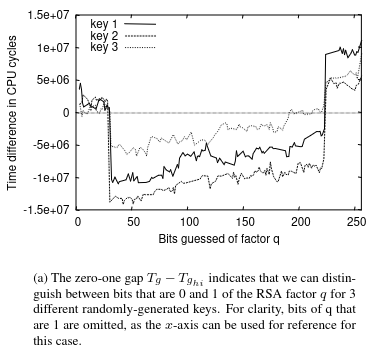
\includegraphics[height=0.9\textheight]{../spectre/remote-timing-prac-fig3a}
    \imagecredit{Figure 3a from Brumley and Boneh, ``Remote Timing Attacks are Practical''}
\end{frame}


\subsection{example: which website}

\begin{frame}{browsers and website leakage}
    \begin{itemize}
    \item web browsers run code from untrusted webpages
    \item one goal: can't tell what other webpages you visit
    \end{itemize}
\end{frame}

\begin{frame}[fragile]{some webpage leakage (1)}
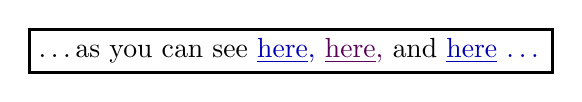
\begin{tikzpicture}
\node[draw,very thick] {
    \ldots as you can see \color{blue!70!black}{\underline{here}}, \color{violet!70!black}{\underline{here}},
    \color{black!70!black}{and} \color{blue!70!black}{\underline{here}} \ldots
};
\end{tikzpicture}
\begin{itemize}
\item convenient feature 1: browser marks visited links
\end{itemize}
\begin{tikzpicture}
\node[draw,very thick,align=left] {
\begin{lstlisting}[style=smaller,language={}]
<script>
var the_color = window.getComputedStyle(
    document.querySelector('a[href=~"foo.com"]')
).color
if (the_color == ...) { ... }
</script>
\end{lstlisting}
};
\end{tikzpicture}
\begin{itemize}
\item \sout<2->{convenient feature 2: scripts can query current color of something}
    \begin{itemize}
    \item<2-> fix 1: getComputedStyle lies about the color
    \item<2-> fix 2: limited styling options for visited links
    \end{itemize}
\end{itemize}
\end{frame}

\begin{frame}{some webpage leakage (2)}
\begin{itemize}
\item one idea: script in webpage times loop that writes big array
\item variation in timing depends on \myemph{other things running on machine}
\end{itemize}
\begin{tikzpicture}
\begin{visibleenv}<2->
\node (pic) {
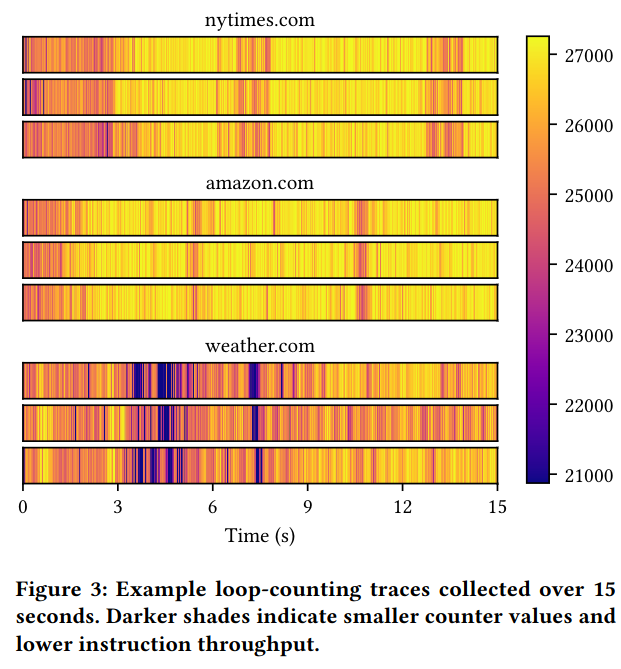
\includegraphics[height=0.6\textheight]{../spectre/website-sigs-fig}
};
\node[anchor=north west,align=left] at (pic.north east) {
turns out, other webpages \\
create distinct ``signatures'' \\
\fontsize{8}{9}\selectfont\parbox{10cm}{Figure from Cook et al, ``There’s Always a Bigger Fish:
Clarifying Analysis of a Machine-Learning-Assisted Side-Channel Attack'' (ISCA '22)}
};
\end{visibleenv}
\end{tikzpicture}
\end{frame}


% FIXME: \subsection{example: RF leaks}

% FIXME: \subsection{example: power analysis}

% FIXME: based on https://search.iczhiku.com/paper/U27SsPw1R1KrhDKc.pdf % Crypto'99 DPA paper

\section{cache side channels}

\subsection{introduction: observing cache evictions}

\begin{frame}{inferring cache accesses (1)}
\begin{itemize}
\item suppose I time accesses to array of chars:
    \begin{itemize}
    \item reading array[0]: 3 cycles
    \item reading array[64]: 4 cycles
    \item reading array[128]: 4 cycles
    \item reading array[192]: 20 cycles
    \item reading array[256]: 4 cycles
    \item reading array[288]: 4 cycles
    \item \ldots
    \end{itemize}
\item what could cause this difference?
    \begin{itemize}
    \item array[192] not in some cache, but others were
    \end{itemize}
\end{itemize}
\end{frame}

\begin{frame}[fragile,label=cacheAccess]{inferring cache accesses (2)}
some psuedocode:
\begin{lstlisting}[language=C,style=smaller]
char array[CACHE_SIZE];
AccessAllOf(array);
*other_address += 1;
TimeAccessingArray();
\end{lstlisting}
\begin{itemize}
\item suppose during these accesses I discover that
    \texttt{array[128]} is slower to access
\item probably because \texttt{*other\_address} loaded into cache + evicted it
\item what do we know about \texttt{other\_address}? (select all that apply)
\end{itemize}
\small
\begin{tabular}{lll}
A. same cache tag & B. same cache index & C. same cache offset \\
D. diff. cache tag & E. diff. cache index & F. diff. cache offset \\
\end{tabular}
\end{frame}


\begin{frame}{some complications}
    \begin{itemize}
    \item caches often use physical, not virtual addresses
        \begin{itemize}
        \item (and need to know about physical address to compare index bits)
        \item (but can infer physical addresses with measurements/asking OS)
        \item (often OS allocates contiguous physical addresses esp. w/`large pages')
        \end{itemize}
    \item storing/processing timings evicts things in the cache
        \begin{itemize}
        \item (but can compare timing with/without access of interest to check this)
        \end{itemize}
    \item processor ``pre-fetching'' may load things into cache before access is timed
        \begin{itemize}
            \item (but can arrange accesses to avoid triggering prefetcher \\
                and make sure to measure with memory barriers)
        \end{itemize}
    \item some L3 caches use a simple hash function to select index instead of  index bits
    \end{itemize}
\end{frame}


    % FIXME:
        % setup example 1:
            % fill cache; do something that accesses var part; time accessing everything --- slower if ___

\subsection{exercise: detect this access? (DM)}
\begin{frame}[fragile]{exercise: inferring cache accesses (1)}
\begin{lstlisting}[language=C,style=smaller]
char *array;
array = AllocateAlignedPhysicalMemory(CACHE_SIZE);
LoadIntoCache(array, CACHE_SIZE);
if (mystery) {
    *pointer += 1;
}
if (TimeAccessTo(&array[index]) > THRESHOLD) {
    /* pointer accessed */
}
\end{lstlisting}
\begin{itemize}
    \item suppose \texttt{pointer} is \texttt{0x1000188}
\item and cache (of interest) is direct-mapped, 32768 ($2^{15}$) byte, 64-byte blocks
\item what array index should we check?
\end{itemize}
\end{frame}

\begin{frame}<0>[label=inferCache1Soln,fragile]{solution}
\begin{lstlisting}[language=C,style=script]
array = AllocateAlignedPhysicalMemory(CACHE_SIZE);
LoadIntoCache(array, CACHE_SIZE);
if (mystery) { *pointer = 1; }
if (TimeAccessTo(&array[index]) > THRESHOLD) { /* pointer accessed */ }
\end{lstlisting}
\begin{itemize}
    \item $2^{15}$ byte direct mapped cache, $64=2^{6}$ byte blocks
    \item \myemph<2>{9 index bits}, 6 offset bits
    \item \texttt{0x1000188}: \texttt{\ldots 0\myemph<2>{\textit{000 0001 10}}00 1000}
    \vspace{.5cm}
    \item \texttt{array[0]} starts at multiple of cache size --- index 0, offset 0
    \item to get index 6, offset 0 array[\texttt{0b\myemph{\textit{1 10}}00 0000}] = array[\texttt{0x180}]
\end{itemize}
\end{frame}

\iftoggle{heldback}{}{\againframe<1->{inferCache1Soln}}

\begin{frame}[label=inferCache1Aside,fragile]{aside}
\begin{lstlisting}[language=C,style=smaller]
array = AllocateAlignedPhysicalMemory(CACHE_SIZE);
LoadIntoCache(array, CACHE_SIZE);
if (mystery) { *pointer += 1; }
if (TimeAccessTo(&array[index]) > THRESHOLD) {
    /* pointer accessed */
}
\end{lstlisting}
\begin{itemize}
    \item will this detect when pointer accessed? yes
    \item will this detect if mystery is true? not quite
    \item \ldots because branch prediction could started cache access
\end{itemize}
\end{frame}


\begin{frame}[fragile]{exercise: inferring cache accesses (2)}
\begin{lstlisting}[language=C,style=smaller]
char *other_array = ...;
char *array;
array = AllocateAlignedPhysicalMemory(CACHE_SIZE);
LoadIntoCache(array, CACHE_SIZE);
other_array[mystery] += 1;
for (int i = 0; i < CACHE_SIZE; i += BLOCK_SIZE) {
    if (TimeAccessTo(&array[i]) > THRESHOLD) {
        /* found something interesting */
    }
}
\end{lstlisting}
\begin{itemize}
\item other\_array at 0x200400, and interesting index is i=0x800,
    then what was mystery?
\end{itemize}
\end{frame}

\begin{frame}<0>[label=inferCache2Soln,fragile]{solution}
\begin{lstlisting}[language=C,style=script]
array = AllocateAlignedPhysicalMemory(CACHE_SIZE);
LoadIntoCache(array, CACHE_SIZE);
other_array[mystery] += 1;
for (int i = 0; i < CACHE_SIZE; i += BLOCK_SIZE) {
    if (TimeAccessTo(&array[i]) > THRESHOLD) { ... }
}
\end{lstlisting}
\begin{itemize}
    \item at i=0x800: \texttt{\ldots 0\myemph{\textit{000 1000 00}}00 0000} (cache index = 0x20)
    \item other\_array at \texttt{0x200400}
    \item Q: \texttt{0x200400 + X} has cache index 0x20? 
\end{itemize}
{\tt\small
\begin{tabular}{l|lll}
0x200400 & \ldots 0 & \myemph{000 0100 00} & 00 0000 \\
+ X      & \ldots ? & \myemph{000 0100 00} & ?? ???? \\ \hline
    0x200400+X & \ldots ? & \myemph{000 1000 00} & ?? ???? \\
\end{tabular}
}
\end{frame}

\iftoggle{heldback}{}{\againframe<1->{inferCache2Soln}}

\subsection{exercise: detect this access? (2-way)}


\begin{frame}[fragile]{exercise: inferring cache accesses (2)}
\begin{lstlisting}[language=C,style=smaller]
char *array;
posix_memalign(&array, CACHE_SIZE, CACHE_SIZE);
LoadIntoCache(array, CACHE_SIZE);
if (mystery) {
    *pointer = 1;
}
if (TimeAccessTo(&array[index1]) > THRESHOLD ||
    TimeAccessTo(&array[index2]) > THRESHOLD) {
    /* pointer accessed */
}
\end{lstlisting}
\begin{itemize}
\item pointer is 0x1000188
\item cache is 2-way, 32768 ($2^{15}$) byte, 64-byte blocks, ???? replacement
\item what array indexes should we check?
\end{itemize}
\end{frame}


\subsection{PRIME+PROBE, AES example}
\begin{frame}{PRIME+PROBE}
    \begin{itemize}
    \item name in literature: PRIME + PROBE
    \item PRIME: fill cache (or part of it) with values
    \item do thing that uses cache
    \item PROBE: access those values again and see if it's slow
    \vspace{.5cm}
    \item (one of several ways to measure how cache is used)
    \vspace{.5cm}
    \item coined in attacks on AES encryption
    \end{itemize}
\end{frame}

\begin{frame}{example: AES (1)}
\begin{itemize}
\item from Osvik, Shamir, and Tromer, ``Cache Attacks and Countermeasures: the Case of AES'' (2004)
\item early AES implementation used lookup table
\item goal: detect index into lookup table
    \begin{itemize}
    \item index depended on key + data being encrypted
    \end{itemize}
\item tricks they did to make this work
    \begin{itemize}
    \item vary data being encrypted
    \item subtract average time to look for what changes
    \item lots of measurements
    \end{itemize}
\end{itemize}
\end{frame}

\begin{frame}{example: AES (2)}
\small from Osvik, Shamir, and Tromer, ``Cache Attacks and Countermeasures: the Case of AES'' (2004) \\
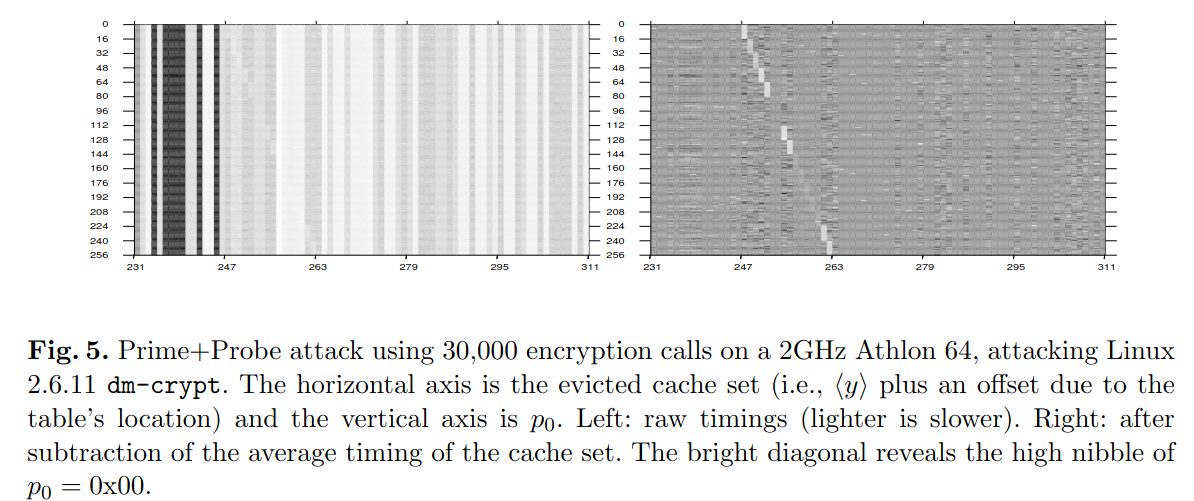
\includegraphics[width=1.0\textwidth]{../spectre/prime-probe-osvik}
\end{frame}
 % FIXME: lfence-using example

\subsection{reading a value (1)}
\begin{frame}[fragile]{reading a value}
\begin{lstlisting}[language=C,style=smaller]
char *array;
posix_memalign(&array, CACHE_SIZE, CACHE_SIZE);
AccessAllOf(array);
other_array[mystery * BLOCK_SIZE] += 1;
for (int i = 0; i < CACHE_SIZE; i += BLOCK_SIZE) {
    if (CheckIfSlowToAccess(&array[i])) {
        ...
    }
}
\end{lstlisting}
\begin{itemize}
\item with 32KB direct-mapped cache
\item suppose we find out that \texttt{array[0x400]} is slow to access
\item and other\_array starts at address 0x100000
\item what was mystery?
\end{itemize}
\end{frame}


\section{seeing speculation via side channels}

\subsection{revising array lookup}

\usetikzlibrary{matrix}
\begin{frame}[fragile]{revisiting an earlier example (1)}
\begin{lstlisting}[language=C,style=smaller]
char *array;
posix_memalign(&array, CACHE_SIZE, CACHE_SIZE);
LoadIntoCache(array, CACHE_SIZE);
if (mystery) {
    *pointer += 1;
}
if (TimeAccessTo(&array[index]) > THRESHOLD) {
    /* pointer accessed */
}
\end{lstlisting}
\begin{itemize}
\item what if mystery is false \textit{but} branch mispredicted?
\end{itemize}
\end{frame}

\begin{frame}[fragile]{revisiting an earlier example (2)}
\lstset{language=myasm}
\begin{tikzpicture}
\tikzset{
    forwardLine/.style={blue!60!black,thick,-Latex},
    hiForwardOn/.style={alt=#1{blue}{}},
    forwardLineB/.style={red,dashed,thick,-Latex},
    sepLine/.style={black!40,densely dotted},
};
\tikzset{
    fetch/.style={fill=red!15},
    decode/.style={fill=orange!15},
    rename/.style={fill=yellow!15},
    issue/.style={fill=yellow!15!green!15},
    execute/.style={fill=blue!15},
    memory/.style={fill=blue!15},
    writeback/.style={fill=violet!15},
    commit/.style={fill=magenta!20},
}
\newcommand{\fdemw}{ \& |[fetch]| F \& |[decode]| D \& |[rename]| R \& |[issue]| I \& |[execute]| E \& |[memory]| M \& |[writeback]| W}
\newcommand{\fdew}{ \& |[fetch]| F \& |[decode]| D \& |[rename]| R \& |[issue]| I \& |[execute]| E \& |[writeback]| W}
\newcommand{\fdr}{ \& |[fetch]| F \& |[decode]| D \& |[rename]| R}
\newcommand{\issw}{ \& |[issue]| I \& |[execute]| E \& |[writeback]| W}
\newcommand{\fdem}{ \& |[fetch]| F \& |[decode]| D \& |[rename]| R \& |[issue]| I \& |[execute]| E \& |[memory]| M }
\newcommand{\m}{ \& |[memory]| M }
\newcommand{\w}{ \& |[writeback]| W }
\newcommand{\rn}{ \& |[rename]| R }
\newcommand{\iss}{ \& |[issue]| I }
\newcommand{\cmt}{ \& |[commit]| C }
\newcommand{\dec}{ \& |[decode]| D } % conflicts with existing \d macro
\newcommand{\e}{ \& |[execute]| E }
\newcommand{\f}{ \& |[fetch]| F }
\matrix[tight matrix no line,
        nodes={text width=.6cm,inner sep=0mm,outer sep=0mm},
        column sep={.6cm,between origins},
        row sep={.7cm,between origins},
        column 1/.style={nodes={font=\tt,text width=6cm,align=left},column sep=0cm},
        ] (tbl) {
|[align=right]| \normalfont\textit{cycle \#} \hspace{.5cm}
                                 \& 0 \& 1 \& 2 \& 3 \& 4 \& 5 \& 6 \& 7 \& 8 \& 9 \& 10 \& 11\\
movq mystery, \%rax   \fdr \iss \e\e\e \w \cmt \\
test \%rax, \%rax      \fdr \& ~ \& ~ \& \issw \cmt\\
jz skip {\normalfont (mispred.) }    \& ~ \fdr \& ~ \& ~ \& ~ \issw \cmt \\
mov pointer, \%rax      \& ~ \fdr \iss \e\e\e \w \& \\
mov (\%rax), \%r8 \& ~ \& ~ \fdr \& ~ \& ~ \& ~ \issw \& \\
add \$1, \%r8     \& ~ \& ~ \fdr \\
mov \%r8, \%rax   \& ~ \& ~ \& ~ \fdr \\
\ldots \\
skip: ...       \& ~ \& ~ \& ~ \& ~ \& ~ \& ~ \&~ \fdr \\
};
% FIXME: hilite in-order and out-of-order parts of pipeline
\tikzset{
    hibox/.style={draw=red,ultra thick,inner sep=0mm},
    text box/.style={fill=white,draw=red, ultra thick,align=left},
}
\end{tikzpicture}
\end{frame}

\begin{frame}[fragile]{avoiding/triggering this problem}
\begin{lstlisting}[language=C,style=smaller]
if (something false) {
    access *pointer;
}
\end{lstlisting}
\begin{itemize}
\item what can we do to make access more/less likely to happen?
\end{itemize}
\end{frame}

 

% FIXME: piepline
\subsection{reading a value (2)}
\begin{frame}<1>[label=readWithoutRead,fragile]{reading a value without really reading it}
\begin{lstlisting}[language=C,style=smaller]
char *array;
posix_memalign(&array, CACHE_SIZE, CACHE_SIZE);
AccessAllOf(array);
if (something false) {
    other_array[mystery * BLOCK_SIZE] += 1;
}
for (int i = 0; i < CACHE_SIZE; i += BLOCK_SIZE) {
    if (CheckIfSlowToAccess(&array[i])) {
        ...
    }
}
\end{lstlisting}
\begin{itemize}
\item if branch mispredicted, cache access may \myemph{still happen}
\item can find the value of \texttt{mystery}
\end{itemize}
\end{frame}


\section{meltdown}

\subsection{well, what else gets speculated?}
\begin{frame}[fragile]{seeing past a segfault? (1)}
\begin{lstlisting}[language=C,style=small]
Prime();
if (something false) {
    triggerSegfault();
    Use(*pointer);
}
Probe();
\end{lstlisting}
\begin{itemize}
\item could cache access for \texttt{*pointer} still happen?
\item yes, if:
    \begin{itemize}
    \item branch for if statement mispredicted, and
    \item \texttt{*pointer} starts before segfault detected
    \end{itemize}
\end{itemize}
\end{frame}

\begin{frame}[fragile]{seeing past a segfault? (2)}
\begin{itemize}
\item operations in virtual memory lookup:
    \begin{itemize}
    \item translate virtual to physical address
    \item check if access is permitted by permission bits
    \end{itemize}
\item Intel processors: looks like these were separate steps, so...
\end{itemize}
\lstset{
    language=C,
    style=small,
    moredelim=**[is][\btHL<1|handout:1>]{@1}{@},
    moredelim=**[is][\btHL<2|handout:2>]{@2}{@},
    moredelim=**[is][\btHL<3|handout:3>]{@3}{@},
    moredelim=**[is][\btHL<4|handout:4>]{@4}{@},
}
\begin{lstlisting}
Prime();
if (@2something false@) {
    int value = @3ReadMemoryMarkedNonReadableInPageTable();@
    access other_array[value @4* ...@];
}
Probe();
\end{lstlisting}
\end{frame}


\subsection{vulnerability}
\begin{frame}[fragile]{Meltdown}

{\small from Lipp et al, ``Meltdown: Reading Kernel Memory from User Space''} \\
\lstset{
    language=myasm,
    style=small,
    moredelim={**[is][\btHL<2>]{@2}{2@}},
    moredelim={**[is][\btHL<3>]{@3}{3@}},
    moredelim={**[is][\btHL<4>]{@4}{4@}},
    moredelim={**[is][\btHL<5>]{@5}{5@}},
}
\begin{lstlisting}
    // %rcx = kernel address
    // %rbx = array to load from to cause eviction
    xor %rax, %rax      // rax <- 0
retry:
    // rax <- memory[kernel address] (segfaults)
    // but check for segfault done out-of-order on Intel at time
    @5movb (%rcx), %al5@
    // rax <- memory[kernel address] * 4096 [speculated]
    @2shl $0xC, %rax2@
    @3jz retry3@            // not-taken branch
    // access array[memory[kernel address] * 4096]
    @4mov (%rbx, %rax), %rbx4@
\end{lstlisting}
\begin{tikzpicture}[overlay,remember picture]
\coordinate (box place) at ([yshift=0.25cm]current page.center);
\tikzset{
    box/.style={at=(box place), anchor=south,align=left,fill=white,draw=red,ultra thick}
}
\begin{visibleenv}<2>
\node[box] {space out accesses by 4096 \\
ensure separate cache sets and \\
avoid triggering prefetcher
};
\end{visibleenv}
\begin{visibleenv}<3>
\node[box] {
    repeat access if zero \\
    apparently value of zero speculatively read \\
    when real value not yet available
};
\end{visibleenv}
\begin{visibleenv}<4>
\node[box] {
    access cache to allow measurement later \\
    in paper with FLUSH+RELOAD instead \\\
    of PRIME+PROBE technique
};
\end{visibleenv}
\begin{visibleenv}<5>
\node[box] {
    segfault actually happens eventually \\
    option 1: okay, just start a new process every time \\
    option 2: way of suppressing exception (transactional memory support)
};
\end{visibleenv}
\end{tikzpicture}
\end{frame}



\subsection{fix}

\begin{frame}{Meltdown fix}
\begin{itemize}
\item HW: permissions check done with/before physical address lookup
    \begin{itemize}
    \item was already done by AMD, ARM apparently?
    \item now done by Intel
    \end{itemize}
\item SW: separate page tables for kernel and user space
    \begin{itemize}
    \item don't have sensitive kernel memory pointed to by page table \\
        when user-mode code running
    \item unfortunate performance problem
    \item exceptions start with code that switches page tables
    \end{itemize}
\end{itemize}
\end{frame}


\section{spectre}

\subsection{concept: forcing branch misprediction}
\againframe<2>{readWithoutRead}
\begin{frame}[fragile]{mistraining branch predictor?}
\begin{lstlisting}[language=C]
if (something) {
    CodeToRunSpeculatively()
}
\end{lstlisting}
\begin{itemize}
\item how can we have `something' be false, but predicted
    as true
\vspace{.5cm}
\item run lots of times with something true
\item then do actually run with something false
\end{itemize}
\end{frame}



\subsection{contrived? vulnerable code}
\begin{frame}[fragile]{contrived(?) vulnerable code (1)}
\begin{itemize}
\item suppose this C code is run with extra privileges
    \begin{itemize}
    \item (e.g. in system call handler, library called from JavaScript in webpage, etc.)
    \end{itemize}
\item assume \texttt{x} chosen by attacker
\item (example from original Spectre paper)
\end{itemize}
\begin{lstlisting}
if (x < array1_size)
        y = array2[array1[x] * 4096];
\end{lstlisting}
\end{frame}

\begin{frame}[fragile]{the out-of-bounds access (1)}
\begin{lstlisting}
char array1[...];
...
int secret;
...
y = array2[array1[x] * 4096];
\end{lstlisting}
\begin{itemize}
\item suppose array1 is at \texttt{0x1000000} and
\item secret is at \texttt{0x103F0003};
\item what x do we choose to make \lstinline|array1[x]| access first byte of secret?
\end{itemize}
\end{frame}

\begin{frame}[fragile]{the out-of-bounds access (2)}
\begin{lstlisting}
char array1[...];
...
int secret;
...
y = array2[array1[x] * 4096];
\end{lstlisting}
\begin{itemize}
\item suppose our cache has 64-byte blocks and 8192 sets
\item and \lstinline|array2[0]| is stored in cache set 0
\vspace{.5cm}
\item if the above evicts something in cache set 128, \\
      then what do we know about \texttt{array1[x]}?
    \begin{itemize}
    \item<2-> is 2 or 254
    \end{itemize}
\end{itemize}
\end{frame}

\begin{frame}[fragile]{exploit with contrived(?) code}
\begin{lstlisting}[language=C,style=smaller]
/* in kernel: */
int systemCallHandler(int x) {
    if (x < array1_size)
        y = array2[array1[x] * 4096];
    return y;
}
\end{lstlisting}
\hrule
\begin{lstlisting}[language=C,style=smaller]
/* exploiting code */
    /* step 1: mistrain branch predictor */
for (a lot) {
    systemCallHandler(0 /* less than array1_size */);
}
    /* step 2: evict from cache using misprediction */
Prime();
systemCallHandler(targetAddress - array1Address);
int evictedSet = ProbeAndFindEviction();
int targetValue = (evictedSet - array2StartSet) / setsPer4K;
\end{lstlisting}
\end{frame}


\subsection{array bounds check}
\begin{frame}[fragile]{really contrived?}
\begin{lstlisting}[language=C,style=smaller]
char *array1; char *array2;
if (x < array1_size)
    y = array2[array1[x] * 4096];
\end{lstlisting}
\begin{itemize}
\item times 4096 shifts so we can get lower bits of target value
    \begin{itemize}
    \item so all bits effect what cache block is used
    \end{itemize}
\end{itemize}
\hrule
\begin{visibleenv}<2->
\begin{lstlisting}[language=C,style=smaller]
int *array1; int *array2;
if (x < array1_size)
    y = array2[array1[x]];
\end{lstlisting}
\begin{itemize}
\item will still get \textit{upper} bits of array1[x] (can tell from cache set)
\item<2-> can still read arbitrary memory!
    \begin{itemize}
    \item want memory at 0x10000?
    \item upper bits of 4-byte integer at 0x3FFFE
    \end{itemize}
\end{itemize}
\end{visibleenv}
\end{frame}

\begin{frame}[fragile]{bounds check in kernel}
\lstset{
    language=C,
    style=small,
    moredelim={**[is][\btHL<2>]{@2}{2@}},
    moredelim={**[is][\btHL<3>]{@3}{3@}},
    moredelim={**[is][\btHL<4>]{@4}{4@}},
    moredelim={**[is][\btHL<5>]{@5}{5@}},
}
\begin{tikzpicture}
\node[draw,very thick,text width=10cm,label={east:actual code}] (syscall) {
\begin{lstlisting}
void SomeSystemCallHandler(int index) {
    if (@2index > some_table_size2@) 
        return ERROR;
    int kind = @3table[index]3@;
    switch (@4other_table[kind].foo4@) {
        ...
    }
}
\end{lstlisting}
};
\node[draw,very thick,anchor=south west,text width=10cm,label={east:our template}] (template) at (syscall.north west) {
\begin{lstlisting}
if (@2x < array1_size2@) {
    y = @4array2[@3array1[x]3@]4@);
}
\end{lstlisting}
};
\end{tikzpicture}
\end{frame}


\subsection{JavaScript exploit}
\begin{frame}{privilege levels?}
    \begin{itemize}
    \item vulnerable code runs with higher privileges
    \item so far: higher privileges = kernel mode
    \vspace{.5cm}
    \item but other common cases of higher privileges
    \item example: scripts in web browsers
    \end{itemize}
\end{frame}

\begin{frame}[fragile]{JavaScript}
\begin{itemize}
\item JavaScript: scripts in webpages
\item not supposed to be able to read arbitrary memory, but\ldots
\item can access arrays to examine caches
\item and could take advantage of some browser function being vulnerable
\vspace{.5cm}
\item<2-> or --- \myemph<2>{doesn't even need browser to supply vulnerable code itself!}
\end{itemize}
\end{frame}

\begin{frame}[fragile]{just-in-time compilation?}
\begin{itemize}
\item for performance, compiled to machine code, run in browser
\item not supposed to be access arbitrary browser memory
\item example JavaScript code from paper:
\end{itemize}
\begin{lstlisting}[language=JavaScript,style=small]
if (index < simpleByteArray.length) {
    index = simpleByteArray[index | 0];
    index = (((index * 4096)|0) & (32*1024*1024-1))|0;
    localJunk ˆ= probeTable[index|0]|0;
}
\end{lstlisting}
\begin{itemize}
\item web page runs a lot to train branch predictor
\item then does run with out-of-bounds index
\item examines what's evicted by probeTable access
\end{itemize}
\end{frame}


\subsection{mispredicted indirect}
\begin{frame}[fragile]{other misprediction}
\begin{itemize}
\item so far: talking about mispredicting direction of branch
\item what about mispredicting target of branch in, e.g.:
\end{itemize}
\begin{lstlisting}
// possibly from C code like:
//   (*function_pointer)();
jmp *%rax           

// possibly from C code like:
//      switch(rcx) { ... }
jmp *(%rax,%rcx,8)  
\end{lstlisting}
\end{frame}

\begin{frame}[fragile]{an idea for predicting indirect jumps}

for jmps like \lstinline|jmp *%rax| predict target with cache: \\
\begin{tabular}{ll}
bottom 12 bits of jmp address & last seen target \\ \hline
0x0--0x7 & 0x200000 \\
0x8--0xF & 0x440004 \\
0x10-0x18 & 0x4CD894 \\
0x18-0x20 & 0x510194 \\
0x20-0x28 & 0x4FF194 \\
\ldots & \ldots \\
0xFF8--0xFFF & 0x3F8403 \\
\end{tabular}
\begin{itemize}
\item Intel Haswell CPU did something similar to this
    \begin{itemize}
    \item uses bits of last several jumps, not just last one
    \end{itemize}
\item can mistrain this branch predictor
\end{itemize}
\end{frame}

\begin{frame}[fragile]{using mispredicted jump}
\begin{itemize}
\item 1: find some kernel function with \lstinline|jmp *%rax|
\item 2: mistrain branch target predictor for it to jump to chosen code
    \begin{itemize}
    \item use code at address that conflicts in ``recent jumps cache''
    \end{itemize}
\item 3: have chosen code be attack code (e.g. array access)
    \begin{itemize}
    \item either write special code OR
    \item find suitable instructions (e.g. array access) in existing kernel code
    \end{itemize}
\end{itemize}
\end{frame}



\subsection{more variants?}
\begin{frame}{Spectre variants}
    \begin{itemize}
    \item showed Spectre variant 1 (array bounds), 2 (indirect jump)
        \begin{itemize}
        \item from original paper
        \end{itemize}
    \vspace{.5cm}
    \item other possible variations:
        \begin{itemize}
        \item could cause other things to be mispredicted
            \begin{itemize}
            \item prediction of where functions return to?
            \item values instead of which code is executed?
            \end{itemize}
        \item could use side-channel other than data cache changes
            \begin{itemize}
            \item instruction cache
            \item cache of pending stores not yet committed
            \item contention for resources on multi-threaded CPU core
            \item branch prediction changes
            \item \ldots
            \end{itemize}
        \end{itemize}
    \end{itemize}
\end{frame}


\subsection{software fix}
\begin{frame}[fragile]{some Linux kernel mitigations (1)}
\begin{itemize}
\item replace \lstinline|array[x]| with \lstinline|array[x & ComputeMask(x, size)]|
\item \ldots where ComputeMask() returns
    \begin{itemize}
    \item 0 if x $>$ size
    \item \texttt{0xFFFF..F} if x $\le$ size
    \end{itemize}
\item \ldots and ComputeMask() does not use jumps:
\end{itemize}
\begin{lstlisting}[style=small,language=myasm]
mov x, %r8
mov size, %r9
cmp %r9, %r8
sbb %rax, %rax  // sbb = subtract with borrow
    // either 0 or -1
\end{lstlisting}
\end{frame}

\begin{frame}[fragile]{some Linux kernel mitigations (2)}
\begin{itemize}
\item for indirect branches:
\vspace{.5cm}
\item with hardware help:
    \begin{itemize}
    \item separate indirect (computed) branch prediction for kernel v user mode
    \item other branch predictor changes to isolate better
    \end{itemize}
\item without hardware help:
    \begin{itemize}
    \item transform \lstinline|jmp *(%rax)|, etc. into code that \\
        will only predicted to jump to safe locations \\
        (by writing assembly very carefully)
    \end{itemize}
\end{itemize}
\end{frame}

\begin{frame}[fragile]{only safe prediction}
\begin{itemize}
\item as replacement for \lstinline|jmp *(%rax)|
\item code from Intel's ``Retpoline: A Branch Target Injection Mitigation''
\end{itemize}
\begin{lstlisting}[language=myasm,style=small]
        call load_label
    capture_ret_spec:       /* <-- want prediction to go here */
        pause
        lfence
        jmp capture_ret_spec
    load_label:
        mov %rax, (%rsp)
        ret
\end{lstlisting}
\end{frame}


\section{backup slides}
\begin{frame}{backup slides}
\end{frame}


\section{backup slides}
\begin{frame}{backup slides}
\end{frame}



\subsection{predicting targets}
\usetikzlibrary{matrix}

\begin{frame}{branch target buffer}
    \begin{itemize}
    \item what if we can't decode LABEL from machine code for \texttt{jmp LABEL} or \texttt{jle LABEL} fast?
        \begin{itemize}
        \item will happen in more complex pipelines
        \end{itemize}
    \item what if we can't decode that there's a RET, CALL, etc. fast?
    \end{itemize}
\end{frame}

\begin{frame}[fragile,label=btbStructure]{BTB: cache for branch targets}
\begin{tikzpicture}
\tikzset{
    marked idx/.style={fill=blue!15},
    marked tag/.style={fill=green!15},
    marked target/.style={fill=cyan!15},
}
\matrix[
    tight matrix,
    nodes={font=\fontsize{9}{10}\tt\selectfont},
    row 1/.append style={nodes={font=\bfseries\fontsize{9}{10}\selectfont}},
    column 1/.style={nodes={text width=1cm,draw=none}},
    column 2/.style={nodes={text width=0.8cm}},
    column 3/.style={nodes={text width=1.5cm}},
    column 4/.style={nodes={text width=0.8cm}},
    column 5/.style={nodes={text width=2cm}},
    column 6/.style={nodes={text width=3cm}},
    column 7/.style={nodes={text width=2cm}},
    column 8/.style={nodes={text width=0.25cm,draw=none}},
    column 9/.style={nodes={text width=0.8cm}},
] (btb) at (0, 0) {
    idx \& valid \& tag \& ofst \& type \& target \& (more info?) \& ~ \& valid \& \ldots\\
    |[alt=<3>{marked idx}]| 0x00 \& 1 \& |[alt=<3>{marked tag}]| 0x400 \& |[alt=<3>{marked tag}]| 5 \& Jxx \& |[alt=<3>{marked target}]| 0x3FFFF3 \& \ldots \& ~ \& 1 \& \ldots\\
    0x01 \& 1 \& 0x401 \& C \& JMP \& 0x401035 \& --- \& ~ \& 0 \& \ldots \\
    0x02 \& 0 \& --- \& ---\& --- \& --- \& ---  \& ~ \& 0 \&\ldots \\
    0x03 \& 1 \&  0x400 \& 9 \& RET \& --- \& \ldots \& ~ \& 0 \&\ldots\\
    \ldots \& \ldots \& \ldots \& \ldots \& \ldots \& \ldots \& \ldots \& ~ \& \ldots \& \ldots \\
    |[alt=<2>{marked idx}]| 0xFF \& 1 \& |[alt=<2>{marked tag}]| 0x3FF \& |[alt=<2>{marked tag}]| 8 \& CALL \& |[alt=<2>{marked target}]| 0x404033 \& \ldots \& ~ \& 0 \& \ldots \\
};
\matrix[tight matrix,
    nodes={font=\fontsize{9}{10}\tt\selectfont},
    column 1/.style={nodes={text width=2cm,draw=none}},
    column 2/.style={nodes={text width=8cm,draw=none}},
    anchor=north west,
] at ([yshift=-1cm]btb.south west) {
    0x3FFFF3: \& movq \%rax, \%rsi \\
    0x3FFFF7: \& pushq \%rbx\\
    \alt<2>{\fboxsep=0pt0x\colorbox{green!15}{3FF}\colorbox{blue!15}{FF}\colorbox{green!15}{8}}{0x3FFFF8}: \& call \alt<2>{\fboxsep0pt\colorbox{cyan!15}{0x404033}}{0x404033} \\
    0x400001: \& popq \%rbx \\
    0x400003: \& cmpq \%rbx, \%rax \\
    \alt<3>{\fboxsep=0pt0x\colorbox{green!15}{400}\colorbox{blue!15}{00}\colorbox{green!15}{5}}{0x400005}: \& jle \alt<3>{\fboxsep0pt\colorbox{cyan!15}{0x3FFFF3}}{0x3FFFF3} \\
    \ldots \& \ldots \\
    0x400031:  \& ret \\
    \ldots \& \ldots \\
};
\end{tikzpicture}
\end{frame}

\begin{frame}{indirect branch prediction}
    \begin{itemize}
        \item for instructions like: \texttt{jmp *\%rax} or \texttt{jmp *(\%rax, \%rcx, 8)}
        \item simple idea: record what happened last time, predict the same
        \item example: Intel's Haswell strategy:
        \vspace{.5cm}
        \item maintain hash of last several jump instruction addresses
        \item lookup hash in table of targets
        \item use result as prediction, update if prediction wrong
    \end{itemize}
\end{frame}


\subsection{predicting returns}
\usetikzlibrary{arrows.meta,matrix,positioning}

\begin{frame}{predicting ret: ministack of return addresses}
\begin{itemize}
    \item predicting ret --- ministack in processor registers
        \begin{itemize}
        \item push on ministack on call; pop on ret
        \end{itemize}
    \item ministack overflows? discard oldest, mispredict it later
\end{itemize}
\begin{tikzpicture}
\matrix [matrix of nodes, nodes={draw,rectangle,row sep=-\pgflinewidth,font=\scriptsize, text width=3cm},
         label={-90:stack in memory}] (realStack) {
    baz saved registers \\
    baz return address \\
    bar saved registers \\
    bar return address \\
    foo local variables \\
    foo saved registers \\
    foo return address \\
    foo saved registers \\
 };

\matrix [matrix of nodes,row sep=-\pgflinewidth,nodes={draw,rectangle,font=\scriptsize,text width=3cm},
         label={[align=center]-90:(partial?) stack\\in CPU registers},right=1cm of realStack] (fakeStack) {
    baz return address \\
    bar return address \\
    foo return address \\
 };
\end{tikzpicture}
\end{frame}

\begin{frame}{4-entry return address stack}
\begin{tikzpicture}
    \tikzset{>=Latex}
    \matrix[tight matrix,
        nodes={minimum height=.5cm},
        row 1/.style={nodes={minimum height=1.65cm}},
        column 2/.style={nodes={text width=3cm,draw}},
        column 1/.style={nodes={text width=1cm,draw}},
        label={north:4-entry return address stack in CPU},
    ] (ras) {
        idx \& {saved \\ return \\ addresses} \\
        0 \& 0x12345 \\
        1 \& 0x44432 \\
        2 \& 0x44F92 \\
        3 \& 0x22331 \\
    };
    \node[anchor=east,draw,label={[align=center]north:current\\index}] (ras idx) at ([xshift=-1cm]ras.west) {1};
\draw[very thick,->,dotted] (ras idx) -- ++(.5cm, 0cm) |- (ras-3-1.west);
    \draw[very thick,->] (ras-3-2.east) -- ++(2cm, 0cm) node[right ] {next prediction for ret};
    \draw[very thick,<-] (ras-4-2.east) -- ++(1cm, 0cm) -- ++(0cm, -1cm) node[below,align=center] {next saved \\ return address \\ from call};
\end{tikzpicture}
\begin{itemize}
\item on \texttt{call}: increment index, save return address in that slot
\item on \texttt{ret}: read prediction from index, decrement index
\end{itemize}
\end{frame}


\subsection{with local history}
\usetikzlibrary{arrows.meta,fit,matrix,positioning,shapes.callouts}

\begin{frame}{predict: repeat last}
\newcommand\showSelectionFrame{3-}
\newcommand\beforeShowSelectFrame{1-2}
\begin{tikzpicture}
\tikzset{
    >=Latex,
    connect/.style={draw,ultra thick},
}
% FIXME: PC --> hash function --> table
\node[draw,very thick,label={north:PC of branch},font=\tt] (pc) {0x4004\myemph<\showSelectionFrame>{2}A};
\node[anchor=north west,draw,very thick,fill=yellow!10,anchor=north west] (hash)
    at ([xshift=-.5cm,yshift=-1cm]pc.south east) {hash function};
\matrix[tight matrix,
    nodes={minimum height=.6cm},
    column 1/.style={nodes={
        draw=none,
        font=\small\tt,
        alt={<\showSelectionFrame>{text=black!50}},
    }},
    column 2/.style={nodes={text width=3.5cm,font=\small,alt=<\showSelectionFrame>{text=black!50,draw=black!50}}},
    row 1/.style={nodes={draw=none,text=black,font=\small\it,draw=none,minimum height=0.1cm}},
    row 4/.style={nodes={alt=<\showSelectionFrame>{text=black,fill=blue!10}}},
    row 4 column 2/.style={nodes={alt=<\showSelectionFrame>{draw=black,very thick}}},
    anchor=north west,
] (tbl) at ([xshift=4cm]pc.north east) {
    index \& {prediction/\\last result?} \\
    0 \& taken (1)\\
    1 \& not taken (0)\\
    2 \& taken (1) \\
    3 \& taken (1) \\
    |[draw=none]| \ldots \& |[draw=none]| \ldots \\
    14 \& not taken (0) \\
    15 \& taken (1) \\
};
\draw[connect,ultra thick,->] (pc.south) |- (hash.west);
\begin{visibleenv}<\beforeShowSelectFrame>
\draw[connect,dotted,black!50,ultra thick,->] (hash.east) -- ++(.4cm,0cm) |- (tbl-2-1.west);
\draw[connect,dotted,black!50,ultra thick,->] (hash.east) -- ++(.4cm,0cm) |- (tbl-3-1.west);
\draw[connect,dotted,black!50,ultra thick,->] (hash.east) -- ++(.4cm,0cm) |- (tbl-4-1.west);
\draw[connect,dotted,black!50,ultra thick,->] (hash.east) -- ++(.4cm,0cm) |- (tbl-5-1.west);
\draw[connect,dotted,black!50,ultra thick,->] (hash.east) -- ++(.4cm,0cm) |- (tbl-7-1.west);
\draw[connect,dotted,black!50,ultra thick,->] (hash.east) -- ++(.4cm,0cm) |- (tbl-8-1.west);
\end{visibleenv}
\begin{visibleenv}<\showSelectionFrame>
\draw[connect,ultra thick,->] (hash.east) -- ++(.4cm,0cm) |- (tbl-4-1.west);
\end{visibleenv}
\begin{visibleenv}<2>
\coordinate (callout hash loc) at ([xshift=-.5cm]hash.south);
\node[my callout2=callout hash loc,align=left,anchor=north] at ([xshift=2cm,yshift=-2cm]hash.south) {
    typical choice: some bits of branch address \\
    for our example: will use bits 4-7
};
\end{visibleenv}
\begin{visibleenv}<4->
\draw[connect,->,alt=<4>{red}] ([yshift=-.2cm]tbl-4-2.east) -- ++(1cm,0cm) -- ++(0cm,-3cm) node[below,align=center] {
    prediction \\
    to fetch stage
};
\end{visibleenv}
\begin{visibleenv}<5->
\draw[connect,<-,alt=<5>{red}] ([yshift=.2cm]tbl-4-2.east) -- ++(1cm,0cm) -- ++(0cm,1.5cm) node[above,align=center] {
    actual outcome \\
    (from later stage)
};
\end{visibleenv}
\end{tikzpicture}
\end{frame}

\begin{frame}[fragile,label=1bitPredExample]{example}
\newcommand\showSelectionFrame{1-}
\begin{tikzpicture}
\tikzset{
    >=Latex,
    connect/.style={draw,ultra thick},
}
\node[draw,very thick,label={north:PC of branch},font=\tt] (pc) {0x4004\myemph<\showSelectionFrame>{2}A};
\node[anchor=north west,draw,very thick,fill=yellow!10,anchor=north west] (hash)
    at ([xshift=-.5cm,yshift=-1cm]pc.south east) {hash function};
\matrix[tight matrix,
    nodes={minimum height=.6cm},
    column 1/.style={nodes={
        draw=none,
        font=\small\tt,
        alt={<\showSelectionFrame>{text=black!50}},
        text width=0.5cm
    }},
    column 2/.style={nodes={text width=4cm,font=\small,alt=<\showSelectionFrame>{text=black!50,draw=black!50}}},
    row 1/.style={nodes={draw=none,text=black,font=\small\it,draw=none,minimum height=0.1cm}},
    row 4/.style={nodes={alt=<\showSelectionFrame>{text=black,fill=blue!10}}},
    row 4 column 2/.style={nodes={alt=<\showSelectionFrame>{draw=black,very thick}}},
    anchor=north west,
] (tbl) at ([xshift=4cm]pc.north east) {
    idx \& {prediction/\\last result?} \\
    0 \& taken (1)\\
    1 \& not taken (0)\\
    2 \& \alt<1-4>{not taken (0)}{\sout{not taken}~\myemph<5>{taken (1)}} \\
    3 \& taken (1) \\
    |[draw=none]| \ldots \& |[draw=none]| \ldots \\
    14 \& not taken (0) \\
    15 \& taken (1) \\
};
\draw[connect,ultra thick,->] (pc.south) |- (hash.west);
\begin{visibleenv}<\showSelectionFrame>
\draw[connect,ultra thick,->] (hash.east) -- ++(.4cm,0cm) |- (tbl-4-1.west);
\end{visibleenv}
\matrix[tight matrix,anchor=north west,
    column 1/.style={nodes={font=\fontsize{10}{11}\selectfont\tt,text width=2cm}},
    column 2/.style={nodes={font=\fontsize{10}{11}\selectfont\tt,text width=3cm}},
] (code) at ([yshift=-.5cm,xshift=-3cm]hash.south west) {
0x40041B \& movq \$4, \%rax \\
|[alias=the target]| 0x400423 \& ... \\
0x400429 \& decq \%rax \\
|[alias=the branch]| 0x40042A \& jnz 0x400423 \\
0x40042B \& ... \\
};
\draw[dotted,thick,->] (the branch.west) -- ++(-.2cm,0cm) |- (the target.west);
\draw[connect,->,alt={<4,6,8>{red}}] ([yshift=-.2cm]tbl-4-2.east) -- ++(1cm,0cm) -- ++(0cm,-3cm) node[below,align=center] {
    prediction \\
    to fetch stage
};
\draw[connect,<-,alt={<5,7,9>{red}}] ([yshift=.2cm]tbl-4-2.east) -- ++(1cm,0cm) -- ++(0cm,1.5cm) node[above,align=center] {
    actual outcome \\
    from later stage
};
\begin{visibleenv}<2>
\node[fit=(code),inner sep=0mm,draw=red,ultra thick,
    label={[draw=red,align=left,fill=white,font=\small,xshift=2cm]south:%
    {assembly version of:\\\texttt{i = 4; do \{ ...; i -= 1; \} while (i)}}}] {};
\end{visibleenv}
\begin{visibleenv}<3->
% FIXME: chart of iteration #: prediction | outcome
\matrix[tight matrix,
    nodes={minimum height=.45cm,fill=white},
    column 1/.style={nodes={text width=1.8cm,font=\small}},
    column 2/.style={nodes={text width=2cm,font=\small}},
    column 3/.style={nodes={text width=2cm,font=\small}},
    row 3/.style={nodes={alt=<1-5>{invisible}}},
    row 4/.style={nodes={alt=<1-7>{invisible}}},
    row 5/.style={nodes={alt=<1-7>{invisible}}},
    row 6/.style={nodes={alt=<1-7>{invisible}}},
    row 7/.style={nodes={alt=<1-7>{invisible}}},
    row 8/.style={nodes={alt=<1-7>{invisible}}},
    anchor=north west
] at (code.east) {
iteration \& prediction \& outcome \\
1 \& |[alt=<4>{fill=red!15}]|not taken \& |[alt=<5>{fill=red!15}]| taken \\
2 \& |[alt=<6>{fill=red!15}]| taken \& |[alt=<7>{fill=red!15}]| taken \\
3 \& taken \& taken \\
4 \& |[alt=<8>{fill=red!15}]| taken \& |[alt=<9>{fill=red!15}]| not taken \\
1 \& |[alt=<10>{fill=red!15}]| not taken \& |[alt=<10>{fill=red!15}]| taken \\
2 \& taken \& taken \\
\ldots \& \ldots \& \ldots \\
};
\end{visibleenv}
\end{tikzpicture}
\end{frame}

% FIXME: show predicting and updating prediction

\begin{frame}{collisions?}
\begin{itemize}
\item two branches could have same hashed PC
\item nothing in table tells us about this
    \begin{itemize}
    \item versus direct-mapped cache: had \textit{tag bits} to tell
    \end{itemize}
\vspace{.5cm}
\item is it worth it?
\item adding tag bits makes table \textit{much} larger and/or slower
\item but does anything go wrong when there's a collision?
\end{itemize}
\end{frame}

\begin{frame}{collision results}
\begin{itemize}
\item possibility 1: both branches usually taken
    \begin{itemize}
    \item no actual conflict --- prediction is better(!)
    \end{itemize}
\item possibility 2: both branches usually not taken
    \begin{itemize}
    \item no actual conflict --- prediction is better(!)
    \end{itemize}
\item possibility 3: one  branch taken, one not taken
    \begin{itemize}
    \item performance probably worse
    \end{itemize}
\end{itemize}
\end{frame}

\begin{frame}{1-bit predictor for loops}
\begin{itemize}
\item predicts first and last iteration wrong
    \begin{itemize}
    \item example: branch to beginning --- but same for branch from beginning to end
    \end{itemize}
\item everything else correct
\end{itemize}
\end{frame}



\subsubsection{exercise}
\begin{frame}[fragile,label=1BmispredEx]{exercise}
\begin{itemize}
\item use 1-bit predictor on this loop
    \begin{itemize}
    \item executed in outer loop (not shown) many, many times
    \end{itemize}
\item what is the conditional branch misprediction rate?
\end{itemize}
\begin{lstlisting}[language=C,style=small]
int i = 0;
while (true) {
  if (i % 3 == 0) goto next;
  ...
next:
  i += 1;
  if (i == 50) break;
}
\end{lstlisting}
\end{frame}

\begin{frame}<0>[fragile,label=1BmispredExSoln]{exercise soln (1)}
\begin{tikzpicture}
\node[font=\small] (table) {
\begin{tabular}{lllll}
i= & branch & predicted & outcome & correct? \\
0 & mod 3 & ??? & \myemph<2>{T} & ???\\
1 & break & ??? & \myemph<5>{N} & ???\\
1 & mod 3 & \myemph<2>{T} & \myemph<3>{N} & \\
2 & break & \myemph<5>{N} & N & \checkmark \\
2 & mod 3 & \myemph<3>{N} & \myemph<4>{N} & \checkmark \\
3 & break & N & N & \checkmark \\
3 & mod 3 & \myemph<4>{N} & T &\\
4 & break & N & N & \checkmark \\
\ldots & \ldots & \ldots & \ldots  & \ldots \\
48 & mod 3 & N & T & \\
49 & break & N & N & \checkmark \\
49 & mod 3 & T & N &\\
50 & break & N & \myemph<5>{T} & \\
0 & mod 3 & N & T &\\
1 & break & \myemph<5>{T} & N &\\
1 & mod 3 & T & N & \\
2 & break & N & N & \checkmark \\
\end{tabular}
};
\node[anchor=north west,align=left,font=\small](conclude) at (table.north east) {
mod 3: correct for i=2,5,8,\ldots,49 (16/50) \\
break: correct for i=2,3,\ldots,48 (48/50) \\
overall: 64/100
};
\node[anchor=north west] at (conclude.south west) {
\begin{lstlisting}[language=C,style=smaller]
int i = 0;
while (true) {
  if (i % 3 == 0) goto next;
  ...
next:
  i += 1;
  if (i == 50) break;
}
\end{lstlisting}
};
\end{tikzpicture}
\end{frame}

\iftoggle{heldback}{}{\againframe<1->{1BmispredExSoln}}


\subsection{BTB}
\usetikzlibrary{matrix}

\begin{frame}{branch target buffer}
    \begin{itemize}
    \item what if we can't decode LABEL from machine code for \texttt{jmp LABEL} or \texttt{jle LABEL} fast?
        \begin{itemize}
        \item will happen in more complex pipelines
        \end{itemize}
    \item what if we can't decode that there's a RET, CALL, etc. fast?
    \end{itemize}
\end{frame}

\begin{frame}[fragile,label=btbStructure]{BTB: cache for branch targets}
\begin{tikzpicture}
\tikzset{
    marked idx/.style={fill=blue!15},
    marked tag/.style={fill=green!15},
    marked target/.style={fill=cyan!15},
}
\matrix[
    tight matrix,
    nodes={font=\fontsize{9}{10}\tt\selectfont},
    row 1/.append style={nodes={font=\bfseries\fontsize{9}{10}\selectfont}},
    column 1/.style={nodes={text width=1cm,draw=none}},
    column 2/.style={nodes={text width=0.8cm}},
    column 3/.style={nodes={text width=1.5cm}},
    column 4/.style={nodes={text width=0.8cm}},
    column 5/.style={nodes={text width=2cm}},
    column 6/.style={nodes={text width=3cm}},
    column 7/.style={nodes={text width=2cm}},
    column 8/.style={nodes={text width=0.25cm,draw=none}},
    column 9/.style={nodes={text width=0.8cm}},
] (btb) at (0, 0) {
    idx \& valid \& tag \& ofst \& type \& target \& (more info?) \& ~ \& valid \& \ldots\\
    |[alt=<3>{marked idx}]| 0x00 \& 1 \& |[alt=<3>{marked tag}]| 0x400 \& |[alt=<3>{marked tag}]| 5 \& Jxx \& |[alt=<3>{marked target}]| 0x3FFFF3 \& \ldots \& ~ \& 1 \& \ldots\\
    0x01 \& 1 \& 0x401 \& C \& JMP \& 0x401035 \& --- \& ~ \& 0 \& \ldots \\
    0x02 \& 0 \& --- \& ---\& --- \& --- \& ---  \& ~ \& 0 \&\ldots \\
    0x03 \& 1 \&  0x400 \& 9 \& RET \& --- \& \ldots \& ~ \& 0 \&\ldots\\
    \ldots \& \ldots \& \ldots \& \ldots \& \ldots \& \ldots \& \ldots \& ~ \& \ldots \& \ldots \\
    |[alt=<2>{marked idx}]| 0xFF \& 1 \& |[alt=<2>{marked tag}]| 0x3FF \& |[alt=<2>{marked tag}]| 8 \& CALL \& |[alt=<2>{marked target}]| 0x404033 \& \ldots \& ~ \& 0 \& \ldots \\
};
\matrix[tight matrix,
    nodes={font=\fontsize{9}{10}\tt\selectfont},
    column 1/.style={nodes={text width=2cm,draw=none}},
    column 2/.style={nodes={text width=8cm,draw=none}},
    anchor=north west,
] at ([yshift=-1cm]btb.south west) {
    0x3FFFF3: \& movq \%rax, \%rsi \\
    0x3FFFF7: \& pushq \%rbx\\
    \alt<2>{\fboxsep=0pt0x\colorbox{green!15}{3FF}\colorbox{blue!15}{FF}\colorbox{green!15}{8}}{0x3FFFF8}: \& call \alt<2>{\fboxsep0pt\colorbox{cyan!15}{0x404033}}{0x404033} \\
    0x400001: \& popq \%rbx \\
    0x400003: \& cmpq \%rbx, \%rax \\
    \alt<3>{\fboxsep=0pt0x\colorbox{green!15}{400}\colorbox{blue!15}{00}\colorbox{green!15}{5}}{0x400005}: \& jle \alt<3>{\fboxsep0pt\colorbox{cyan!15}{0x3FFFF3}}{0x3FFFF3} \\
    \ldots \& \ldots \\
    0x400031:  \& ret \\
    \ldots \& \ldots \\
};
\end{tikzpicture}
\end{frame}

\begin{frame}{indirect branch prediction}
    \begin{itemize}
        \item for instructions like: \texttt{jmp *\%rax} or \texttt{jmp *(\%rax, \%rcx, 8)}
        \item simple idea: record what happened last time, predict the same
        \item example: Intel's Haswell strategy:
        \vspace{.5cm}
        \item maintain hash of last several jump instruction addresses
        \item lookup hash in table of targets
        \item use result as prediction, update if prediction wrong
    \end{itemize}
\end{frame}


\subsection{saturating counter}
\usetikzlibrary{arrows.meta,chains,decorations,decorations.pathreplacing,matrix}

\begin{frame}{beyond 1-bit predictor}
    \begin{itemize}
    \item devote \textit{more space} to storing history
    \item main goal: \myemph{rare exceptions don't immediately change prediction}
    \vspace{.5cm}
    \item example: branch taken 99\% of the time
    \item 1-bit predictor: wrong about 2\% of the time
        \begin{itemize}
        \item 1\% when branch not taken
        \item 1\% of taken branches right after branch not taken
        \end{itemize}
    \item new predictor: wrong about 1\% of the time
        \begin{itemize}
        \item 1\% when branch not taken
        \end{itemize}
    \end{itemize}
\end{frame}

\begin{frame}{2-bit saturating counter}
\begin{tikzpicture}
\tikzset{
    >=Latex,
    connect/.style={draw,ultra thick},
    c00-to-c01/.style={},
    c01-to-c00/.style={},
    c01-to-c10/.style={},
    c10-to-c01/.style={},
    c10-to-c11/.style={},
    c11-to-c10/.style={alt=<3>{red}},
}
\begin{scope}[start chain=going right,
    every node/.style={draw,very thick,circle,font=\large\tt,alt=<1>{text=red}},
        node distance=3cm]
\node[on chain] (c00) {00};
\node[on chain] (c01) {01};
\node[on chain,alt=<3>{fill=red!10}] (c10) {10};
\node[on chain,alt=<2>{fill=red!10}] (c11) {11};
\end{scope}
    \foreach \f/\t in {c00/c01,c01/c10,c10/c11} {
    \draw[->,thick,alt=<2>{red},\f-to-\t] (\f.50) -- (\t.130) node[midway,above,font=\small] {+1 (taken)};
    \draw[<-,thick,\t-to-\f] (\f.-50) -- (\t.-130) node[midway,below,font=\small] {-1 (not taken)};
}
    \draw[->,thick,out=130,in=-130,looseness=4] (c00.150) to (c00.-150) node[below,font=\small] {-1};
    \draw[->,thick,out=50,in=-50,looseness=4,alt=<2>{red}] (c11.30) to (c11.-30) node[below=5pt,font=\small] {+1};

    \draw[ultra thick,decorate,decoration={brace,mirror}]
        ([yshift=-1cm]c00.south west) -- ([yshift=-1cm]c01.south east)
        node[midway,below] {predict not taken};
    \draw[ultra thick,decorate,decoration={brace,mirror}]
        ([yshift=-1cm]c10.south west) -- ([yshift=-1cm]c11.south east)
        node[midway,below] {predict taken};
\tikzset{
    explain box/.style={
        draw=red,ultra thick,
        fill=white,
        at={([yshift=-2cm]c00.south west)},
        anchor=north west,
        align=left
    },
}
\begin{visibleenv}<1>
\newcommand{\showSelectionFrame}{1}
\node[draw,very thick,label={north:PC of branch},font=\tt] (pc)
    at ([yshift=-3cm]c00.south) {0x4004\textbf{2}A};
\node[anchor=north west,draw,very thick,fill=yellow!10,anchor=north west] (hash)
    at ([xshift=-.5cm,yshift=-.5cm]pc.south east) {hash function};
\matrix[tight matrix,
    nodes={minimum height=.6cm},
    column 1/.style={nodes={
        draw=none,
        font=\small\tt,
        alt={<\showSelectionFrame>{text=black!50}},
    }},
    column 2/.style={nodes={text width=1.5cm,font=\small\tt,alt=<\showSelectionFrame>{text=black!50,draw=black!50},text=red}},
    row 1/.style={nodes={draw=none,text=black,font=\small\it,draw=none,minimum height=0.1cm}},
    row 4/.style={nodes={alt=<\showSelectionFrame>{text=black,fill=blue!10}}},
    row 4 column 2/.style={nodes={alt=<\showSelectionFrame>{draw=black,very thick},text=red}},
    anchor=north west,
] (tbl) at ([xshift=4cm]pc.north east) {
    index \& {counter} \\
    0 \& 11\\
    1 \& 01 \\
    2 \& 11 \\
    |[draw=none]| \ldots \& |[draw=none]| \ldots \\
    14 \& 10 \\
    15 \& 00 \\
};
\draw[connect,ultra thick,->] (pc.south) |- (hash.west);
\draw[connect,ultra thick,->] (hash.east) -- ++(.4cm,0cm) |- (tbl-4-1.west);
\end{visibleenv}
\begin{visibleenv}<2>
    \node[explain box] {
        branch always taken: \\value increases to `strongest' taken value
    };
\end{visibleenv}
\begin{visibleenv}<3>
    \node[explain box] {
        branch almost always taken, then not taken once: \\
        still predicted as taken
    };
\end{visibleenv}
\end{tikzpicture}
\end{frame}

\begin{frame}{example}
\begin{tikzpicture}
\matrix[tight matrix,anchor=north west,
    nodes={minimum height=0.5cm,text depth=.15cm},
    column 1/.style={nodes={font=\fontsize{10}{11}\selectfont\tt,text width=1.8cm}},
    column 2/.style={nodes={font=\fontsize{10}{11}\selectfont\tt,text width=3cm}},
] (code) {
0x40041B \& movq \$4, \%rax \\
|[alias=the target]| 0x400423 \& ... \\
0x400429 \& decq \%rax \\
|[alias=the branch,fill=blue!15]| 0x40042A \& |[fill=blue!15]| jz 0x400423 \\
0x40042B \& ... \\
};
\draw[dotted,thick,->] (the branch.west) -- ++(-.2cm,0cm) |- (the target.west);
\matrix[tight matrix,
    nodes={minimum height=.45cm,fill=white},
    column 1/.style={nodes={text width=1cm,font=\small}},
    column 2/.style={nodes={text width=1.5cm,font=\small\tt}},
    column 3/.style={nodes={text width=2cm,font=\small}},
    column 4/.style={nodes={text width=2cm,font=\small}},
    column 5/.style={nodes={text width=1.5cm,font=\small\tt}},
    row 1/.style={nodes={align=left,minimum height=1cm,font=\small}},
    anchor=north west
] (results) at ([xshift=1cm]code.north east) {
iter. \& {table \\before} \& prediction \& outcome \& {table\\after} \\
1 \& 01 \& not taken \& taken \& 10\\
2 \& 10 \& taken \& taken \& 11 \\
3 \& 11 \& taken \& taken \& 11 \\
4 \& 11 \& taken \& not taken \& 10 \\
1 \& 10 \& taken \& taken \& 11 \\
2 \& 11 \& taken \& taken \& 11 \\
3 \& 11 \& taken \& taken \& 11 \\
4 \& 11 \& taken \& not taken \& 10 \\
1 \& 10 \& taken \& taken \& 11 \\
    \ldots \& |[font=\small]| \ldots \& \ldots \& \ldots \& |[font=\small]| \ldots\\
};
\end{tikzpicture}
\end{frame}

\begin{frame}{generalizing saturating counters}
    \begin{itemize}
    \item 2-bit counter: ignore one exception to taken/not taken
    \vspace{.5cm}
    \item 3-bit counter: ignore more exceptions
    \item \texttt{000}$\;\leftrightarrow\;$\texttt{001}$\;\leftrightarrow\;$\texttt{010}$\;\leftrightarrow\;$\texttt{011}$\;\leftrightarrow\;$\texttt{100}$\;\leftrightarrow\;$\texttt{101}$\;\leftrightarrow\;$\texttt{110}$\;\leftrightarrow\;$\texttt{111}
    \item \texttt{000}-\texttt{011}: not taken
    \item \texttt{100}-\texttt{111}: taken
    \end{itemize}
\end{frame}


\subsection{exercise}
\begin{frame}[fragile,label=2BmispredEx]{exercise}
\begin{itemize}
\item use 2-bit predictor on this loop
    \begin{itemize}
    \item executed in outer loop (not shown) many, many times
    \end{itemize}
\item what is the conditional branch misprediction rate?
\end{itemize}
\begin{lstlisting}[language=C,style=small]
int i = 0;
while (true) {
  if (i % 3 == 0) goto next;
  ...
next:
  i += 1;
  if (i == 50) break;
}
\end{lstlisting}
\end{frame}

\begin{frame}<0>[fragile,label=2BmispredExSoln]{exercise soln (1)}
\begin{tikzpicture}
\node[font=\small] (table) {
\begin{tabular}{lllll}
i= & branch & predicted & outcome & correct? \\
0 & mod 3 & 01 (N) & T & \\
1 & break & 01 (N) & N & \checkmark \\
1 & mod 3 & 10 (T) & N & \\
2 & break & 00 (N) & N & \checkmark \\
2 & mod 3 & 01 (N) & N & \checkmark \\
3 & break & 00 (N) & N & \checkmark \\
3 & mod 3 & 00 (N) & T & \\
4 & break & 00 (N) & N & \checkmark \\
\ldots & \ldots & \ldots & \ldots  & \ldots \\
48 & mod 3 & 00 (N)  & T & \\
49 & break & 00 (N) & N & \checkmark \\
49 & mod 3 & 01 (N) & N & \checkmark \\
50 & break & 00 (N) & T & \\
0 & mod 3 & 00 (N) & T &\\
1 & break & 01 (N) & N & \checkmark \\
1 & mod 3 & 01 (N) & N & \checkmark \\
2 & break & 00 (N) & N & \checkmark \\
\end{tabular}
};
\node[anchor=north west,align=left,font=\small](conclude) at (table.north east) {
mod 3: correct for i=1,2,4,5,7,8,\ldots,49 \\
(33/50) \\
mod 3: ends up always predicting not taken \\
break: correct for i=2,3,\ldots,48 \\
(49/50) \\
break: ends up always predicting not taken \\
overall: 82/100
};
\node[anchor=north west] at (conclude.south west) {
\begin{lstlisting}[language=C,style=smaller]
int i = 0;
while (true) {
  if (i % 3 == 0) goto next;
  ...
next:
  i += 1;
  if (i == 50) break;
}
\end{lstlisting}
};
\end{tikzpicture}
\end{frame}

\iftoggle{heldback}{}{\againframe<1->{2BmispredExSoln}}


\subsection{pattern-based predictors}
\subsubsection{intuition: local branch patterns}
\usetikzlibrary{arrows.meta,fit,matrix,positioning,shapes.callouts}

\begin{frame}[fragile,label=branchPattern]{branch patterns}
\begin{lstlisting}[language=C]
i = 4;
do {
    ...
    i -= 1;
} while (i != 0);
\end{lstlisting}
\hrule
\begin{itemize}
\item typical pattern for jump to top of do-while above: 
\item \texttt{TTTN TTTN TTTN TTTN TTTN\ldots}{\small (T = taken, N = not taken)}
\item goal: take advantage of recent pattern to make predictions
\item just saw 'NTTTNT'? predict T next
\item 'TNTTTN'? predict T; 'TTNTTT'? predict N next
\item \ldots
\end{itemize}
\end{frame}


\subsubsection{local pattern based predictor}

\begin{frame}{local pattern predictor (incomplete)}
\newcommand{\showSelectionFrame}{1-}
\begin{tikzpicture}
\tikzset{
    >=Latex,
    connect/.style={draw,ultra thick},
}
% FIXME: PC --> hash function --> table
\node[draw,very thick,label={north:PC of branch},font=\small\tt] (pc) {0x4004\myemph<\showSelectionFrame>{2}A};
\node[anchor=north west,draw,very thick,fill=yellow!10,anchor=north west,font=\small] (hash)
    at ([xshift=.5cm,yshift=0cm]pc.south east) {hash function};
\draw[connect,ultra thick,->] (pc.south) |- (hash.west);
\matrix[tight matrix,
    nodes={minimum height=.5cm},
    column 1/.style={nodes={
        draw=none,
        font=\small\tt,
        alt={<\showSelectionFrame>{text=black!50}},
        text width=0.5cm
    }},
    column 2/.style={nodes={text width=3cm,font=\fontsize{10}{11}\selectfont,alt=<\showSelectionFrame>{text=black!50,draw=black!50}}},
    row 1/.style={nodes={draw=none,text=black,font=\fontsize{10}{11}\selectfont\it,draw=none,minimum height=0.1cm}},
    row 4/.style={nodes={alt=<\showSelectionFrame>{text=black,fill=blue!10}}},
    row 4 column 2/.style={nodes={alt=<\showSelectionFrame>{draw=black,very thick}}},
    anchor=north west,
] (tbl) at ([xshift=4cm,yshift=.5cm]pc.north east) {
    idx \& {recent\\pattern} \\
    0 \& NNNNNN \\
    1 \& NNTNTT \\
    2 \& \sout<3->{T}\sout<5->{T}TTNT\alt<3->{\myemph<3>{T}\alt<5->{\myemph<5>{T}}{}}{}\alt<6->{}{} \\
    3 \& TTTTTT \\
    |[draw=none]| \ldots \& |[draw=none]| \ldots \\
    14 \& NTNTTN \\
    15 \& NNTTTT \\
};
\begin{visibleenv}<\showSelectionFrame>
\draw[connect,ultra thick,->] (hash.east) -- ++(.4cm,0cm) |- (tbl-4-1.west);
\end{visibleenv}
\matrix[tight matrix,anchor=north west,
    column 1/.style={nodes={font=\fontsize{10}{11}\selectfont\tt,text width=2cm}},
    column 2/.style={nodes={font=\fontsize{10}{11}\selectfont\tt,text width=3cm}},
    label={[font=\fontsize{10}{11}\selectfont]south:4-iter loop: TTTN TTTN TTTN \ldots},
] (code) at ([yshift=-.25cm,xshift=-3cm]hash.south west) {
0x40041B \& movq \$4, \%rax \\
|[alias=the target]| 0x400423 \& ... \\
0x400429 \& decq \%rax \\
|[alias=the branch]| 0x40042A \& jz 0x400423 \\
0x40042B \& ... \\
};
\draw[dotted,thick,->] (the branch.west) -- ++(-.2cm,0cm) |- (the target.west);
\draw[connect,->,alt=<2>{red}] ([yshift=-.2cm]tbl-4-2.east) -- ++(2cm,0cm) -- ++(0cm,-.5cm) 
    node[draw,below,align=center] (convert predict)  {
        ??? \\ convert to \\ prediction \\ ???
    };
\draw[connect,->,alt=<2>{red}] (convert predict.south) -- ++(0cm, -.5cm) node[below,align=center] {
    prediction \\
    to fetch stage
};
\draw[connect,<-,alt=<3>{red}] ([yshift=.2cm]tbl-4-2.east) -- ++(2cm,0cm) -- ++(0cm,.25cm) node[above,align=center] {
    actual outcome \\
    from commit(?) stage
};
\begin{visibleenv}<2->
\matrix[tight matrix,
    nodes={minimum height=.45cm,fill=white},
    column 1/.style={nodes={text width=1cm,font=\fontsize{10}{11}\selectfont}},
    column 2/.style={nodes={text width=1.5cm,font=\fontsize{10}{11}\tt\selectfont}},
    column 3/.style={nodes={text width=2cm,font=\fontsize{10}{11}\selectfont}},
    column 4/.style={nodes={text width=2cm,font=\fontsize{10}{11}\selectfont}},
    column 5/.style={nodes={text width=1.5cm,font=\fontsize{10}{11}\tt\selectfont}},
    row 1/.style={nodes={align=left,minimum height=1cm,font=\fontsize{10}{11}\selectfont}},
    row 3/.style={nodes={alt=<1-3>{invisible}}},
    row 4/.style={nodes={alt=<1-4>{invisible}}},
    row 5/.style={nodes={alt=<1-5>{invisible}}},
    row 6/.style={nodes={alt=<1-5>{invisible}}},
    row 7/.style={nodes={alt=<1-5>{invisible}}},
    row 8/.style={nodes={alt=<1-5>{invisible}}},
    row 9/.style={nodes={alt=<1-5>{invisible}}},
    row 2 column 2/.style={nodes={alt=<2>{fill=red!15}}},
    row 2 column 3/.style={nodes={alt=<2>{fill=red!15}}},
    row 2 column 4/.style={nodes={alt=<3-4>{fill=red!15}}},
    row 2 column 5/.style={nodes={alt=<3-4>{fill=red!15}}},
    row 3 column 2/.style={nodes={alt=<3-4>{fill=red!15}}},
    row 3 column 3/.style={nodes={alt=<3-4>{fill=red!15}}},
    row 3 column 4/.style={nodes={alt=<5>{fill=red!15}}},
    row 3 column 5/.style={nodes={alt=<5>{fill=red!15}}},
    row 4 column 2/.style={nodes={alt=<5>{fill=red!15}}},
    row 4 column 3/.style={nodes={alt=<5>{fill=red!15}}},
    anchor=north west
] (results) at ([yshift=-.5cm]code.south west) {
iter. \& {pattern\\tbl before} \& predicted \& outcome \& {pattern \\tbl after} \\
1 \& TTTTNT \& ??? \& taken \& TTTNTT \\
2 \& TTTNTT \& ??? \& taken \& TTNTTT \\
3 \& TTNTTT \& ??? \& taken \& TNTTTT \\
4 \& TNTTTT \& ??? \& not taken \& NTTTTN \\
1 \& NTTTTN \& ??? \& taken \& TTTTNT \\
2 \& TTTTNT \& ??? \& taken \& TTTNTT \\
3 \& TTTNTT \& ??? \& taken \& TTNTTT \\
4 \& TTNTTT \& ??? \& taken \& TNTTTT \\
\ldots \& |[font=\small]| \ldots \& \ldots \& \ldots \& |[font=\small]| \ldots\\
};
\end{visibleenv}
\end{tikzpicture}
\end{frame}

\begin{frame}{recent pattern to prediction?}
    \begin{itemize}
    \item easy cases:
    \item just saw TTTTTT: predict T
    \item just saw NNNNNN: predict N
    \item just saw TNTNTN: predict T
    \vspace{.5cm}
    \item hard cases:
    \item TTNTTTT
        \begin{itemize}
        \item predict T? loop with many iterations (NTTTTTTTNTTTTTTTNTTTTTT\ldots)
        \item predict T? if statement mostly taken (TTTTNTTNTTTTTTTTTTNTTTT\ldots)
        \item predict N? loop with 5 iterations    (NTTTTNTTTTNTTTTNTTTTNTT\ldots)
        \end{itemize}
    \item (many more)
    \end{itemize}
\end{frame}

\begin{frame}{history of history}
\newcommand{\showSelectionFrame}{1-}
\begin{tikzpicture}
\tikzset{
    >=Latex,
    connect/.style={draw,ultra thick},
}
% FIXME: PC --> hash function --> table
\node[draw,very thick,label={north:PC of branch},font=\small\tt] (pc) {0x4004\myemph<\showSelectionFrame>{2}A};
\node[anchor=north west,draw,very thick,fill=yellow!10,anchor=north,font=\small] (hash)
    at ([yshift=-1cm,xshift=-.5cm]pc.south east) {hash};
\draw[connect,ultra thick,->] ([xshift=-1cm]pc.south) |- (hash.west);
\matrix[tight matrix,
    nodes={minimum height=.5cm},
    column 1/.style={nodes={
        draw=none,
        font=\small\tt,
        alt={<\showSelectionFrame>{text=black!50}},
        text width=0.5cm
    }},
    column 2/.style={nodes={text width=2cm,font=\fontsize{10}{11}\selectfont,alt=<\showSelectionFrame>{text=black!50,draw=black!50}}},
    row 1/.style={nodes={draw=none,text=black,font=\fontsize{10}{11}\selectfont\it,draw=none,minimum height=0.1cm}},
    row 4/.style={nodes={alt=<1->{text=black,fill=blue!10}}},
    row 4 column 2/.style={nodes={alt=<1->{draw=black,very thick}}},
    anchor=north west,
] (tbl) at ([xshift=1cm,yshift=.5cm]pc.north east) {
    idx \& {recent\\pattern} \\
    0 \& NNNN \\
    1 \& TNTT \\
    2 \& \sout<2->{T}\sout<4->{T}\sout<6->{T}N\alt<2->{\myemph<2>{T}}{}\alt<4->{\myemph<4>{T}}{}\alt<6->{\myemph<6>{T}}{} \\
    3 \& TTTT \\
    |[draw=none]| \ldots \& |[draw=none]| \ldots \\
    14 \& NTTN \\
    15 \& TTTT \\
};
\begin{visibleenv}<\showSelectionFrame>
\draw[connect,ultra thick,->] (hash.east) -- ++(.4cm,0cm) |- (tbl-4-1.west);
\end{visibleenv}
%\draw[connect,->,alt=<2>{red}] ([yshift=-.2cm]tbl-4-2.east) -- ++(2cm,0cm) -- ++(0cm,-.5cm) 
%    node[draw,below,align=center] (convert predict)  {
%        ??? \\ convert to \\ prediction \\ ???
%    };
%\draw[connect,->] (convert predict.south) -- ++(0cm, -.5cm) node[below,align=center] {
%    prediction \\
%    to fetch stage
%};
\draw[connect,<-,overlay,alt={<2,4,6,8>{red}}] ([yshift=.2cm]tbl-4-2.east) -- ++(2cm,0cm) -- ++(0cm,1.5cm) node[above,align=center] (act out){
    actual outcome \\
    from commit(?) stage
};
\matrix[tight matrix,
    nodes={minimum height=.425cm},
    column 1/.style={nodes={text width=2cm,font=\fontsize{10}{11}\selectfont,draw=none}},
    column 2/.style={nodes={text width=1.5cm,font=\fontsize{10}{11}\selectfont}},
    row 1/.style={nodes={draw=none,text=black,font=\fontsize{10}{11}\selectfont\it,draw=none,minimum height=0.1cm}},
    anchor=north west,
] (pat tbl) at ([xshift=2.5cm,yshift=-.5cm]tbl.north east) {
    {pattern} \& {counter} \\
    NNNN \& 00 \\
    NNNT \& 00 \\
    |[minimum height=.25cm]| \ldots \& |[minimum height=.25cm]| \ldots \\
    |[alias=fourth pat,alt=<7-8>{fill=blue!10}]| NTTT \& |[alias=fourth pat val,alt=<7-8>{fill=blue!10}]| \sout<8->{10}\alt<8->{~\myemph<8>{11}}{} \\
    |[minimum height=.25cm]| \ldots \& |[minimum height=.25cm]| \ldots \\
    |[alias=third pat,alt=<5-6>{fill=blue!10}]| TNTT \& |[alias=third pat val,alt=<5-6>{fill=blue!10}]| 11 \\
    |[minimum height=.25cm]| \ldots \& |[minimum height=.25cm]| \ldots \\
    |[alias=second pat,alt=<3-4>{fill=blue!10}]| TTNT \& |[alias=second pat val,alt=<3-4>{fill=blue!10}]| \sout<4->{01}\alt<4->{~\myemph<4>{10}}{} \\
    |[alias=first pat,alt=<1-2>{fill=blue!10}]| TTTN \& |[alias=first pat val,alt={<1-2,9-10>{very thick,fill=blue!10}},alt=<11>{fill=red!10}]| \sout<2->{01}\alt<2->{~\myemph<2>{\sout<10->{10}}}{}\alt<10->{~\myemph<10>{11}}{} \\
    TTTT \& 11 \\
};
\begin{visibleenv}<1-2,9-10>
\draw[connect,->,alt={<1,9>{red}}] (tbl-4-2.east) -- ++(1cm,0cm) |- (first pat.west);
\draw[connect,->,alt={<2,10>{red}}] (act out.east) -- ++(3cm,0cm) |- ([yshift=.2cm]first pat val.east);
\draw[connect,->,alt={<1>{red}}] ([yshift=-.2cm]first pat val.east) -- ++(2cm,0cm) -- ++(0cm,-.5cm) 
    coordinate (where predict);
\end{visibleenv}
\begin{visibleenv}<3-4>
\draw[connect,->,alt=<3>{red}] (tbl-4-2.east) -- ++(1cm,0cm) |- (second pat.west);
\draw[connect,->,alt=<4>{red}] (act out.east) -- ++(3cm,0cm) |- ([yshift=.2cm]second pat val.east);
\draw[connect,->,alt={<3>{red}}] ([yshift=-.2cm]second pat val.east) -- ++(2cm,0cm) -- ++(0cm,-.5cm);
\end{visibleenv}
\begin{visibleenv}<5-6>
\draw[connect,->,alt=<5>{red}] (tbl-4-2.east) -- ++(1cm,0cm) |- (third pat.west);
\draw[connect,->,alt=<6>{red}] (act out.east) -- ++(3cm,0cm) |- ([yshift=.2cm]third pat val.east);
\draw[connect,->,alt={<5>{red}}] ([yshift=-.2cm]third pat val.east) -- ++(2cm,0cm) -- ++(0cm,-.5cm);
\end{visibleenv}
\begin{visibleenv}<7-8>
\draw[connect,->,alt=<7>{red}] (tbl-4-2.east) -- ++(1cm,0cm) |- (third pat.west);
\draw[connect,->,alt=<8>{red}] (act out.east) -- ++(3cm,0cm) |- ([yshift=.2cm]third pat val.east);
\draw[connect,->,alt={<7>{red}}] ([yshift=-.2cm]third pat val.east) -- ++(2cm,0cm) -- ++(0cm,-.5cm);
\end{visibleenv}
\node[anchor=north,align=center,alt={<1,3>{red}}] at (where predict){
        prediction \\
        to fetch stage
    };
\begin{visibleenv}<1->
\matrix[tight matrix,
    nodes={minimum height=.45cm,fill=white},
    column 1/.style={nodes={text width=.8cm,font=\fontsize{10}{11}\selectfont}},
    column 2/.style={nodes={text width=1.5cm,font=\fontsize{10}{11}\tt\selectfont}},
    column 3/.style={nodes={text width=1.5cm,font=\fontsize{10}{11}\tt\selectfont}},
    column 4/.style={nodes={text width=1.5cm,font=\fontsize{10}{11}\selectfont}},
    column 5/.style={nodes={text width=1.5cm,font=\fontsize{10}{11}\selectfont}},
    column 6/.style={nodes={text width=1.5cm,font=\fontsize{10}{11}\tt\selectfont}},
    column 7/.style={nodes={text width=1.5cm,font=\fontsize{10}{11}\tt\selectfont}},
    row 1/.style={nodes={align=left,minimum height=1.1cm,font=\fontsize{10}{11}\selectfont}},
    row 3/.style={nodes={alt=<1-2>{invisible}}},
    row 4/.style={nodes={alt=<1-4>{invisible}}},
    row 5/.style={nodes={alt=<1-6>{invisible}}},
    row 6/.style={nodes={alt=<1-8>{invisible}}},
    row 7/.style={nodes={alt=<1-5>{invisible}}},
    row 8/.style={nodes={alt=<1-5>{invisible}}},
    row 9/.style={nodes={alt=<1-5>{invisible}}},
    row 2 column 2/.style={nodes={alt=<1>{fill=red!15}}},
    row 2 column 3/.style={nodes={alt=<1>{fill=red!15}}},
    row 2 column 4/.style={nodes={alt=<1>{fill=red!15}}},
    row 2 column 5/.style={nodes={alt=<2>{fill=red!15}}},
    row 2 column 6/.style={nodes={alt=<2>{fill=red!15}}},
    row 2 column 7/.style={nodes={alt=<2>{fill=red!15}}},
    row 3 column 2/.style={nodes={alt=<3>{fill=red!15}}},
    row 3 column 3/.style={nodes={alt=<3>{fill=red!15}}},
    row 3 column 4/.style={nodes={alt=<3>{fill=red!15}}},
    row 3 column 5/.style={nodes={alt=<4>{fill=red!15}}},
    row 3 column 6/.style={nodes={alt=<4>{fill=red!15}}},
    row 3 column 7/.style={nodes={alt=<4>{fill=red!15}}},
    row 4 column 2/.style={nodes={alt=<5>{fill=red!15}}},
    row 4 column 3/.style={nodes={alt=<5>{fill=red!15}}},
    row 4 column 4/.style={nodes={alt=<5>{fill=red!15}}},
    row 4 column 5/.style={nodes={alt=<6>{fill=red!15}}},
    row 4 column 6/.style={nodes={alt=<6>{fill=red!15}}},
    row 4 column 7/.style={nodes={alt=<6>{fill=red!15}}},
    row 5 column 2/.style={nodes={alt=<7>{fill=red!15}}},
    row 5 column 3/.style={nodes={alt=<7>{fill=red!15}}},
    row 5 column 4/.style={nodes={alt=<7>{fill=red!15}}},
    row 5 column 5/.style={nodes={alt=<8>{fill=red!15}}},
    row 5 column 6/.style={nodes={alt=<8>{fill=red!15}}},
    row 5 column 7/.style={nodes={alt=<8>{fill=red!15}}},
    row 6 column 2/.style={nodes={alt=<9>{fill=red!15}}},
    row 6 column 3/.style={nodes={alt=<9>{fill=red!15}}},
    row 6 column 4/.style={nodes={alt=<9>{fill=red!15}}},
    row 6 column 5/.style={nodes={alt=<10>{fill=red!15}}},
    row 6 column 6/.style={nodes={alt=<10>{fill=red!15}}},
    row 6 column 7/.style={nodes={alt=<10>{fill=red!15}}},
    anchor=north west
] (results) at ([yshift=-.5cm]code.south west) {
iter. \& {branch \\ to pat.\\tbl before} \&  {pat. to \\counter\\before} \&
    predict \& actual \&  {pat. to\\counter\\after} \& {branch \\ to pat.\\tbl after} \\
1 \& |[alt=<11>{fill=red!10}]| TTTN \& |[alt=<11>{fill=red!10}]| 01 \& not taken \& taken  \& 10 \& TTNT\\
2 \& TTNT \& 01 \& not taken \& taken\& 10  \& TNTT  \\
3 \& TNTT \& 11 \& taken \& taken  \& 11 \& NTTT\\
4 \& NTTT \& 01 \& not taken \& taken  \& 10 \& TTTT\\
1 \& |[alt=<11>{fill=red!10}]| TTTN \& |[alt=<11>{fill=red!10}]| 10 \& taken \& taken  \& 11 \& TTNT\\
};
\end{visibleenv}
\end{tikzpicture}
\end{frame}


\subsubsection{local pattern predictor and collisions}
\begin{frame}[fragile,label=localAndCollision1]{local patterns and collisions (1)}
\begin{lstlisting}[language=C,style=small]
i = 10000;
do {
    p = malloc(...);
    if (p == NULL) goto error;  // BRANCH 1
    ...
} while (i-- != 0); // BRANCH 2
\end{lstlisting}
\hrule
\begin{itemize}
\item what if branch 1 and branch 2 hash to same table entry?
\item<2-> pattern: TNTNTNTNTNTNTNTNT\ldots
\item<2-> actually no problem to predict!
\end{itemize}
\end{frame}

\begin{frame}[fragile,label=localAndCollision2]{local patterns and collisions (2)}
\begin{lstlisting}[language=C,style=small]
i = 10000;
do {
    if (i % 2 == 0) goto skip; // BRANCH 1
    ...
    p = malloc(...);
    if (p == NULL) goto error;  // BRANCH 2
skip: ...
} while (i-- != 0); // BRANCH 3
\end{lstlisting}
\hrule
\begin{itemize}
\item what if branch 1 and branch 2 and branch 3 hash to same table entry?
\item<2-> pattern: TTNNTTNNTTNNTTNNTT
\item<2-> also no problem to predict!
\end{itemize}
\end{frame}

\begin{frame}[fragile,label=localAndCollision3]{local patterns and collisions (3)}
\begin{lstlisting}[language=C,style=smaller]
i = 10000;
do {
    if (A) goto one  // BRANCH 1
    ...
one:
    if (B) goto two  // BRANCH 2
    ...
two:
    if (A or B) goto three // BRANCH 3
    ...
    if (A and B) goto three // BRANCH 4
    ...
three:
    ... // changes A, B
} while (i-- != 0); 
\end{lstlisting}
\hrule
\begin{itemize}
\item what if branch 1-4 hash to same table entry?
\item \myemph{better for prediction of branch 3 and 4}
\end{itemize}
\end{frame}


\subsection{global pattern predictor}
\usetikzlibrary{arrows.meta,matrix}
\begin{frame}{global history predictor: idea}
\begin{itemize}
\item one predictor idea: ignore the PC
\item just record taken/not-taken pattern for all branches
\item lookup in big table like for local patterns
\end{itemize}
\end{frame}

\begin{frame}[fragile,label=ghExample1]{global history predictor (1)}
\begin{tikzpicture}
\tikzset{
    >=Latex,
    connect/.style={draw,ultra thick},
}
\node[minimum width=3cm,draw,very thick,label={north:branch history register}] (gh) {NTTT};
\matrix[tight matrix,
nodes={minimum height=.5cm},
column 1/.style={nodes={
    draw=none,
    font=\small\tt,
    text width=1.25cm
}},
column 2/.style={nodes={text width=1cm,font=\fontsize{10}{11}\selectfont}},
row 1/.style={nodes={draw=none,text=black,font=\fontsize{10}{11}\selectfont\it,draw=none,minimum height=0.1cm}},
anchor=north west,
] (tbl) at ([xshift=3cm,yshift=.5cm]gh.north east) {
pat \& {counter} \\
NNNN \& 00 \\
NNNT \& 00 \\
|[minimum height=.1cm,draw=none]| \ldots \& |[minimum height=.1cm,draw=none]| \ldots \\
    |[alias=first loc,alt=<1-2>{fill=blue!10}]| NTTT \& |[alias=first loc value,alt=<1-2>{fill=blue!10}]| 10 \\
TNNN \& 01 \\
TNNT \& 10 \\
TNTN \& 11 \\
|[minimum height=.1cm,draw=none]| \ldots \& |[minimum height=.1cm,draw=none]| \ldots \\
TTTN \& 10 \\
TTTT \& 11 \\
};
\draw[connect,->] (gh.east) -- ++(1cm,0cm) |- (first loc.west);
\begin{visibleenv}<1-2>
\draw[connect,->] ([yshift=-.1cm]first loc value.east) -- ++(1.5cm,0cm) -- ++(0cm,-2cm) coordinate (predict loc);
\draw[connect,<-] ([yshift=.1cm]first loc value.east) -- ++(1.5cm,0cm) -- ++(0cm,1cm) coordinate (outcome loc);
\end{visibleenv}
\node[anchor=north,align=center] at (predict loc) {prediction \\ to fetch stage};
\node[anchor=south,align=center,overlay] at (outcome loc) {outcome \\ from \\ commit(?)};
\begin{visibleenv}<2->
\node[anchor=north east] (code) at ([yshift=0cm,xshift=3cm]gh.north west) {
\begin{lstlisting}[language=C,style=smaller]
i = 10000;
do {
  if (i % 2 == 0) goto skip;
  ...
  if (p == NULL) goto error;
skip:
  ...
} while (i-- != 0);
\end{lstlisting}
};
\matrix[tight matrix,
    nodes={minimum height=.45cm,fill=white},
    column 1/.style={nodes={text width=1.5cm,font=\fontsize{10}{11}\selectfont}},
    column 2/.style={nodes={text width=1.25cm,font=\fontsize{10}{11}\tt\selectfont}},
    column 3/.style={nodes={text width=1.25cm,font=\fontsize{10}{11}\tt\selectfont}},
    column 4/.style={nodes={text width=1.5cm,font=\fontsize{10}{11}\selectfont}},
    column 5/.style={nodes={text width=1.5cm,font=\fontsize{10}{11}\selectfont}},
    column 6/.style={nodes={text width=1.25cm,font=\fontsize{10}{11}\tt\selectfont}},
    column 7/.style={nodes={text width=1.25cm,font=\fontsize{10}{11}\tt\selectfont}},
    row 1/.style={nodes={align=left,minimum height=0.9cm,font=\fontsize{10}{11}\selectfont}},
    anchor=north west
] (results) at ([yshift=-.1cm]code.south west) {
{iter./\\branch} \& {history \\ before} \& {counter \\ before} \&predict \& outcome \& {counter \\ after} \& {history \\ after} \\
0/mod 2 \& NTTT \& 10 \& taken \& taken \& 11 \& TTTT \\
0/loop \& TTTT \& ~ \& ~ \& taken \& ~ \& TTTT \\
1/mod 2 \& TTTT \& ~ \&  ~ \& not taken \& ~ \& TTTN \\
1/error \& TTTN \& ~ \&  ~ \& not taken \& ~ \& TTNN \\
1/loop \& TNNT \& ~ \& ~ \& taken \& ~ \& NNTT  \\
2/mod 2 \& NNTT \& ~ \& ~ \& taken \& ~ \& NTTT \\
2/loop \& TTTT \& ~ \& ~ \& taken \& ~ \& TTTT \\
3/mod 2 \& TTTT \& ~ \& ~ \& not taken \& ~ \& TTTN \\
};
\end{visibleenv}
\end{tikzpicture}
\end{frame}
 

\section{combined approaches}

\subsection{correlating branch predictor}
\usetikzlibrary{arrows.meta,matrix}

\begin{frame}{correlating predictor}
    \begin{itemize}
    \item global history \textit{and} local info good together
    \item one idea: \myemph{combine history register + PC} (``gshare'')
    \end{itemize}
\begin{tikzpicture}
\tikzset{
    >=Latex,
    connect/.style={draw,ultra thick},
}
% FIXME: PC --> hash function --> table
\node[draw,very thick,label={north:PC of branch},font=\small\tt] (pc) {0x40042A};
    \node[anchor=north,draw,very thick,label={south:branch history register},font=\small\tt] (bh) at ([yshift=-1cm]pc.south) {TTTNTTNTNT\ldots};
\node[anchor=north west,draw,very thick,fill=yellow!10,anchor=north west,font=\small] (hash)
    at ([xshift=.5cm,yshift=0cm]pc.south east) {hash function};
    \draw[connect,ultra thick,->] (pc.south) |- ([yshift=.1cm]hash.west);
    \draw[connect,ultra thick,->] (bh.north) |- ([yshift=-.1cm]hash.west);
\matrix[tight matrix,
    nodes={minimum height=.6cm},
    column 1/.style={nodes={
        draw=none,
        font=\small\tt,
    }},
    column 2/.style={nodes={text width=1.5cm,font=\small\tt}},
    row 1/.style={nodes={draw=none,text=black,font=\small\it,draw=none,minimum height=0.1cm}},
    anchor=north west,
] (tbl) at ([xshift=4cm]pc.north east) {
    index \& {counter} \\
    0 \& 11\\
    1 \& 01 \\
    2 \& 11 \\
    |[draw=none]| \ldots \& |[draw=none]| \ldots \\
    1021 \& 10 \\
    1022 \& 00 \\
    1023 \& 00 \\
};
\draw[connect,dotted,black!50,ultra thick,->] (hash.east) -- ++(.4cm,0cm) |- (tbl-2-1.west);
\draw[connect,dotted,black!50,ultra thick,->] (hash.east) -- ++(.4cm,0cm) |- (tbl-3-1.west);
\draw[connect,dotted,black!50,ultra thick,->] (hash.east) -- ++(.4cm,0cm) |- (tbl-4-1.west);
\draw[connect,dotted,black!50,ultra thick,->] (hash.east) -- ++(.4cm,0cm) |- (tbl-5-1.west);
\draw[connect,dotted,black!50,ultra thick,->] (hash.east) -- ++(.4cm,0cm) |- (tbl-6-1.west);
\draw[connect,dotted,black!50,ultra thick,->] (hash.east) -- ++(.4cm,0cm) |- (tbl-7-1.west);
\draw[connect,dotted,black!50,ultra thick,->] (hash.east) -- ++(.4cm,0cm) |- (tbl-8-1.west);;
\end{tikzpicture}
\end{frame}
 % FIXME: picture

\subsection{mixing predictors}
\usetikzlibrary{arrows.meta,matrix,circuits.logic.US}
\usetikzlibrary{circuits.logic.mux}

\begin{frame}{mixing predictors}
    \begin{itemize}
    \item different predictors good at different times
    \item one idea: have two predictors, + predictor to predict which is right
    \end{itemize}
\begin{tikzpicture}[circuit logic US]
\tikzset{
    >=Latex,
    connect/.style={draw,ultra thick},
}
\node[draw,very thick,label={north:PC of branch},font=\small\tt] (pc) {0x40042A};
\node[anchor=north west,draw,very thick,fill=yellow!10,anchor=north west,font=\small] (hash)
    at ([xshift=.5cm,yshift=0cm]pc.south east) {hash function};
    \draw[connect,ultra thick,->] (pc.south) |- ([yshift=.1cm]hash.west);
\matrix[tight matrix,
    nodes={minimum height=.6cm},
    column 1/.style={nodes={
        draw=none,
        font=\small\tt,
    }},
    column 2/.style={nodes={text width=1.5cm,font=\small\tt}},
    row 1/.style={nodes={draw=none,text=black,font=\small\it,draw=none,minimum height=0.1cm}},
    anchor=north west,
    label={[align=center,font=\small]north:{predictor for \\``was predictor 1 right''}},
] (tbl) at ([xshift=4cm]pc.north east) {
    index \& {counter} \\
    0 \& 11\\
    1 \& 01 \\
    |[draw=none]| \ldots \& |[draw=none]| \ldots \\
    1022 \& 00 \\
    1023 \& 00 \\
};
\draw[connect,dotted,black!50,ultra thick,->] (hash.east) -- ++(.4cm,0cm) |- (tbl-2-1.west);
\draw[connect,dotted,black!50,ultra thick,->] (hash.east) -- ++(.4cm,0cm) |- (tbl-3-1.west);
\draw[connect,dotted,black!50,ultra thick,->] (hash.east) -- ++(.4cm,0cm) |- (tbl-4-1.west);
\draw[connect,dotted,black!50,ultra thick,->] (hash.east) -- ++(.4cm,0cm) |- (tbl-5-1.west);
\draw[connect,dotted,black!50,ultra thick,->] (hash.east) -- ++(.4cm,0cm) |- (tbl-6-1.west);
\node[draw,very thick,mux,font=\scriptsize,minimum width=.5cm,minimum height=2cm,anchor=north west,inputs=nn,rotate=-90] (bpSelect) at ([xshift=4cm,yshift=.1cm]tbl-6-2.south east) {MUX};
    \node[draw,fill=yellow!10,font=\small,thick] (bp1) at ([xshift=-1.5cm,yshift=2cm]bpSelect.input 1){predictor 1};
    \node[draw,fill=yellow!10,font=\small,thick] (bp2) at ([xshift=1.5cm,yshift=2cm]bpSelect.input 2){predictor 2};
\draw[connect,ultra thick,->] (bp1.south) -- ++(0cm, -.5cm) -| (bpSelect.input 2);
\draw[connect, ultra thick,->](bp2.south) -- ++(0cm, -.5cm) -| (bpSelect.input 1);
\foreach \x in {2,3,4,5,6} {
    \draw[connect,dotted,black!50,ultra thick] (tbl-\x-2.east) -- ++ (.3cm,0cm);
}
    \draw[connect,dotted,black!50,ultra thick,->] (tbl-2-2.east) ++ (.3cm,0cm) |- (bpSelect.south);
    \draw[connect,ultra thick,->] (bpSelect.output) -- ++(0cm, -.5cm) -- ++(-1cm, 0cm) node[left] {prediction for fetch};
\end{tikzpicture}
\end{frame}


\section{specialized predictors}
\subsection{loop count predictors}
\begin{frame}[fragile,label=loopCntPred]{loop count predictors (1)}
\begin{lstlisting}[language=C,style=small]
for (int i = 0; i < 64; ++i)
    ...
\end{lstlisting}
\begin{itemize}
\item can we predict this perfectly with predictors we've seen
\item yes --- local or global history with 64 entries
\vspace{.5cm}
\item but this is very important --- more efficient way?
\end{itemize}
\end{frame}

\begin{frame}[fragile,label=loopCntPred2]{loop count predictors (2)}
\begin{itemize}
\item loop count predictor idea: look for NNNNNNT+repeat (or TTTTTTN+repeat)
\item track for each possible loop branch:
    \begin{itemize}
    \item how many repeated Ns (or Ts) so far
    \item how many repeated Ns (or Ts) last time before one T (or N)
    \item something to indicate this pattern is useful?
    \end{itemize}
\item known to be used on Intel
\end{itemize}
\end{frame}



\section{branch predictor performance?}

\begin{frame}{benchmark results}
\begin{itemize}
\item from 1993 paper
\item (not representative of modern workloads?)
\item rate for conditional branches on benchmark
\item variable table sizes
\end{itemize}
\end{frame}

\begin{frame}{2-bit ctr + local history}
from McFarling, ``Combining Branch Predictors'' (1993)
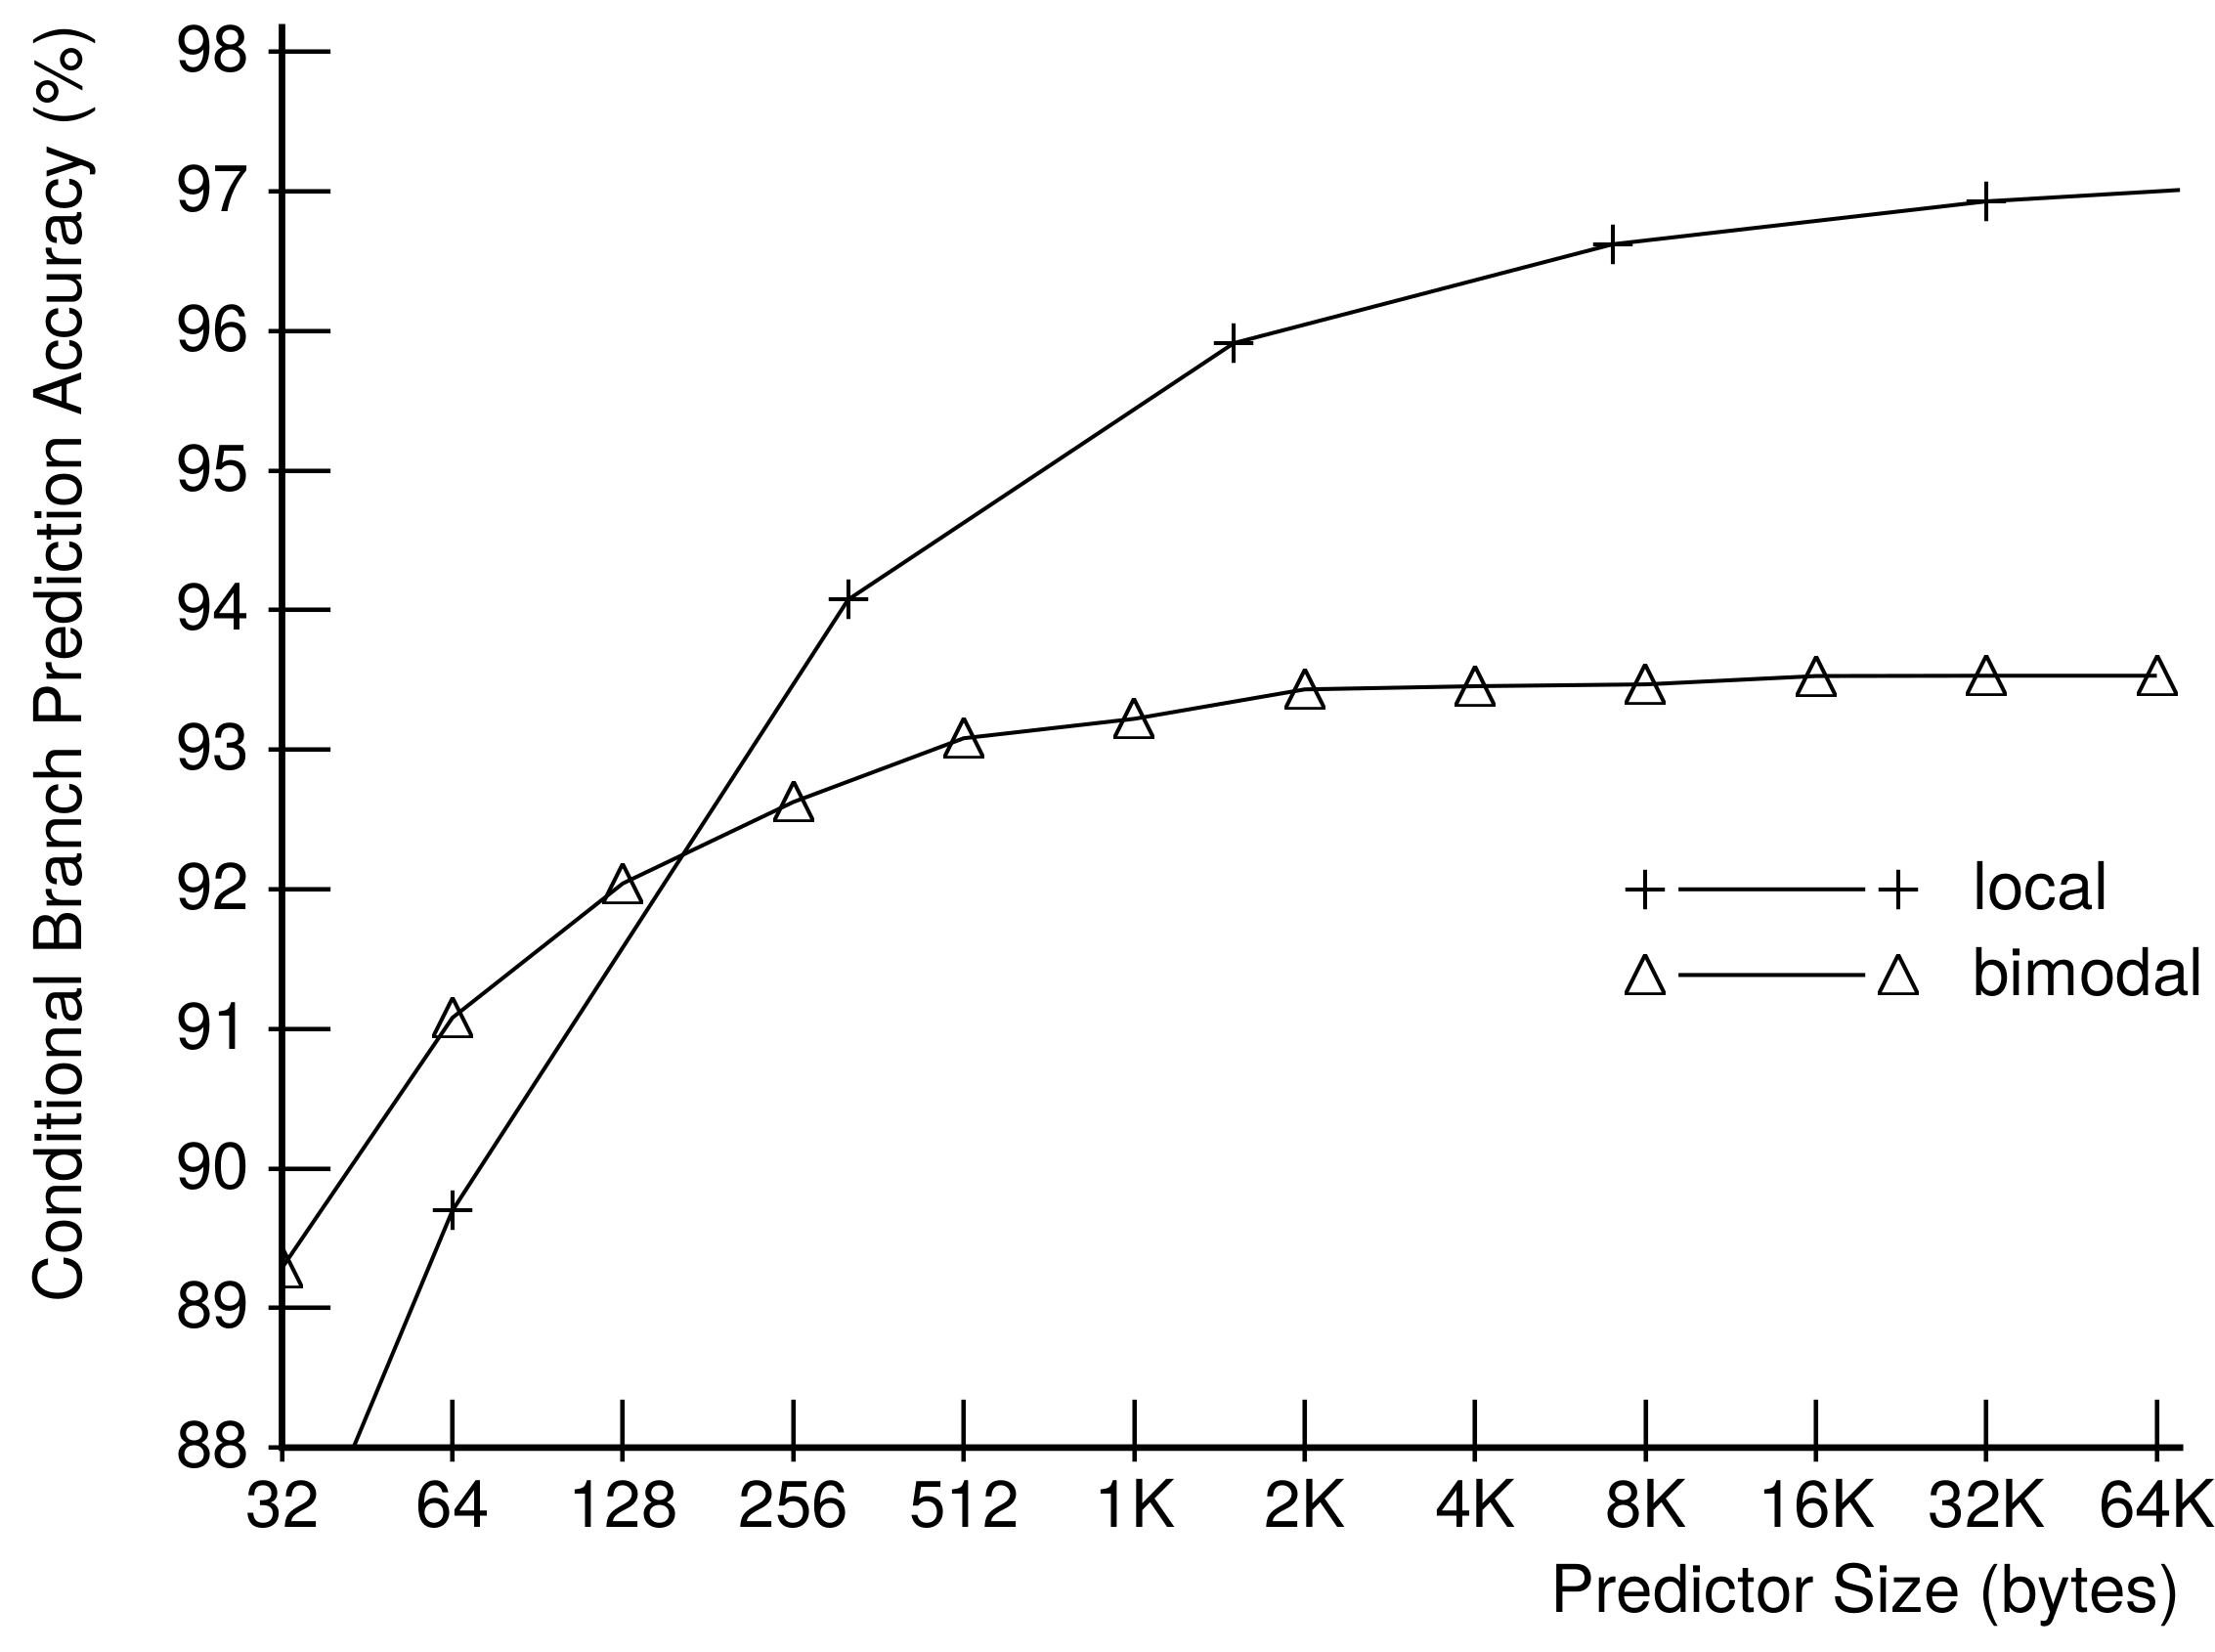
\includegraphics[height=0.8\textheight]{../bpred/mcf-local-bimodal}
\end{frame}

\begin{frame}{2-bit (bimodal) + local + global hist}
from McFarling, ``Combining Branch Predictors'' (1993)
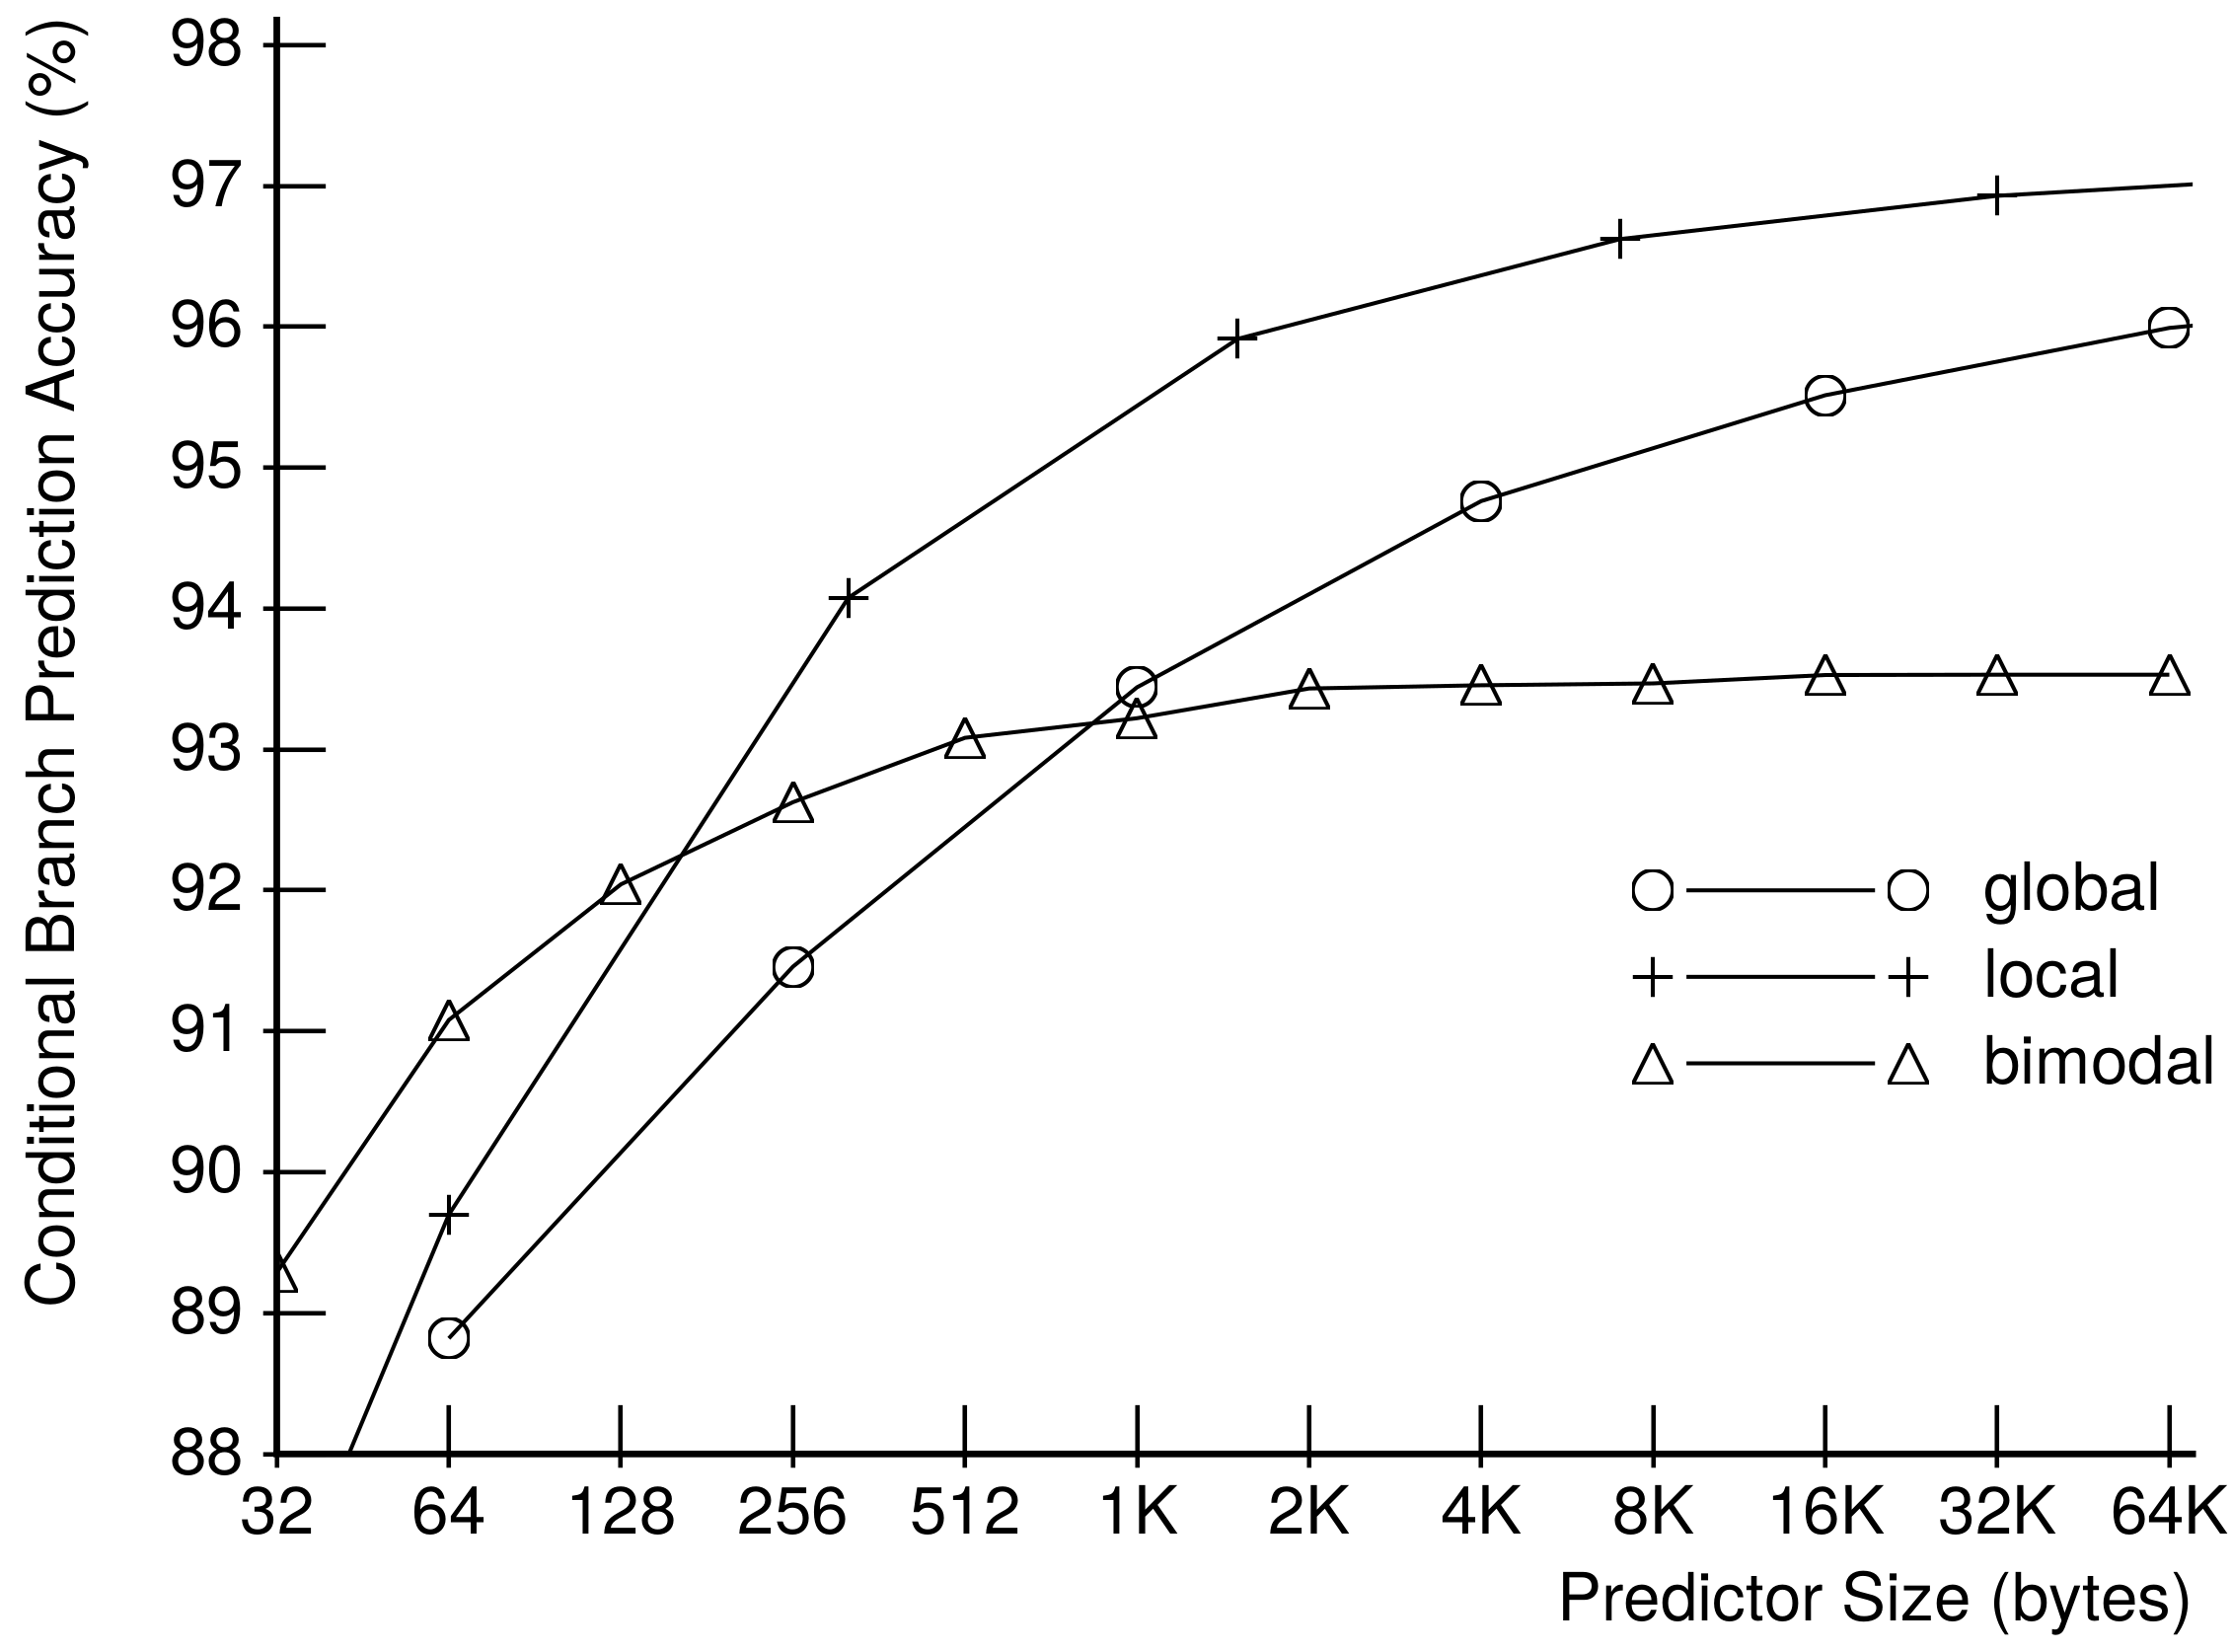
\includegraphics[height=0.8\textheight]{../bpred/mcf-local-bimodal-global}
\end{frame}

\begin{frame}{global + hash(global+PC) (gshare/gselect)}
from McFarling, ``Combining Branch Predictors'' (1993)
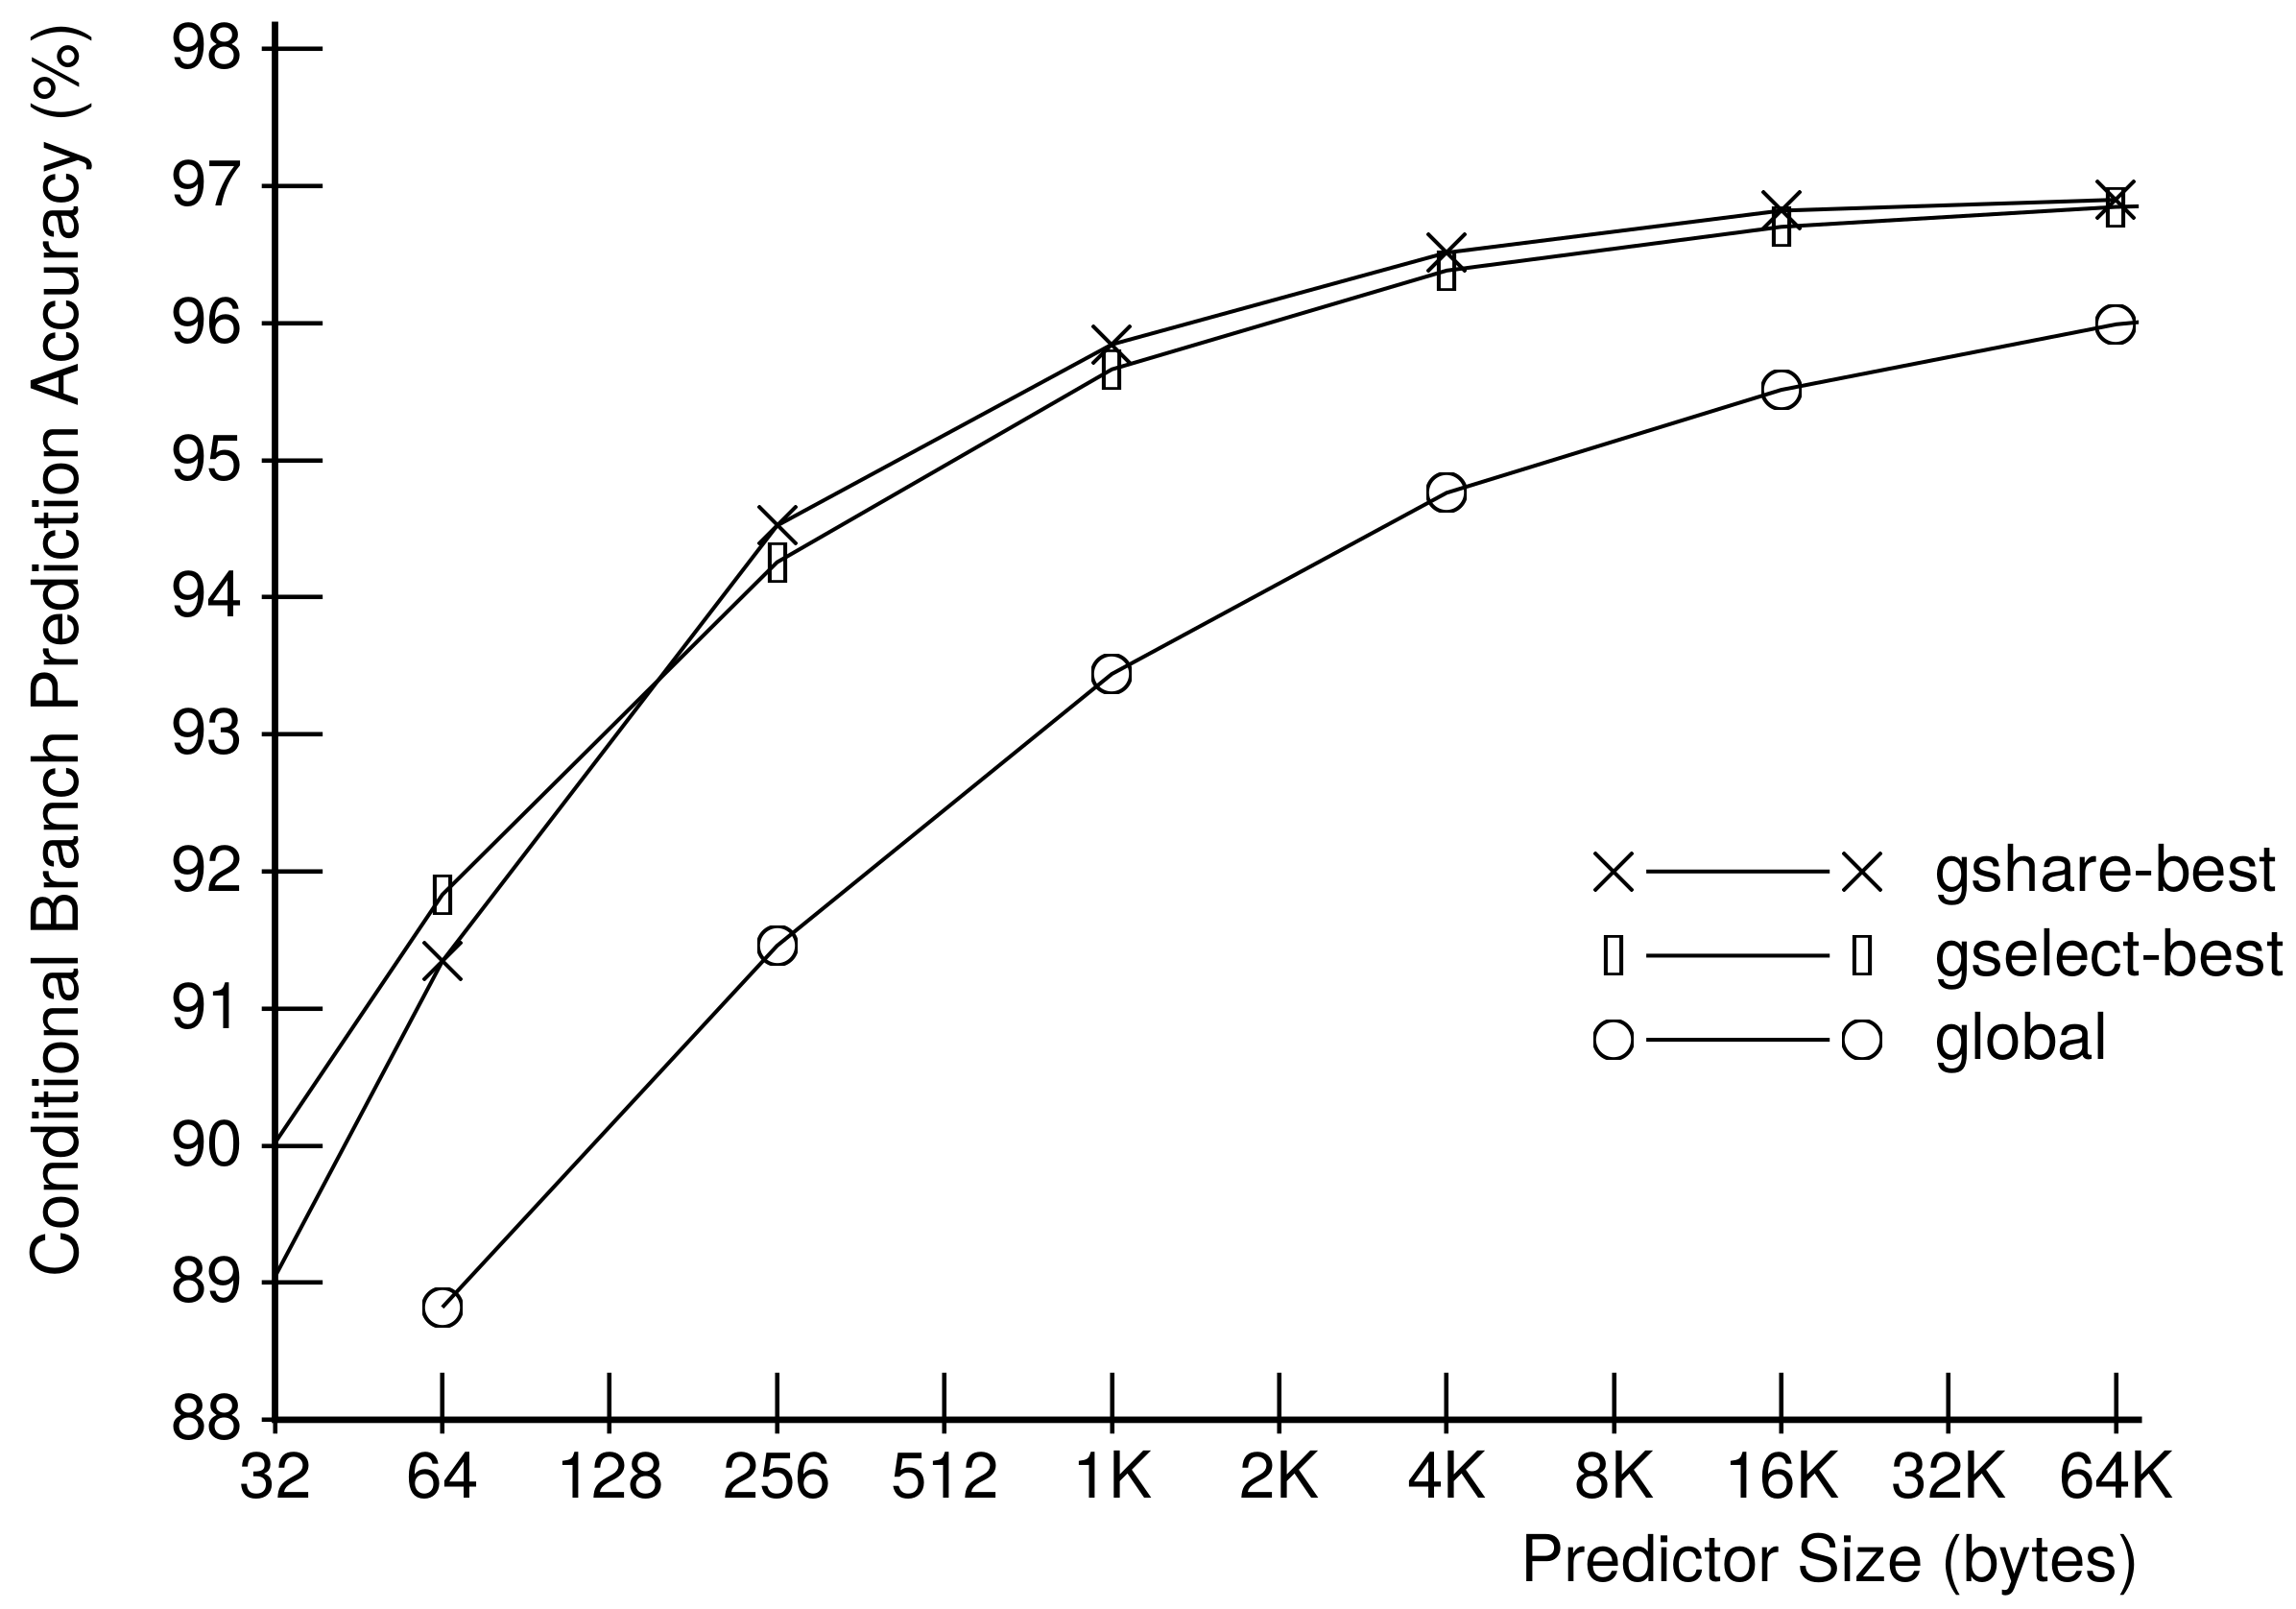
\includegraphics[height=0.8\textheight]{../bpred/mcf-global-gshare}
\end{frame}



\section{reversed engineering Haswell BP}
\begin{frame}{real BP?}
\begin{itemize}
\item details of modern CPU's branch predictors often not public
\item but\ldots
\vspace{.5cm}
\item Google Project Zero blog post with reverse engineered details
\item \scriptsize \url{https://googleprojectzero.blogspot.com/2018/01/reading-privileged-memory-with-side.html}
\item for RE'd BTB size:
\item \scriptsize \url{https://xania.org/201602/haswell-and-ivy-btb}
\end{itemize}
\end{frame}

\begin{frame}{reverse engineering Haswell BPs}
\begin{itemize}
\item branch target buffer
    \begin{itemize}
    \item 4-way, 4096 entries
    \item ignores bottom 4 bits of PC?
    \item hashes PC to index by shifting + XOR
    \item seems to store 32 bit offset from PC (not all 48+ bits of virtual addr)
    \end{itemize}
\item indirect branch predictor
    \begin{itemize}
    \item like the global history + PC predictor we showed, but\ldots
    \item uses history of recent branch addresses instead of taken/not taken
    \item keeps some info about last 29 branches
    \end{itemize}
\item what about conditional branches??? loops???
    \begin{itemize}
    \item couldn't find a reasonable source
    \end{itemize}
\end{itemize}
\end{frame}



\end{document}
